% Options for packages loaded elsewhere
\PassOptionsToPackage{unicode}{hyperref}
\PassOptionsToPackage{hyphens}{url}
%
\documentclass[
]{book}
\usepackage{amsmath,amssymb}
\usepackage{lmodern}
\usepackage{iftex}
\ifPDFTeX
  \usepackage[T1]{fontenc}
  \usepackage[utf8]{inputenc}
  \usepackage{textcomp} % provide euro and other symbols
\else % if luatex or xetex
  \usepackage{unicode-math}
  \defaultfontfeatures{Scale=MatchLowercase}
  \defaultfontfeatures[\rmfamily]{Ligatures=TeX,Scale=1}
\fi
% Use upquote if available, for straight quotes in verbatim environments
\IfFileExists{upquote.sty}{\usepackage{upquote}}{}
\IfFileExists{microtype.sty}{% use microtype if available
  \usepackage[]{microtype}
  \UseMicrotypeSet[protrusion]{basicmath} % disable protrusion for tt fonts
}{}
\makeatletter
\@ifundefined{KOMAClassName}{% if non-KOMA class
  \IfFileExists{parskip.sty}{%
    \usepackage{parskip}
  }{% else
    \setlength{\parindent}{0pt}
    \setlength{\parskip}{6pt plus 2pt minus 1pt}}
}{% if KOMA class
  \KOMAoptions{parskip=half}}
\makeatother
\usepackage{xcolor}
\usepackage{color}
\usepackage{fancyvrb}
\newcommand{\VerbBar}{|}
\newcommand{\VERB}{\Verb[commandchars=\\\{\}]}
\DefineVerbatimEnvironment{Highlighting}{Verbatim}{commandchars=\\\{\}}
% Add ',fontsize=\small' for more characters per line
\usepackage{framed}
\definecolor{shadecolor}{RGB}{248,248,248}
\newenvironment{Shaded}{\begin{snugshade}}{\end{snugshade}}
\newcommand{\AlertTok}[1]{\textcolor[rgb]{0.94,0.16,0.16}{#1}}
\newcommand{\AnnotationTok}[1]{\textcolor[rgb]{0.56,0.35,0.01}{\textbf{\textit{#1}}}}
\newcommand{\AttributeTok}[1]{\textcolor[rgb]{0.77,0.63,0.00}{#1}}
\newcommand{\BaseNTok}[1]{\textcolor[rgb]{0.00,0.00,0.81}{#1}}
\newcommand{\BuiltInTok}[1]{#1}
\newcommand{\CharTok}[1]{\textcolor[rgb]{0.31,0.60,0.02}{#1}}
\newcommand{\CommentTok}[1]{\textcolor[rgb]{0.56,0.35,0.01}{\textit{#1}}}
\newcommand{\CommentVarTok}[1]{\textcolor[rgb]{0.56,0.35,0.01}{\textbf{\textit{#1}}}}
\newcommand{\ConstantTok}[1]{\textcolor[rgb]{0.00,0.00,0.00}{#1}}
\newcommand{\ControlFlowTok}[1]{\textcolor[rgb]{0.13,0.29,0.53}{\textbf{#1}}}
\newcommand{\DataTypeTok}[1]{\textcolor[rgb]{0.13,0.29,0.53}{#1}}
\newcommand{\DecValTok}[1]{\textcolor[rgb]{0.00,0.00,0.81}{#1}}
\newcommand{\DocumentationTok}[1]{\textcolor[rgb]{0.56,0.35,0.01}{\textbf{\textit{#1}}}}
\newcommand{\ErrorTok}[1]{\textcolor[rgb]{0.64,0.00,0.00}{\textbf{#1}}}
\newcommand{\ExtensionTok}[1]{#1}
\newcommand{\FloatTok}[1]{\textcolor[rgb]{0.00,0.00,0.81}{#1}}
\newcommand{\FunctionTok}[1]{\textcolor[rgb]{0.00,0.00,0.00}{#1}}
\newcommand{\ImportTok}[1]{#1}
\newcommand{\InformationTok}[1]{\textcolor[rgb]{0.56,0.35,0.01}{\textbf{\textit{#1}}}}
\newcommand{\KeywordTok}[1]{\textcolor[rgb]{0.13,0.29,0.53}{\textbf{#1}}}
\newcommand{\NormalTok}[1]{#1}
\newcommand{\OperatorTok}[1]{\textcolor[rgb]{0.81,0.36,0.00}{\textbf{#1}}}
\newcommand{\OtherTok}[1]{\textcolor[rgb]{0.56,0.35,0.01}{#1}}
\newcommand{\PreprocessorTok}[1]{\textcolor[rgb]{0.56,0.35,0.01}{\textit{#1}}}
\newcommand{\RegionMarkerTok}[1]{#1}
\newcommand{\SpecialCharTok}[1]{\textcolor[rgb]{0.00,0.00,0.00}{#1}}
\newcommand{\SpecialStringTok}[1]{\textcolor[rgb]{0.31,0.60,0.02}{#1}}
\newcommand{\StringTok}[1]{\textcolor[rgb]{0.31,0.60,0.02}{#1}}
\newcommand{\VariableTok}[1]{\textcolor[rgb]{0.00,0.00,0.00}{#1}}
\newcommand{\VerbatimStringTok}[1]{\textcolor[rgb]{0.31,0.60,0.02}{#1}}
\newcommand{\WarningTok}[1]{\textcolor[rgb]{0.56,0.35,0.01}{\textbf{\textit{#1}}}}
\usepackage{longtable,booktabs,array}
\usepackage{calc} % for calculating minipage widths
% Correct order of tables after \paragraph or \subparagraph
\usepackage{etoolbox}
\makeatletter
\patchcmd\longtable{\par}{\if@noskipsec\mbox{}\fi\par}{}{}
\makeatother
% Allow footnotes in longtable head/foot
\IfFileExists{footnotehyper.sty}{\usepackage{footnotehyper}}{\usepackage{footnote}}
\makesavenoteenv{longtable}
\usepackage{graphicx}
\makeatletter
\def\maxwidth{\ifdim\Gin@nat@width>\linewidth\linewidth\else\Gin@nat@width\fi}
\def\maxheight{\ifdim\Gin@nat@height>\textheight\textheight\else\Gin@nat@height\fi}
\makeatother
% Scale images if necessary, so that they will not overflow the page
% margins by default, and it is still possible to overwrite the defaults
% using explicit options in \includegraphics[width, height, ...]{}
\setkeys{Gin}{width=\maxwidth,height=\maxheight,keepaspectratio}
% Set default figure placement to htbp
\makeatletter
\def\fps@figure{htbp}
\makeatother
\setlength{\emergencystretch}{3em} % prevent overfull lines
\providecommand{\tightlist}{%
  \setlength{\itemsep}{0pt}\setlength{\parskip}{0pt}}
\setcounter{secnumdepth}{5}
\usepackage{booktabs}
\usepackage{amsthm}
\makeatletter
\def\thm@space@setup{%
  \thm@preskip=8pt plus 2pt minus 4pt
  \thm@postskip=\thm@preskip
}
\makeatother
\ifLuaTeX
  \usepackage{selnolig}  % disable illegal ligatures
\fi
\usepackage[]{natbib}
\bibliographystyle{apalike}
\IfFileExists{bookmark.sty}{\usepackage{bookmark}}{\usepackage{hyperref}}
\IfFileExists{xurl.sty}{\usepackage{xurl}}{} % add URL line breaks if available
\urlstyle{same} % disable monospaced font for URLs
\hypersetup{
  pdftitle={Visualising Data using R},
  pdfauthor={Craig Alexander, Eilidh Jack \& Marnie Low},
  hidelinks,
  pdfcreator={LaTeX via pandoc}}

\title{Visualising Data using R}
\author{Craig Alexander, Eilidh Jack \& Marnie Low}
\date{}

\begin{document}
\maketitle

{
\setcounter{tocdepth}{1}
\tableofcontents
}
\hypertarget{overview}{%
\chapter{Overview}\label{overview}}

The R programming language provides researchers with access to a large range of fully customisable data visualisation options, which are typically not available in point-and-click software. These visualisations are not only visually appealing, but can increase transparency about the distribution of the underlying data, rather than relying on commonly used visualisations of aggregations.

In this introductory section of our course, we will provide a practical introduction to using R, particularly in how to visualise data which you will use throughout the course. First, we will explain the rationale behind using R for data visualisation using the \texttt{ggplot2} package. This package will allow us to begin with common plotting outputs such as histograms and boxplots, and extend to more complex structures used within spatial data visualisation.

\hypertarget{the-ggplot2-package}{%
\section{\texorpdfstring{The \texttt{ggplot2} package}{The ggplot2 package}}\label{the-ggplot2-package}}

There are a host of options to data visualisation in R. In this course, we will mainly use the \texttt{ggplot2} package, which forms part of the larger \texttt{tidyverse} collection of packages which provide functions for efficient data management in R. We will also use eother packages within \texttt{tidyverse} in the course.

A grammar of graphics is a standardised way to describe the components of a graphic. \texttt{ggplot2} uses a layered grammar of graphics, in which plots are bulit up in a series of layers. It may be helpful to think about any picture as having multiple elements that sit semi-transparently over each other.
Figure \ref{fig:layerplot} shows the evolution of a sumple scatterplot using this layered approach. First, the plot space is built (layer 1); the variables are specified (layer 2); the type of visualisation that is desired for these variables is specified (layer 3) - in this case \texttt{geom\_point()}is called to visualise individual data points; a second \texttt{geom} layer is added to include a line of best fit (layer 4); the axis labels are editied for readability (layer 5) and finally, a theme is applied to change the overall appearance of the plot (layer 6).

\begin{figure}[h]

{\centering 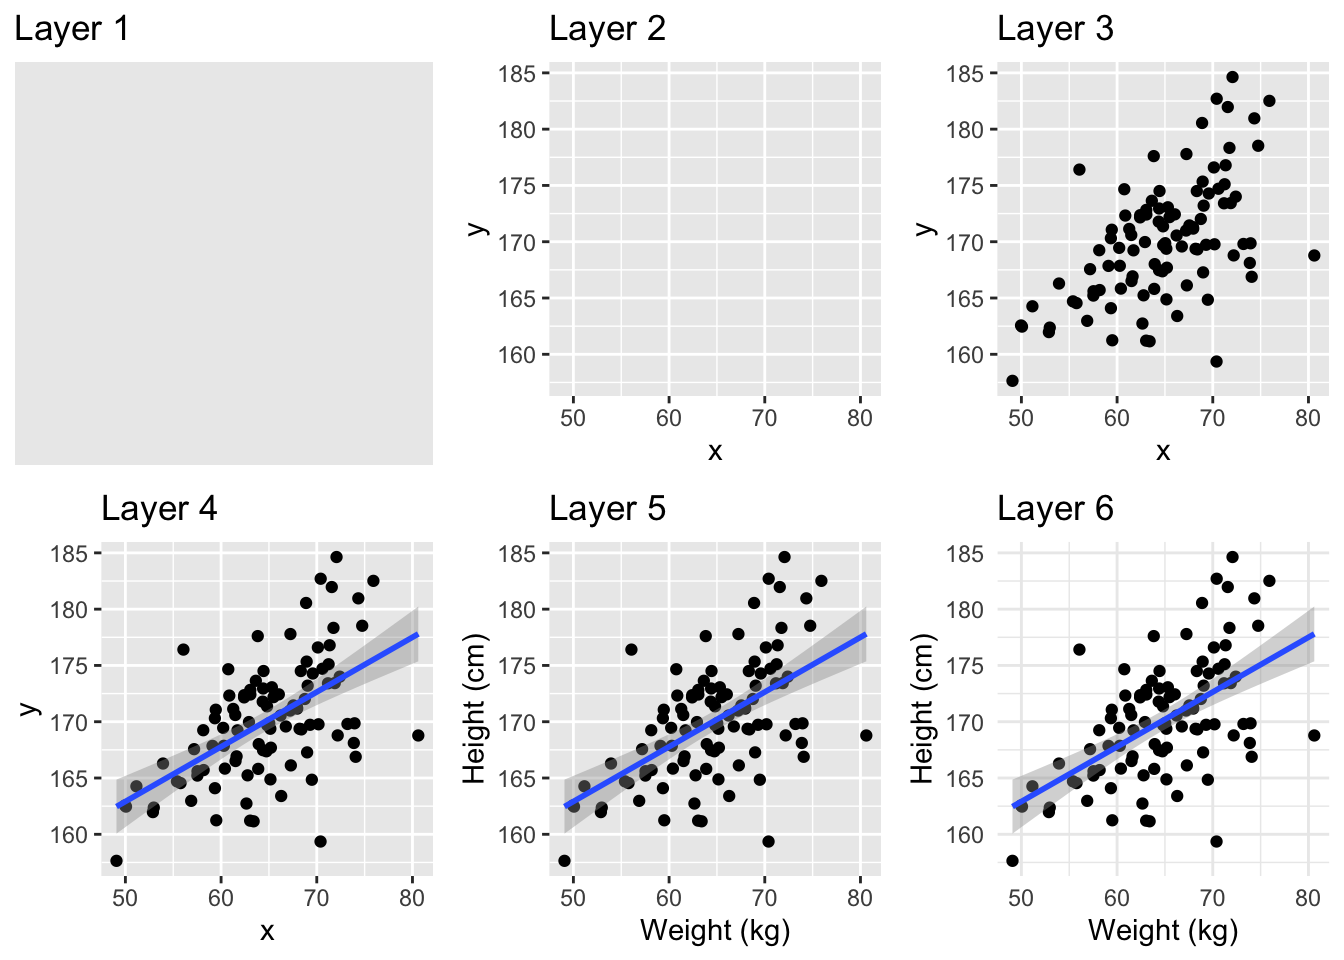
\includegraphics[width=0.8\linewidth]{bookdown-demo_files/figure-latex/layerplot-1} 

}

\caption{\label{fig:layer} Evolution of a layered plot.}\label{fig:layerplot}
\end{figure}

Each layer is independent and individually customisable. For example, the size, colour and position of each component can be adjusted. The use of layers makes it easy to build up complex plots step-by-step, and to adapt or extend plots from existing code.

\hypertarget{data}{%
\section{Data}\label{data}}

In this course, we will use some datasets for analysis. You can download these from the following repository:

\href{https://github.com/craigalexander/IntroToRDataVis/tree/main/Data}{Link to repository}

\hypertarget{libraries}{%
\section{Libraries}\label{libraries}}

Throughout this week, we will use some libraries within R for modelling and data visualisation. You will need the following libraries installed on your version of R:

\begin{itemize}
\tightlist
\item
  \texttt{tidyverse}
\item
  \texttt{lubridate}
\item
  \texttt{magrittr}
\item
  \texttt{MASS}
\item
  \texttt{ggmap}
\item
  \texttt{plotly}
\item
  \texttt{mgcv}
\item
  \texttt{sp}
\item
  \texttt{splines}
\item
  \texttt{gratia}
\item
  \texttt{spdep}
\item
  \texttt{sf}
\item
  \texttt{CARBayes}
\item
  \texttt{CARBayesST}
\item
  \texttt{RColorBrewer}
\item
  \texttt{gridExtra}
\item
  \texttt{leaflet}
\end{itemize}

\hypertarget{intro}{%
\chapter{Getting Started}\label{intro}}

\hypertarget{setting-up-r}{%
\section{Setting up R}\label{setting-up-r}}

You need to have access to \href{https://www.r-project.org/}{R} for this course. You can download R for free from \href{https://cran.r-project.org/}{CRAN}.

R is available for Windows, Mac OS and Linux as well as some less common platforms.

You can download the standard version of R from \href{https://cran.r-project.org/}{CRAN}.

\hypertarget{downloading-and-installing-r-for-windows}{%
\subsection{Downloading and installing R for Windows}\label{downloading-and-installing-r-for-windows}}

To download the Windows installer of R, just enter the following URL (or click on the clink).

\url{https://cran.r-project.org//bin/windows/base/release.html}

This will download the most installer for the most recent version of R. Alternatively, you can go to the main CRAN page, \url{https://cran.r-project.org/}, and then click on ``Download R for Windows'', click on ``base'' and then on ``Download R x.y.z for Windows'' (where x.y.z is the current version number of R).

You can then run the installer, accepting all default settings.

\hypertarget{downloading-and-installing-r-for-mac}{%
\subsection{Downloading and installing R for Mac}\label{downloading-and-installing-r-for-mac}}

To download the Windows installer for Mac, just enter the following URL (or click on the clink).

\url{https://cran.r-project.org/bin/macosx/}

From here, select the most recent version of R and the .pkg file will automatically download. This file will be in the form ``R-x.y.z'' (where x.y.z is the current version number of R).

Once the file is opened, the installer will open and you can select the default settings.

\hypertarget{rstudio}{%
\section{RStudio}\label{rstudio}}

It is recommended that you also download and install \href{https://www.rstudio.com/products/rstudio/download/}{RStudio Desktop}, a powerful \href{https://en.wikipedia.org/wiki/Integrated_development_environment}{integrated development environment (IDE)} for R. RStudio contains a much better code editor. It has, for example, \href{https://en.wikipedia.org/wiki/Syntax_highlighting}{syntax highlighting}, i.e.~it will automatically display your code in different colours to make it easier and quicker to read the code. Even though other IDEs, such as \href{http://www.walware.de/goto/statet}{Eclipse}, \href{https://code.visualstudio.com/}{Visual Studio Code}, or \href{https://ess.r-project.org/}{Emacs} can also be used with R, RStudio is by far the most popular among R users.

RStudio is just a front-end for R, so to be able make use of RStudio, you need to also have R installed.

RStudio Desktop Open Source is available for free from \href{https://rstudio.com}{RStudio}.

\hypertarget{installing-rstudio-for-windowsmac}{%
\subsection{Installing RStudio for Windows/Mac}\label{installing-rstudio-for-windowsmac}}

Go to

\url{https://www.rstudio.com/products/rstudio/download/}

and scroll down to the section ``All installers'', then click on ``RStudio-x-y-z.exe'' in the first row of the table for a Windows install, or click on ``RStudio-x-y-z.dmg'' for a macOS install. This should start the download of the RStudio installer.

You can then run the installer, accepting all default settings (for macOS, you will need to drag and drop the application into the applications folder once open).

\hypertarget{r-packages}{%
\section{R packages}\label{r-packages}}

R comes with a default selection of packages, which should cover your ``basic needs'' in terms of data management, data visualisation and modelling. However, there is a large selection of ``add-on'' R packages available on CRAN, some of which we will use in this course. You can only use these R packages once you have installed them.

Imagine you want to use an R package called \texttt{ggplot2} (which we will use later in this course). In order to be able to use it, you first need to install it. You can do so by entering

\begin{Shaded}
\begin{Highlighting}[]
\FunctionTok{install.packages}\NormalTok{(}\StringTok{"ggplot2"}\NormalTok{)}
\end{Highlighting}
\end{Shaded}

into R. This will download and install the package \texttt{ggplot2}, as well as any other packages \texttt{ggplot} uses.

Alternatively, you can click on the tab ``Packages in the bottom-right panel, and then click on''Install''.

\begin{figure}

{\centering 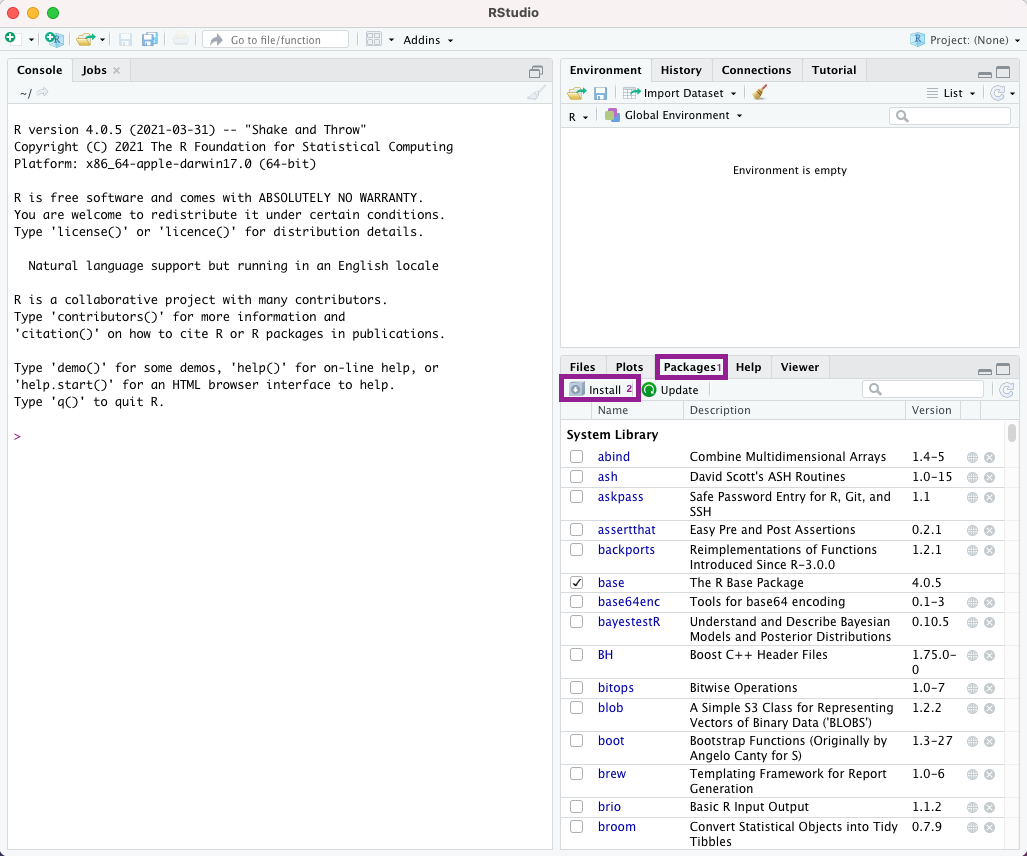
\includegraphics[width=0.85\linewidth]{Packages_Install} 

}

\caption{Selecting the installation menu for installing packages}\label{fig:install1}
\end{figure}

You can then enter the name of the package you want to install and click on ``Install''

\begin{figure}

{\centering 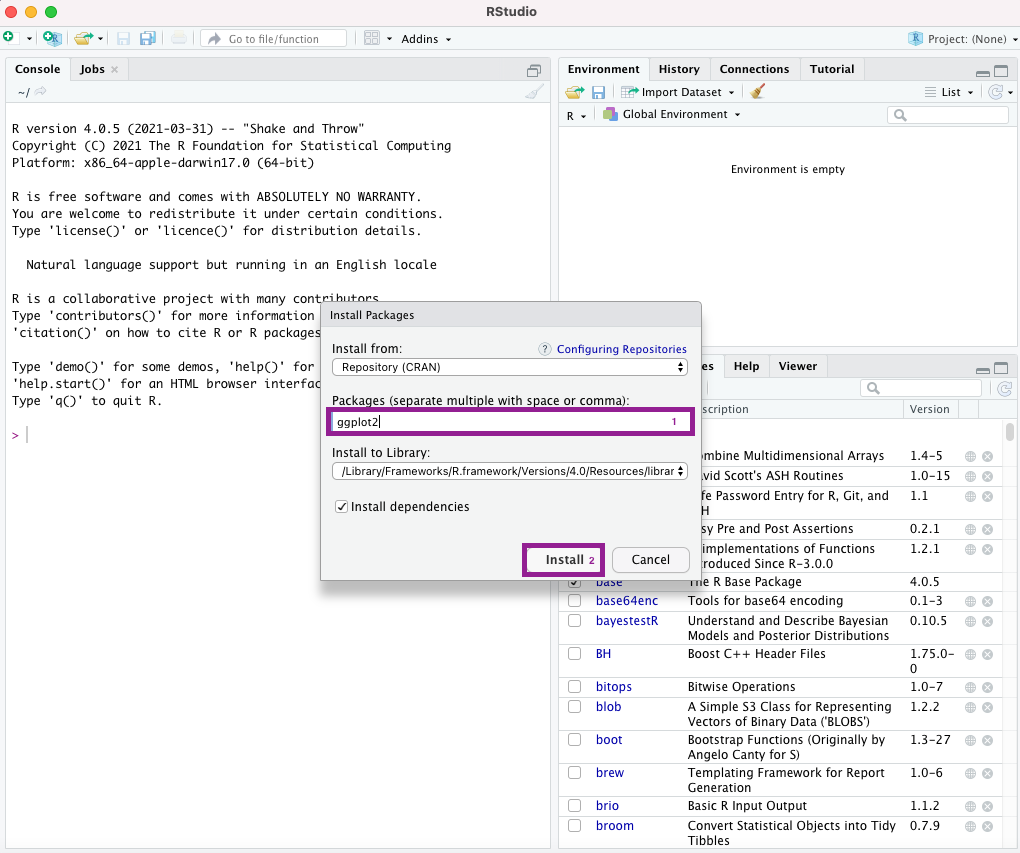
\includegraphics[width=0.85\linewidth]{Packages_Installed} 

}

\caption{Installation menu for packages}\label{fig:install2}
\end{figure}

Once you have installed an R package, you can load it using the function \texttt{library}

\begin{Shaded}
\begin{Highlighting}[]
\FunctionTok{library}\NormalTok{(ggplot2)}
\end{Highlighting}
\end{Shaded}

\hypertarget{efficient-data-management-in-r}{%
\chapter{Efficient Data Management in R}\label{efficient-data-management-in-r}}

\hypertarget{tidyverse}{%
\section{Tidyverse}\label{tidyverse}}

\href{https://www.tidyverse.org/}{Tidyverse} is a collection of R packages designed to help data scientists to make more efficient use of R. It contains the following packages (and several more, which we will:

\begin{itemize}
\tightlist
\item
  \href{http://tibble.tidyverse.org/}{tibble} provides a ``modern reimagining'' of the standard \texttt{data.frame}, in R. Tibbles (or \texttt{tbl\_df}s) are more flexible in terms of what they can store, but (purposefully) less flexible in terms of ``sloppy code''.
\item
  \href{http://readr.tidyverse.org/}{readr} provides alternative functions for reading in text data in tabular form. It provides faster and more consistent alternatives to \texttt{read.table} and \texttt{read.csv}.
\item
  \href{http://dplyr.tidyverse.org/}{dplyr} provides a powerful suite of functions for data manipulation with a focus on allowing for clean and simple code. We will look at \texttt{dplyr} in more detail this week.
\item
  \href{http://ggplot2.tidyverse.org/}{ggplot2} is a very featureful and systematic set of plotting functions, which we will focus on in this tutorial.
\item
  \href{https://lubridate.tidyverse.org/}{lubridate} is a very useful package for handling dates and times in R. Dates and times are often tricky to deal with, and \texttt{lubridate} provides many useful functions for efficiently handling these.
\end{itemize}

\hypertarget{pipelines}{%
\section{Pipelines}\label{pipelines}}

Pipelines are at the centre of all the tidyverse packages. The R package \href{https://cran.r-project.org/web/packages/magrittr/}{magrittr} provides a forward-pipe operator for R.

Suppose we have a function \texttt{f} defined in R

\begin{Shaded}
\begin{Highlighting}[]
\NormalTok{f }\OtherTok{\textless{}{-}} \ControlFlowTok{function}\NormalTok{(x)}
\NormalTok{  x}\SpecialCharTok{\^{}}\DecValTok{2}
\end{Highlighting}
\end{Shaded}

Then we can apply \texttt{f} to an argument \texttt{x} using

\begin{Shaded}
\begin{Highlighting}[]
\NormalTok{x }\OtherTok{\textless{}{-}} \DecValTok{3}
\FunctionTok{f}\NormalTok{(x)}
\end{Highlighting}
\end{Shaded}

\begin{verbatim}
## [1] 9
\end{verbatim}

The forward-pipes from magrittr allow us to rewrite this function call as

\begin{Shaded}
\begin{Highlighting}[]
\NormalTok{x }\SpecialCharTok{\%\textgreater{}\%}\NormalTok{ f}
\end{Highlighting}
\end{Shaded}

\begin{verbatim}
## [1] 9
\end{verbatim}

instead. The advantage of this alternative notation might not become immediately clear, but its advantage becomes more obvious when looking at nested function calls.

Consider the R data set \texttt{mtcars}, which contains data from the 1974 edition from the US magazine Motor Trend. Suppose we want to convert the fuel consumption to litres per 100 kilometres and then only retain the cars with a fuel economy better than 10 litres per 100 kilometres.

\begin{Shaded}
\begin{Highlighting}[]
\NormalTok{mtcars2 }\OtherTok{\textless{}{-}} \FunctionTok{transform}\NormalTok{(mtcars, }\AttributeTok{lp100k=}\FloatTok{235.21}\SpecialCharTok{/}\NormalTok{mpg)}
\FunctionTok{subset}\NormalTok{(mtcars2, lp100k}\SpecialCharTok{\textless{}=}\DecValTok{10}\NormalTok{)}
\end{Highlighting}
\end{Shaded}

\begin{verbatim}
##                 mpg cyl  disp  hp drat    wt  qsec vs am gear carb   lp100k
## Merc 240D      24.4   4 146.7  62 3.69 3.190 20.00  1  0    4    2 9.639754
## Fiat 128       32.4   4  78.7  66 4.08 2.200 19.47  1  1    4    1 7.259568
## Honda Civic    30.4   4  75.7  52 4.93 1.615 18.52  1  1    4    2 7.737171
## Toyota Corolla 33.9   4  71.1  65 4.22 1.835 19.90  1  1    4    1 6.938348
## Fiat X1-9      27.3   4  79.0  66 4.08 1.935 18.90  1  1    4    1 8.615751
## Porsche 914-2  26.0   4 120.3  91 4.43 2.140 16.70  0  1    5    2 9.046538
## Lotus Europa   30.4   4  95.1 113 3.77 1.513 16.90  1  1    5    2 7.737171
\end{verbatim}

(If you are wondering where the number of 235.21 comes from: A US gallon is roughly 3.785 litres and a mile is roughly 1.609 kilometres, and \(\frac{100\times 3.785}{1.609}\approx 235.21\))

If we want to perform both steps in one go, we can nest the two calls within one another and use

\begin{Shaded}
\begin{Highlighting}[]
\FunctionTok{subset}\NormalTok{(}\FunctionTok{transform}\NormalTok{(mtcars, }\AttributeTok{lp100k=}\FloatTok{235.21}\SpecialCharTok{/}\NormalTok{mpg), lp100k}\SpecialCharTok{\textless{}=}\DecValTok{10}\NormalTok{)}
\end{Highlighting}
\end{Shaded}

This gives exactly the same results, but is not very easy to read and understand. It is not easy to see that the argument \texttt{lp100k\textless{}=10} belongs to \texttt{subset}. When nesting function calls, the arguments get increasingly far from the function call to which they belong.

The \texttt{\%\textgreater{}\%} operator however allows us to write this much more cleanly:

\begin{Shaded}
\begin{Highlighting}[]
\NormalTok{mtcars }\SpecialCharTok{\%\textgreater{}\%}
  \FunctionTok{transform}\NormalTok{(}\AttributeTok{lp100k=}\FloatTok{235.21}\SpecialCharTok{/}\NormalTok{mpg) }\SpecialCharTok{\%\textgreater{}\%}
  \FunctionTok{subset}\NormalTok{(lp100k}\SpecialCharTok{\textless{}=}\DecValTok{10}\NormalTok{)}
\end{Highlighting}
\end{Shaded}

\hypertarget{task}{%
\subsection{Task}\label{task}}

The R code below uses pipelines. Convert it to nested function calls.

\begin{Shaded}
\begin{Highlighting}[]
\FunctionTok{rnorm}\NormalTok{(}\DecValTok{1000}\NormalTok{) }\SpecialCharTok{\%\textgreater{}\%} \FunctionTok{sin}\NormalTok{() }\SpecialCharTok{\%\textgreater{}\%} \FunctionTok{max}\NormalTok{()}
\end{Highlighting}
\end{Shaded}

\hypertarget{solution}{%
\subsection{Solution}\label{solution}}

The code generates a random sample of size 1000 (from a standard normal distribution), computes the sine of each entry and then takes the maximum.

\begin{Shaded}
\begin{Highlighting}[]
\FunctionTok{max}\NormalTok{(}\FunctionTok{sin}\NormalTok{(}\FunctionTok{rnorm}\NormalTok{(}\DecValTok{1000}\NormalTok{)))}
\end{Highlighting}
\end{Shaded}

\begin{verbatim}
## [1] 0.9999919
\end{verbatim}

In this case the nested function call is easy to read because every function only takes one argument.

\hypertarget{task-1}{%
\subsection{Task}\label{task-1}}

Convert the R code below to pipelines.

\begin{Shaded}
\begin{Highlighting}[]
\FunctionTok{library}\NormalTok{(MASS)                       }\CommentTok{\# Load package MASS, which contains the data}
\FunctionTok{subset}\NormalTok{(}\FunctionTok{transform}\NormalTok{(mammals, }\AttributeTok{ratio=}\NormalTok{brain}\SpecialCharTok{/}\NormalTok{body), ratio}\SpecialCharTok{==}\FunctionTok{max}\NormalTok{(ratio))}
\end{Highlighting}
\end{Shaded}

\hypertarget{answer}{%
\subsection{Answer}\label{answer}}

You can use the following R code using pipelines.

\begin{Shaded}
\begin{Highlighting}[]
\FunctionTok{library}\NormalTok{(MASS)}
\NormalTok{mammals }\SpecialCharTok{\%\textgreater{}\%}
  \FunctionTok{transform}\NormalTok{(}\AttributeTok{ratio=}\NormalTok{brain}\SpecialCharTok{/}\NormalTok{body) }\SpecialCharTok{\%\textgreater{}\%}
  \FunctionTok{subset}\NormalTok{(ratio}\SpecialCharTok{==}\FunctionTok{max}\NormalTok{(ratio))}
\end{Highlighting}
\end{Shaded}

\begin{verbatim}
##                  body brain    ratio
## Ground squirrel 0.101     4 39.60396
\end{verbatim}

Oddly enough, ground squirrels have a higher brain-to-body weight ratio than humans.

\hypertarget{additional-resources}{%
\subsection{Additional Resources}\label{additional-resources}}

\href{\%22https://speakerdeck.com/hadley/pipelines-for-data-analysis-in-r\%22}{Pipelines for Data Analysis in R}
Hadley Wickham has produced a series of excellent slides about pipelines, which covers much of what we will look at in this tutorial.

\href{\%22http://r4ds.had.co.nz/pipes.html\%22}{Background reading: Chapter 18 of R for Data Science}
Chapter 18 of \emph{R for Data Science} gives a detailed overview of pipes and some of the underpinning technology (though the latter is rather advanced).

\hypertarget{tibbles}{%
\section{Tibbles}\label{tibbles}}

The package \href{https://cran.r-project.org/web/packages/tibble/}{tibble} provides \texttt{tbl\_df}'s (or ``tibbles'', which is easier to pronounce). They are a modern take on the built-in class \texttt{data.frame}.

One key advantage of tibbles is that they can store anything. A \texttt{data.frame} can only store a single value per ``cell'', for example a number or a character string. However, in a tibble, you can store a list or even another tibble in a cell. An example of this is the tibble \texttt{starwars} from the package \texttt{dplyr}. The column \texttt{starships} contains for each row the list of starships flown by that character (which is a list of different length depending on the character.)

\begin{Shaded}
\begin{Highlighting}[]
\FunctionTok{library}\NormalTok{(dplyr)                             }\CommentTok{\# Load library dplyr which contains the data}
\NormalTok{starwars[,}\FunctionTok{c}\NormalTok{(}\StringTok{"name"}\NormalTok{, }\StringTok{"starships"}\NormalTok{)]          }\CommentTok{\# Print columns name and starships}
\end{Highlighting}
\end{Shaded}

\begin{verbatim}
## # A tibble: 87 x 2
##    name               starships
##    <chr>              <list>   
##  1 Luke Skywalker     <chr [2]>
##  2 C-3PO              <chr [0]>
##  3 R2-D2              <chr [0]>
##  4 Darth Vader        <chr [1]>
##  5 Leia Organa        <chr [0]>
##  6 Owen Lars          <chr [0]>
##  7 Beru Whitesun lars <chr [0]>
##  8 R5-D4              <chr [0]>
##  9 Biggs Darklighter  <chr [1]>
## 10 Obi-Wan Kenobi     <chr [5]>
## # ... with 77 more rows
\end{verbatim}

\begin{Shaded}
\begin{Highlighting}[]
\NormalTok{starwars[}\DecValTok{10}\NormalTok{,}\StringTok{"starships"}\NormalTok{][[}\DecValTok{1}\NormalTok{]]              }\CommentTok{\# Starships flown by Obi{-}Wan}
\end{Highlighting}
\end{Shaded}

\begin{verbatim}
## [[1]]
## [1] "Jedi starfighter"         "Trade Federation cruiser"
## [3] "Naboo star skiff"         "Jedi Interceptor"        
## [5] "Belbullab-22 starfighter"
\end{verbatim}

We could not have stored this information in a data frame. We would have had to either store the information across several data frames or stored the list of starships as a character string.

\hypertarget{creating-tibbles}{%
\subsection{Creating tibbles}\label{creating-tibbles}}

We can create tibbles using the function \texttt{tibble}. We can create the tibble from above using

\begin{Shaded}
\begin{Highlighting}[]
\NormalTok{kidstibble }\OtherTok{\textless{}{-}} \FunctionTok{tibble}\NormalTok{(}\AttributeTok{name=}\FunctionTok{c}\NormalTok{(}\StringTok{"Sarah"}\NormalTok{, }\StringTok{"John"}\NormalTok{), }\AttributeTok{age=}\FunctionTok{c}\NormalTok{(}\DecValTok{4}\NormalTok{,}\DecValTok{11}\NormalTok{), }\AttributeTok{weight=}\FunctionTok{c}\NormalTok{(}\DecValTok{15}\NormalTok{,}\DecValTok{28}\NormalTok{),}
                     \AttributeTok{height=}\FunctionTok{c}\NormalTok{(}\DecValTok{101}\NormalTok{,}\DecValTok{132}\NormalTok{), }\AttributeTok{gender=}\FunctionTok{c}\NormalTok{(}\StringTok{"f"}\NormalTok{, }\StringTok{"m"}\NormalTok{))}
\end{Highlighting}
\end{Shaded}

In other words, the function \texttt{tibble} assembles a tibble on a column-by-column basis (akin to using \texttt{cbind}).

The function \texttt{tribble} (``transposed tibble'') lets you create a tibble on a row-by-bow basis (akin to using \texttt{rbind}), which is typically more legible when creating a matrix in code.

\begin{Shaded}
\begin{Highlighting}[]
\NormalTok{kidstibble }\OtherTok{\textless{}{-}} \FunctionTok{tribble}\NormalTok{(}\SpecialCharTok{\textasciitilde{}}\NormalTok{name,   }\SpecialCharTok{\textasciitilde{}}\NormalTok{age, }\SpecialCharTok{\textasciitilde{}}\NormalTok{weight, }\SpecialCharTok{\textasciitilde{}}\NormalTok{height, }\SpecialCharTok{\textasciitilde{}}\NormalTok{gender,}
                      \StringTok{"Sarah"}\NormalTok{,    }\DecValTok{4}\NormalTok{,      }\DecValTok{15}\NormalTok{,     }\DecValTok{101}\NormalTok{,     }\StringTok{"f"}\NormalTok{,}
                      \StringTok{"John"}\NormalTok{,    }\DecValTok{11}\NormalTok{,      }\DecValTok{28}\NormalTok{,     }\DecValTok{132}\NormalTok{,     }\StringTok{"m"}\NormalTok{)}
\end{Highlighting}
\end{Shaded}

\hypertarget{working-with-tibbles}{%
\subsection{Working with tibbles}\label{working-with-tibbles}}

\begin{itemize}
\tightlist
\item
  Variables/Columns can be accessed and added using \texttt{tibble\$varname} (\texttt{varname} needs to be fully spelled out). You can also access a column using \texttt{tibble{[},"varname"{]}} or \texttt{tibble{[}{[}"varname"{]}{]}}.
\item
  Rows can be selected using \texttt{tibble{[}rowindices,{]}} (note that you cannot use row names).
\item
  Individual cells can be accessed using \texttt{tibble{[}rowindices,\ colindices{]}}.
\end{itemize}

\hypertarget{subsetting-tibbles-always-results-in-a-tibble}{%
\subsection{Subsetting tibbles always results in a tibble}\label{subsetting-tibbles-always-results-in-a-tibble}}

Tibbles are also more consistent. Subsetting tibbles always results in a tibble.

\begin{Shaded}
\begin{Highlighting}[]
\NormalTok{kidstibble[,}\DecValTok{1}\NormalTok{]                            }\CommentTok{\# Result is a tibble}
\end{Highlighting}
\end{Shaded}

\begin{verbatim}
## # A tibble: 2 x 1
##   name 
##   <chr>
## 1 Sarah
## 2 John
\end{verbatim}

In contrast, subsetting a data frame or matrix is not guaranteed to result in a data frame or matrix (unless you use \texttt{drop=FALSE}). If the result is a single column or row, subsetting a data frame or matrix results in a vector.

This ``dropping'' of the dimension can be very useful when using R interactively, but can be the source of many issues in more complex projects, when programmers incorrectly assume that subsetting a data frame or matrix will always result in another data frame or matrix, rather than possibly just a vector (it is thus a good idea to always use \texttt{drop=FALSE} when working with data frames or matrices in complex projects).

\href{\%22https://github.com/rstudio/cheatsheets/raw/main/data-import.pdf\%22}{Data Import Cheat Sheet}
RStudio's cheat sheet for data import also covers tibbles.

\hypertarget{reading-in-data-using-readr}{%
\section{Reading in data using readr}\label{reading-in-data-using-readr}}

The package \href{https://cran.r-project.org/web/packages/readr/index.html}{readr} contains alternatives to the functions \texttt{read.table} and \texttt{read.csv}. The alternative functions from \texttt{readr} have four main advantages.

\begin{itemize}
\tightlist
\item
  They read in the data a lot faster and can show a progress bar (though this is only relevant for really big data sets).
\item
  They store the data straight in a tibble, rather than a data frame.
\item
  They allow specifying the intended data type for each column and thus make it easier to identify rows which cause problems.
\item
  They are less intrusive: they don't automatically convert character strings to factors and do not change column names (\texttt{read.table} and \texttt{read.csv} will for example remove spaces from variable names and replace them by full stops). The functions from \texttt{readr} are also guaranteed to give the same result irrespective of the platform or operating system they are run under.
\end{itemize}

\texttt{readr} provides the following functions.

\begin{itemize}
\tightlist
\item
  \texttt{read\_csv} reads in comma-separated files. \texttt{read\_csv2} reads in files which are semicolon-separated (common in countries like France or Germany, where a comma is used as decimal separator).
\item
  \texttt{read\_tsv} reads in tab-separated files.
\item
  \texttt{read\_delim} is the most general function (like \texttt{read.table}). The delimiter has to be specified using the argument \texttt{delim}.
\item
  \texttt{read\_fwd} reads in fixed-width files.
\end{itemize}

All functions assume that the first row contains the column/variable names. If this is not the case, set the optional argument \texttt{col\_names} to \texttt{FALSE} or to a character vector containing the intended column names.

The strings used to encode missing values can be specified using the optional argument \texttt{na}.

For example, we can read in the file \href{https://raw.githubusercontent.com/UofGAnalyticsData/R/main/Week\%203/chol.txt}{chol.txt} using

\begin{Shaded}
\begin{Highlighting}[]
\FunctionTok{library}\NormalTok{(readr)}
\FunctionTok{read\_delim}\NormalTok{(}\StringTok{"chol.txt"}\NormalTok{, }\AttributeTok{delim=}\StringTok{" "}\NormalTok{, }\AttributeTok{col\_names=}\FunctionTok{c}\NormalTok{(}\StringTok{"ldl"}\NormalTok{, }\StringTok{"hdl"}\NormalTok{, }\StringTok{"trig"}\NormalTok{,}
                                              \StringTok{"age"}\NormalTok{, }\StringTok{"gender"}\NormalTok{, }\StringTok{"smoke"}\NormalTok{))}
\end{Highlighting}
\end{Shaded}

\begin{verbatim}
## Rows: 13 Columns: 6
## -- Column specification --------------------------------------------------------
## Delimiter: " "
## chr (2): gender, smoke
## dbl (4): ldl, hdl, trig, age
## 
## i Use `spec()` to retrieve the full column specification for this data.
## i Specify the column types or set `show_col_types = FALSE` to quiet this message.
\end{verbatim}

\begin{verbatim}
## # A tibble: 13 x 6
##      ldl   hdl  trig   age gender smoke    
##    <dbl> <dbl> <dbl> <dbl> <chr>  <chr>    
##  1   175    25   148    39 female no       
##  2   196    36    92    32 female no       
##  3   139    65    NA    42 male   <NA>     
##  4   162    37   139    30 female ex-smoker
##  5   140   117    59    42 female ex-smoker
##  6   147    51   126    65 female ex-smoker
##  7    82    81    NA    57 male   no       
##  8   165    63   120    48 male   current  
##  9   149    49    NA    32 female no       
## 10    95    54   157    55 female ex-smoker
## 11   169    59    67    48 female no       
## 12   174   117   168    41 female no       
## 13    91    52   146    69 female current
\end{verbatim}

Note that functions from \texttt{readr} show the data type it has used for each column. This makes it easier to spot mistakes like missing values not coded as expected, in which case a numeric column would show up as a character string.

For example, we can read in the file \href{https://github.com/UofGAnalyticsData/R/raw/main/Week\%203/chol.csv}{chol.csv} using

\begin{Shaded}
\begin{Highlighting}[]
\FunctionTok{library}\NormalTok{(readr)}
\FunctionTok{read\_csv}\NormalTok{(}\StringTok{"chol.csv"}\NormalTok{, }\AttributeTok{na=}\StringTok{"."}\NormalTok{)}
\end{Highlighting}
\end{Shaded}

\begin{verbatim}
## Rows: 13 Columns: 6
## -- Column specification --------------------------------------------------------
## Delimiter: ","
## chr (2): gender, smoke
## dbl (4): ldl, hdl, trig, age
## 
## i Use `spec()` to retrieve the full column specification for this data.
## i Specify the column types or set `show_col_types = FALSE` to quiet this message.
\end{verbatim}

\begin{verbatim}
## # A tibble: 13 x 6
##      ldl   hdl  trig   age gender smoke    
##    <dbl> <dbl> <dbl> <dbl> <chr>  <chr>    
##  1   175    25   148    39 female no       
##  2   196    36    92    32 female no       
##  3   139    65    NA    42 male   NA       
##  4   162    37   139    30 female ex-smoker
##  5   140   117    59    42 female ex-smoker
##  6   147    51   126    65 female ex-smoker
##  7    82    81    NA    57 male   no       
##  8   165    63   120    48 male   current  
##  9   149    49    NA    32 female no       
## 10    95    54   157    55 female ex-smoker
## 11   169    59    67    48 female no       
## 12   174   117   168    41 female no       
## 13    91    52   146    69 female current
\end{verbatim}

\hypertarget{task-2}{%
\subsection{Task}\label{task-2}}

Read the data files \href{https://github.com/UofGAnalyticsData/R/raw/main/Week\%203/cars.csv}{cars.csv} and \href{https://github.com/UofGAnalyticsData/R/raw/main/Week\%203/ships.txt}{ships.txt} into R using the functions from \texttt{readr}.

\hypertarget{answer-1}{%
\subsection{Answer}\label{answer-1}}

The first line of the file \texttt{cars.csv} contains the variable names and the fields are separated by commas. Missing values are encoded as asterisks.

\begin{Shaded}
\begin{Highlighting}[]
\NormalTok{cars }\OtherTok{\textless{}{-}} \FunctionTok{read\_csv}\NormalTok{(}\StringTok{"cars.csv"}\NormalTok{, }\AttributeTok{na=}\StringTok{"*"}\NormalTok{)}
\end{Highlighting}
\end{Shaded}

\begin{verbatim}
## Rows: 20 Columns: 5
## -- Column specification --------------------------------------------------------
## Delimiter: ","
## chr (2): Manufacturer, Model
## dbl (3): MPG, Displacement, Horsepower
## 
## i Use `spec()` to retrieve the full column specification for this data.
## i Specify the column types or set `show_col_types = FALSE` to quiet this message.
\end{verbatim}

\begin{Shaded}
\begin{Highlighting}[]
\NormalTok{cars}
\end{Highlighting}
\end{Shaded}

\begin{verbatim}
## # A tibble: 20 x 5
##    Manufacturer Model     MPG Displacement Horsepower
##    <chr>        <chr>   <dbl>        <dbl>      <dbl>
##  1 Chevrolet    Camaro     19          3.4        160
##  2 Oldsmobile   Achieva    NA          2.3        155
##  3 Dodge        Spirit     22          2.5        100
##  4 Chevrolet    Astro      NA          4.3        165
##  5 Chevrolet    Corsica    25          2.2        110
##  6 Volkswagen   Corrado    18          2.8        178
##  7 Dodge        Stealth    18          3          300
##  8 Volkswagen   Fox        25          1.8         81
##  9 Cadillac     DeVille    16          4.9        200
## 10 Hyundai      Excel      29          1.5         81
## 11 Toyota       Tercel     32          1.5         82
## 12 Dodge        Colt       29          1.5         92
## 13 Volkswagen   Passat     21          2          134
## 14 Geo          Storm      30          1.6         90
## 15 Toyota       Previa     18          2.4        138
## 16 Nissan       Sentra     29          1.6        110
## 17 Toyota       Celica     25          2.2        135
## 18 Honda        Civic      42          1.5        102
## 19 Dodge        Caravan    17          3          142
## 20 Hyundai      Sonata     20          2          128
\end{verbatim}

We could have also used the function \texttt{read\_delim}.

\begin{Shaded}
\begin{Highlighting}[]
\FunctionTok{read\_delim}\NormalTok{(}\StringTok{"cars.csv"}\NormalTok{, }\AttributeTok{delim=}\StringTok{","}\NormalTok{, }\AttributeTok{na=}\StringTok{"*"}\NormalTok{)}
\end{Highlighting}
\end{Shaded}

\begin{verbatim}
## Rows: 20 Columns: 5
## -- Column specification --------------------------------------------------------
## Delimiter: ","
## chr (2): Manufacturer, Model
## dbl (3): MPG, Displacement, Horsepower
## 
## i Use `spec()` to retrieve the full column specification for this data.
## i Specify the column types or set `show_col_types = FALSE` to quiet this message.
\end{verbatim}

\begin{verbatim}
## # A tibble: 20 x 5
##    Manufacturer Model     MPG Displacement Horsepower
##    <chr>        <chr>   <dbl>        <dbl>      <dbl>
##  1 Chevrolet    Camaro     19          3.4        160
##  2 Oldsmobile   Achieva    NA          2.3        155
##  3 Dodge        Spirit     22          2.5        100
##  4 Chevrolet    Astro      NA          4.3        165
##  5 Chevrolet    Corsica    25          2.2        110
##  6 Volkswagen   Corrado    18          2.8        178
##  7 Dodge        Stealth    18          3          300
##  8 Volkswagen   Fox        25          1.8         81
##  9 Cadillac     DeVille    16          4.9        200
## 10 Hyundai      Excel      29          1.5         81
## 11 Toyota       Tercel     32          1.5         82
## 12 Dodge        Colt       29          1.5         92
## 13 Volkswagen   Passat     21          2          134
## 14 Geo          Storm      30          1.6         90
## 15 Toyota       Previa     18          2.4        138
## 16 Nissan       Sentra     29          1.6        110
## 17 Toyota       Celica     25          2.2        135
## 18 Honda        Civic      42          1.5        102
## 19 Dodge        Caravan    17          3          142
## 20 Hyundai      Sonata     20          2          128
\end{verbatim}

The first line of the file \texttt{ships.txt} contains the variable names and the fields are separated by whitespace. Missing values are encoded as ``.''.

\begin{Shaded}
\begin{Highlighting}[]
\NormalTok{ships }\OtherTok{\textless{}{-}} \FunctionTok{read\_delim}\NormalTok{(}\StringTok{"ships.txt"}\NormalTok{, }\AttributeTok{delim=}\StringTok{\textquotesingle{} \textquotesingle{}}\NormalTok{ , }\AttributeTok{na=}\StringTok{"."}\NormalTok{)}
\end{Highlighting}
\end{Shaded}

\begin{verbatim}
## Rows: 40 Columns: 5
## -- Column specification --------------------------------------------------------
## Delimiter: " "
## chr (1): type
## dbl (4): year, period, service, incidents
## 
## i Use `spec()` to retrieve the full column specification for this data.
## i Specify the column types or set `show_col_types = FALSE` to quiet this message.
\end{verbatim}

\begin{Shaded}
\begin{Highlighting}[]
\NormalTok{ships}
\end{Highlighting}
\end{Shaded}

\begin{verbatim}
## # A tibble: 40 x 5
##    type   year period service incidents
##    <chr> <dbl>  <dbl>   <dbl>     <dbl>
##  1 A        60     60     127         0
##  2 A        60     75      63         0
##  3 A        65     60      NA         3
##  4 A        65     75    1095         4
##  5 A        70     60    1512         6
##  6 A        70     75    3353        18
##  7 A        75     60       0         0
##  8 A        75     75    2244        11
##  9 B        60     60   44882        39
## 10 B        60     75   17176        29
## # ... with 30 more rows
\end{verbatim}

\hypertarget{specifying-column-types}{%
\subsection{Specifying column types}\label{specifying-column-types}}

The functions from \texttt{readr} allow specifying the expected column types. This is especially important when writing which will then be run automatically. It provides an easy way of ensuring that the data provided is of the expected format.

The easiest way of specifying expected column types is to provide a character string with each letters standing for a column

\begin{longtable}[]{@{}ll@{}}
\toprule()
Letter & Meaning \\
\midrule()
\endhead
\texttt{c} & character \\
\texttt{i} & integer \\
\texttt{n} & number \\
\texttt{d} & double \\
\texttt{l} & logical \\
\texttt{D} & date \\
\texttt{T} & date time \\
\texttt{t} & time \\
\texttt{?} & guess the type \\
\texttt{\_} or \texttt{-} & skip the column \\
\bottomrule()
\end{longtable}

So for the data file chol.csv we would expect the first four columns to be integers and the latter two to be character strings, so we would use

\begin{Shaded}
\begin{Highlighting}[]
\NormalTok{chol }\OtherTok{\textless{}{-}} \FunctionTok{read\_csv}\NormalTok{(}\StringTok{"chol.csv"}\NormalTok{, }\AttributeTok{na=}\StringTok{"."}\NormalTok{, }\AttributeTok{col\_types=}\StringTok{"iiiicc"}\NormalTok{)}
\end{Highlighting}
\end{Shaded}

Specifying the expected column types can help pinpointing problems when reading in data. Suppose we had forgotten that missing values are coded using ``\texttt{.}'' in this data file. If we use \ldots{}

\begin{Shaded}
\begin{Highlighting}[]
\NormalTok{chol }\OtherTok{\textless{}{-}} \FunctionTok{read\_csv}\NormalTok{(}\StringTok{"chol.csv"}\NormalTok{)}
\end{Highlighting}
\end{Shaded}

\begin{verbatim}
## Rows: 13 Columns: 6
## -- Column specification --------------------------------------------------------
## Delimiter: ","
## chr (3): trig, gender, smoke
## dbl (3): ldl, hdl, age
## 
## i Use `spec()` to retrieve the full column specification for this data.
## i Specify the column types or set `show_col_types = FALSE` to quiet this message.
\end{verbatim}

\ldots{} we can see from the output that \texttt{trig} was read in as a character string, but we do not know why.

However, if we use \ldots{}

\begin{Shaded}
\begin{Highlighting}[]
\NormalTok{chol }\OtherTok{\textless{}{-}} \FunctionTok{read\_csv}\NormalTok{(}\StringTok{"chol.csv"}\NormalTok{, }\AttributeTok{col\_types=}\StringTok{"iiiicc"}\NormalTok{)}
\end{Highlighting}
\end{Shaded}

\begin{verbatim}
## Warning: One or more parsing issues, see `problems()` for details
\end{verbatim}

\ldots{} we obtain a warning and can print the problematic rows using

\begin{Shaded}
\begin{Highlighting}[]
\FunctionTok{problems}\NormalTok{(chol)}
\end{Highlighting}
\end{Shaded}

\begin{verbatim}
## # A tibble: 3 x 5
##     row   col expected   actual file                                            
##   <int> <int> <chr>      <chr>  <chr>                                           
## 1     4     3 an integer .      /Users/Craig/Library/CloudStorage/OneDrive-Shar~
## 2     8     3 an integer .      /Users/Craig/Library/CloudStorage/OneDrive-Shar~
## 3    10     3 an integer .      /Users/Craig/Library/CloudStorage/OneDrive-Shar~
\end{verbatim}

The output from \texttt{problems} shows us that for three rows (3, 7 and 9) the data in \texttt{chol.csv} was not of the expected format: a value of \texttt{.} is not compatible with the column being numeric. This makes it easy to identify the cause of the problem (NAs coded as ``\texttt{.}'') and rectify the issue.

\hypertarget{additional-resources-1}{%
\subsection{Additional Resources}\label{additional-resources-1}}

\href{\%22https://github.com/rstudio/cheatsheets/raw/main/data-import.pdf\%22}{Data Import Cheat Sheet}
RStudio's cheat sheet for data import also covers \texttt{readr}.

\href{\%22http://r4ds.had.co.nz/data-import.html\%22}{Background reading: Chapter 11 of R for Data Science}
Chapter 11 of \emph{R for Data Science} gives a detailed overview of the functions in \texttt{readr}. It explains in some more detail how the functions in \texttt{readr} parse files. over pipes and also covers the functions from \texttt{readr} that dead with writing files.

\hypertarget{efficient-data-manipulation-using-dplyr}{%
\section{Efficient data manipulation using dplyr}\label{efficient-data-manipulation-using-dplyr}}

In this section we will work with data from Paris' Vélib' bicycle sharing system available through \href{https://developer.jcdecaux.com/}{JCDecaux's API} for \href{https://developer.jcdecaux.com/\#/opendata/}{open cycle data}.

The data consists of the number of bikes available and the number of bike stands available at every Vélib' station, recorded every five minutes over six hours on a Tuesday afternoon in October 2017.

The data consists of two tibbles. The first, \texttt{bikes} contains data on the number of available bikes and stands at each station.

\begin{longtable}[]{@{}ll@{}}
\toprule()
Variable & Description \\
\midrule()
\endhead
\texttt{name} & Name of the station \\
\texttt{available\_bikes} & Number of available at that time \\
\texttt{available\_bike\_stands} & Number of available bike stands \\
\texttt{time} & Decimal time for which the number have been recorded \\
\bottomrule()
\end{longtable}

The second, \texttt{stations} contains additional information about each station.

\begin{longtable}[]{@{}ll@{}}
\toprule()
Variable & Description \\
\midrule()
\endhead
\texttt{name} & Unique name of the station \\
\texttt{id} & Internal ID number of the station \\
\texttt{address} & Address of where the station is located \\
\texttt{lng} & GPS coordinate (longitude) \\
\texttt{lat} & GPS coordinate (latitude) \\
\texttt{departement} & Département in which the station is located \\
\bottomrule()
\end{longtable}

You can load the data into R using

\begin{Shaded}
\begin{Highlighting}[]
\FunctionTok{library}\NormalTok{(tibble)}
\FunctionTok{load}\NormalTok{(}\FunctionTok{url}\NormalTok{(}\StringTok{"https://github.com/UofGAnalyticsData/R/raw/main/Week\%204/velib"}\NormalTok{))}
\end{Highlighting}
\end{Shaded}

\hypertarget{overview-the-key-functions-verbs-for-dplyr}{%
\subsection{\texorpdfstring{Overview: the key functions (``verbs'') for \texttt{dplyr}}{Overview: the key functions (``verbs'') for dplyr}}\label{overview-the-key-functions-verbs-for-dplyr}}

\begin{longtable}[]{@{}lll@{}}
\toprule()
Function (``verb'') & Description & R base equivalent(s) \\
\midrule()
\endhead
\texttt{filter} & Select observations/rows & \texttt{subset} \\
\texttt{slice} & Select observations by row numbers & \texttt{{[}idx,{]}} \\
\texttt{select} & Select variables/column & \texttt{\$} or \texttt{{[},sel{]}} \\
\texttt{mutate} & Create new variables/column & \texttt{transform} \\
\texttt{arrange} & Sort observations/rows & \texttt{order} \\
\texttt{group\_by} & Group observations by variable & \texttt{by} or \texttt{aggregate} \\
\texttt{summarise} & Calculate summary statistics & \texttt{by} or \texttt{aggregate} \\
\bottomrule()
\end{longtable}

The functions in \texttt{dplyr} are designed to be used with tibbles, but they also work with data frames. When invoked with a data frame, they will return a data frame as long as this is possible.

\hypertarget{selecting-observations-rows-using-filter-and-slice}{%
\subsection{\texorpdfstring{Selecting observations (rows) using \texttt{filter} and \texttt{slice}}{Selecting observations (rows) using filter and slice}}\label{selecting-observations-rows-using-filter-and-slice}}

\hypertarget{filter}{%
\subsubsection{\texorpdfstring{\texttt{filter}}{filter}}\label{filter}}

The function \texttt{filter} is used to select observations (or rows) in a similar way to the base R function \texttt{subset}.

Suppose we want to print all bike stations in Paris (rather than other départements from Île de France)

\begin{Shaded}
\begin{Highlighting}[]
\FunctionTok{library}\NormalTok{(dplyr)}
\NormalTok{stations75 }\OtherTok{\textless{}{-}}\NormalTok{ stations }\SpecialCharTok{\%\textgreater{}\%}
                \FunctionTok{filter}\NormalTok{(departement}\SpecialCharTok{==}\StringTok{"Paris"}\NormalTok{)}
\NormalTok{stations75}
\end{Highlighting}
\end{Shaded}

\begin{verbatim}
## # A tibble: 743 x 6
##    name                                       id address   lng   lat departement
##    <chr>                                   <dbl> <chr>   <dbl> <dbl> <chr>      
##  1 PORT SOLFERINO (STATION MOBILE)           901 BERGES~  2.32  48.9 Paris      
##  2 QUAI MAURIAC  / PONT DE BERCY             903 FETE D~  2.37  48.8 Paris      
##  3 17/19 PLACE JOFFRE / ECOLE MILITAIRE      904 ECOLE ~  2.30  48.9 Paris      
##  4 CONCORDE/BERGES DE SEINE (STATION MOBI~   905 BERGES~  2.32  48.9 Paris      
##  5 PORT DU GROS CAILLOU (STATION MOBILE)     908 BERGES~  2.31  48.9 Paris      
##  6 PONT D'ARCOLE (STATION MOBILE)            909 Voie G~  2.35  48.9 Paris      
##  7 ILE DE LA CITE PONT NEUF                 1001 41 QUA~  2.34  48.9 Paris      
##  8 PLACE DU CHATELET                        1002 14 AVE~  2.35  48.9 Paris      
##  9 RIVOLI SAINT DENIS                       1003 7 RUE ~  2.35  48.9 Paris      
## 10 MARGUERITE DE NAVARRE                    1004 12 RUE~  2.35  48.9 Paris      
## # ... with 733 more rows
\end{verbatim}

Note the use of a double \texttt{==} to test whether the département is equal to ``Paris''.

We can create more complex expressions using the standard logical operators \texttt{\&} (``and''), \texttt{\textbar{}} (``or'') and \texttt{!} (``not''). Note that you \emph{cannot} use \texttt{\&\&} and \texttt{\textbar{}\textbar{}} in this context, as they only work with scalar arguments.

For example, if we want to extract the stations which are in Paris or Hauts-de-Seine we can use

\begin{Shaded}
\begin{Highlighting}[]
\NormalTok{stations7592 }\OtherTok{\textless{}{-}}\NormalTok{ stations }\SpecialCharTok{\%\textgreater{}\%}
                  \FunctionTok{filter}\NormalTok{(departement}\SpecialCharTok{==}\StringTok{"Paris"} \SpecialCharTok{|}\NormalTok{ departement}\SpecialCharTok{==}\StringTok{"Hauts{-}de{-}Seine"}\NormalTok{)}
\end{Highlighting}
\end{Shaded}

Rather than using a logical or we could have used \texttt{\%in\%}:

\begin{Shaded}
\begin{Highlighting}[]
\NormalTok{stations7592 }\OtherTok{\textless{}{-}}\NormalTok{ stations }\SpecialCharTok{\%\textgreater{}\%}
                  \FunctionTok{filter}\NormalTok{(departement }\SpecialCharTok{\%in\%} \FunctionTok{c}\NormalTok{(}\StringTok{"Paris"}\NormalTok{ , }\StringTok{"Hauts{-}de{-}Seine"}\NormalTok{))}
\end{Highlighting}
\end{Shaded}

Even though the functions from \texttt{dplyr} are designed to be used with pipelines, you can also provide the data set as first argument:

\begin{Shaded}
\begin{Highlighting}[]
\NormalTok{stations7592 }\OtherTok{\textless{}{-}} \FunctionTok{filter}\NormalTok{(stations, departement }\SpecialCharTok{\%in\%} \FunctionTok{c}\NormalTok{(}\StringTok{"Paris"}\NormalTok{ , }\StringTok{"Hauts{-}de{-}Seine"}\NormalTok{))}
\end{Highlighting}
\end{Shaded}

\hypertarget{slice}{%
\subsubsection{\texorpdfstring{\texttt{slice}}{slice}}\label{slice}}

You can use the function \texttt{slice} to select observations based on their row numbers.

\begin{Shaded}
\begin{Highlighting}[]
\NormalTok{stations }\SpecialCharTok{\%\textgreater{}\%}
  \FunctionTok{slice}\NormalTok{(}\DecValTok{5}\SpecialCharTok{:}\DecValTok{7}\NormalTok{)}
\end{Highlighting}
\end{Shaded}

\begin{verbatim}
## # A tibble: 3 x 6
##   name                                     id address      lng   lat departement
##   <chr>                                 <dbl> <chr>      <dbl> <dbl> <chr>      
## 1 PORT DU GROS CAILLOU (STATION MOBILE)   908 BERGES DE~  2.31  48.9 Paris      
## 2 PONT D'ARCOLE (STATION MOBILE)          909 Voie Geor~  2.35  48.9 Paris      
## 3 ILE DE LA CITE PONT NEUF               1001 41 QUAI D~  2.34  48.9 Paris
\end{verbatim}

selects the observations in rows 5 to 7 and is equivalent to

\begin{Shaded}
\begin{Highlighting}[]
\NormalTok{stations[}\DecValTok{5}\SpecialCharTok{:}\DecValTok{7}\NormalTok{,]}
\end{Highlighting}
\end{Shaded}

\begin{verbatim}
## # A tibble: 3 x 6
##   name                                     id address      lng   lat departement
##   <chr>                                 <dbl> <chr>      <dbl> <dbl> <chr>      
## 1 PORT DU GROS CAILLOU (STATION MOBILE)   908 BERGES DE~  2.31  48.9 Paris      
## 2 PONT D'ARCOLE (STATION MOBILE)          909 Voie Geor~  2.35  48.9 Paris      
## 3 ILE DE LA CITE PONT NEUF               1001 41 QUAI D~  2.34  48.9 Paris
\end{verbatim}

\hypertarget{task-3}{%
\subsection{Task}\label{task-3}}

Identify the stations which had more than 60 bikes available at 3pm (i.e.~\texttt{time} taking the value 15).

\hypertarget{answer-2}{%
\subsection{Answer}\label{answer-2}}

You can use the following R code:

\begin{Shaded}
\begin{Highlighting}[]
\NormalTok{bikes }\SpecialCharTok{\%\textgreater{}\%}
  \FunctionTok{filter}\NormalTok{(time}\SpecialCharTok{==}\DecValTok{15} \SpecialCharTok{\&}\NormalTok{ available\_bikes}\SpecialCharTok{\textgreater{}}\DecValTok{60}\NormalTok{)}
\end{Highlighting}
\end{Shaded}

\begin{verbatim}
## # A tibble: 6 x 4
##   name                available_bikes available_bike_stands  time
##   <chr>                         <int>                 <int> <dbl>
## 1 MUSÉE D'ORSAY                    63                     2    15
## 2 DUPLEIX                          65                     3    15
## 3 ASSEMBLEE NATIONALE              62                     0    15
## 4 SAINT EMILION                    65                     1    15
## 5 METZ                             63                     1    15
## 6 PRIMO LEVI                       61                     1    15
\end{verbatim}

\hypertarget{selecting-variables-columns-using-select}{%
\subsection{\texorpdfstring{Selecting variables (columns) using \texttt{select}}{Selecting variables (columns) using select}}\label{selecting-variables-columns-using-select}}

The function \texttt{select} can be used to subset the variables (columns) of a data set.

You can either specify the columns to retain or (with a minus) those you do not want to retain.

We can only retain the name and département of each station using either

\begin{Shaded}
\begin{Highlighting}[]
\NormalTok{stations.small }\OtherTok{\textless{}{-}}\NormalTok{ stations }\SpecialCharTok{\%\textgreater{}\%}
                     \FunctionTok{select}\NormalTok{(name, departement)}
\NormalTok{stations.small}
\end{Highlighting}
\end{Shaded}

\begin{verbatim}
## # A tibble: 928 x 2
##    name                                      departement
##    <chr>                                     <chr>      
##  1 PORT SOLFERINO (STATION MOBILE)           Paris      
##  2 QUAI MAURIAC  / PONT DE BERCY             Paris      
##  3 17/19 PLACE JOFFRE / ECOLE MILITAIRE      Paris      
##  4 CONCORDE/BERGES DE SEINE (STATION MOBILE) Paris      
##  5 PORT DU GROS CAILLOU (STATION MOBILE)     Paris      
##  6 PONT D'ARCOLE (STATION MOBILE)            Paris      
##  7 ILE DE LA CITE PONT NEUF                  Paris      
##  8 PLACE DU CHATELET                         Paris      
##  9 RIVOLI SAINT DENIS                        Paris      
## 10 MARGUERITE DE NAVARRE                     Paris      
## # ... with 918 more rows
\end{verbatim}

or

\begin{Shaded}
\begin{Highlighting}[]
\NormalTok{stations.small }\OtherTok{\textless{}{-}}\NormalTok{ stations }\SpecialCharTok{\%\textgreater{}\%} \FunctionTok{select}\NormalTok{(}\SpecialCharTok{{-}}\NormalTok{id, }\SpecialCharTok{{-}}\NormalTok{address, }\SpecialCharTok{{-}}\NormalTok{lng, }\SpecialCharTok{{-}}\NormalTok{lat)}
\end{Highlighting}
\end{Shaded}

You can also use \texttt{select} to change the order of the columns of a data set.

\hypertarget{adding-new-variables-using-mutate}{%
\subsection{\texorpdfstring{Adding new variables using \texttt{mutate}}{Adding new variables using mutate}}\label{adding-new-variables-using-mutate}}

The function \texttt{mutate} can be used to create new variables (columns) in a data set. \texttt{mutate} is similar in functionality to the base R function \texttt{transform}.

We can add the total number of stands to the data set \texttt{bikes} using

\begin{Shaded}
\begin{Highlighting}[]
\NormalTok{bikes }\OtherTok{\textless{}{-}}\NormalTok{ bikes }\SpecialCharTok{\%\textgreater{}\%}
           \FunctionTok{mutate}\NormalTok{(}\AttributeTok{total\_stands =}\NormalTok{ available\_bikes}\SpecialCharTok{+}\NormalTok{available\_bike\_stands)}
\end{Highlighting}
\end{Shaded}

More than one new variable can be defined by adding further arguments to \texttt{mutate}.

\texttt{transmute} is a sibling of \texttt{mutate}. Just like \texttt{mutate} it creates new columns. It however also removes all existing columns so that only the new columns remain.

\hypertarget{task-4}{%
\subsection{Task}\label{task-4}}

The time is currently encoded as decimal (e.g.~\texttt{13.5} for 13:30). Create two columns \texttt{time\_hours}, which contains the hour (13 in our example), and \texttt{time\_minutes}, which contains the minutes, (30 in our example).

You can calculate \texttt{time\_hours} as the floor of \texttt{time} (R function \texttt{floor}) and \texttt{time\_minutes} as the remainder after integer division of 60 times \texttt{time} by 60 (R operator \texttt{\%\%}).

\hypertarget{answer-3}{%
\subsection{Answer}\label{answer-3}}

We can create both columns in one call to \texttt{mutate}.

\begin{Shaded}
\begin{Highlighting}[]
\NormalTok{bikes }\SpecialCharTok{\%\textgreater{}\%}
  \FunctionTok{mutate}\NormalTok{(}\AttributeTok{time\_hour=}\FunctionTok{floor}\NormalTok{(time), }\AttributeTok{time\_minutes=}\NormalTok{(}\DecValTok{60}\SpecialCharTok{*}\NormalTok{time)}\SpecialCharTok{\%\%}\DecValTok{60}\NormalTok{)}
\end{Highlighting}
\end{Shaded}

\begin{verbatim}
## # A tibble: 67,354 x 7
##    name            available_bikes available_bike_~  time total_stands time_hour
##    <chr>                     <int>            <int> <dbl>        <int>     <dbl>
##  1 CHAMPEAUX (BAG~               9               41    13           50        13
##  2 POISSONNIÈRE -~              33                0    13           33        13
##  3 METRO ROME                    6               38    13           44        13
##  4 DE GAULLE (PAN~               2               16    13           18        13
##  5 PARC DE BELLEV~               4               22    13           26        13
##  6 SOLJENITSYNE (~              56                4    13           60        13
##  7 SERRES                        5               18    13           23        13
##  8 PYRAMIDE ARTIL~              14               40    13           54        13
##  9 SAINT GEORGES                12               10    13           22        13
## 10 MUSÉE D'ORSAY                65                0    13           65        13
## # ... with 67,344 more rows, and 1 more variable: time_minutes <dbl>
\end{verbatim}

The output does not show the new columns (as they would take the output of a single row to more than one line). We can show them all, for example, if we remove the station name.

\begin{Shaded}
\begin{Highlighting}[]
\NormalTok{bikes }\SpecialCharTok{\%\textgreater{}\%}
  \FunctionTok{mutate}\NormalTok{(}\AttributeTok{time\_hour=}\FunctionTok{floor}\NormalTok{(time), }\AttributeTok{time\_minutes=}\NormalTok{(}\DecValTok{60}\SpecialCharTok{*}\NormalTok{time)}\SpecialCharTok{\%\%}\DecValTok{60}\NormalTok{) }\SpecialCharTok{\%\textgreater{}\%}
  \FunctionTok{select}\NormalTok{(}\SpecialCharTok{{-}}\NormalTok{name)}
\end{Highlighting}
\end{Shaded}

\begin{verbatim}
## # A tibble: 67,354 x 6
##    available_bikes available_bike_sta~  time total_stands time_hour time_minutes
##              <int>               <int> <dbl>        <int>     <dbl>        <dbl>
##  1               9                  41    13           50        13            0
##  2              33                   0    13           33        13            0
##  3               6                  38    13           44        13            0
##  4               2                  16    13           18        13            0
##  5               4                  22    13           26        13            0
##  6              56                   4    13           60        13            0
##  7               5                  18    13           23        13            0
##  8              14                  40    13           54        13            0
##  9              12                  10    13           22        13            0
## 10              65                   0    13           65        13            0
## # ... with 67,344 more rows
\end{verbatim}

Alternatively, we can explicitly invoke the print method of the tibble and ask it to print everything.

\begin{Shaded}
\begin{Highlighting}[]
\NormalTok{bikes }\SpecialCharTok{\%\textgreater{}\%}
  \FunctionTok{mutate}\NormalTok{(}\AttributeTok{time\_hour=}\FunctionTok{floor}\NormalTok{(time), }\AttributeTok{time\_minutes=}\NormalTok{(}\DecValTok{60}\SpecialCharTok{*}\NormalTok{time)}\SpecialCharTok{\%\%}\DecValTok{60}\NormalTok{) }\SpecialCharTok{\%\textgreater{}\%}
  \FunctionTok{print}\NormalTok{(}\AttributeTok{width=}\ConstantTok{Inf}\NormalTok{)}
\end{Highlighting}
\end{Shaded}

\begin{verbatim}
## # A tibble: 67,354 x 7
##    name                       available_bikes available_bike_stands  time
##    <chr>                                <int>                 <int> <dbl>
##  1 CHAMPEAUX (BAGNOLET)                     9                    41    13
##  2 POISSONNIÈRE - ENGHIEN                  33                     0    13
##  3 METRO ROME                               6                    38    13
##  4 DE GAULLE (PANTIN)                       2                    16    13
##  5 PARC DE BELLEVILLE (20040)               4                    22    13
##  6 SOLJENITSYNE (PUTEAUX)                  56                     4    13
##  7 SERRES                                   5                    18    13
##  8 PYRAMIDE ARTILLERIE                     14                    40    13
##  9 SAINT GEORGES                           12                    10    13
## 10 MUSÉE D'ORSAY                           65                     0    13
##    total_stands time_hour time_minutes
##           <int>     <dbl>        <dbl>
##  1           50        13            0
##  2           33        13            0
##  3           44        13            0
##  4           18        13            0
##  5           26        13            0
##  6           60        13            0
##  7           23        13            0
##  8           54        13            0
##  9           22        13            0
## 10           65        13            0
## # ... with 67,344 more rows
\end{verbatim}

\hypertarget{sorting-data-sets-using-arrange}{%
\subsection{\texorpdfstring{Sorting data sets using \texttt{arrange}}{Sorting data sets using arrange}}\label{sorting-data-sets-using-arrange}}

The function \texttt{arrange} can be used to sort a data set by one or more variables.
We can sort the data set \texttt{bikes} by the number of available bikes suing

\begin{Shaded}
\begin{Highlighting}[]
\NormalTok{bikes }\SpecialCharTok{\%\textgreater{}\%}
  \FunctionTok{arrange}\NormalTok{(available\_bikes)}
\end{Highlighting}
\end{Shaded}

\begin{verbatim}
## # A tibble: 67,354 x 5
##    name                      available_bikes available_bike_~  time total_stands
##    <chr>                               <int>            <int> <dbl>        <int>
##  1 KARMAN (AUBERVILLIERS)                  0                0    13            0
##  2 PIGALLE GERMAIN PILLON                  0               20    13           20
##  3 ROND POINT DES CHAMPS EL~               0                0    13            0
##  4 MONTCALM                                0               47    13           47
##  5 PLACE HENOCQUE VERSION 2                0               34    13           34
##  6 PLACE DES FETES                         0               19    13           19
##  7 MANIN SECRETAN                          0               20    13           20
##  8 MARTINIE (VANVES)                       0               24    13           24
##  9 HORTENSIAS (LES LILAS)                  0               22    13           22
## 10 HAIES REUNION                           0               22    13           22
## # ... with 67,344 more rows
\end{verbatim}

You can use the function \texttt{desc} to sort in descending order

\begin{Shaded}
\begin{Highlighting}[]
\NormalTok{bikes }\SpecialCharTok{\%\textgreater{}\%}
  \FunctionTok{arrange}\NormalTok{(}\FunctionTok{desc}\NormalTok{(available\_bikes))}
\end{Highlighting}
\end{Shaded}

\begin{verbatim}
## # A tibble: 67,354 x 5
##    name    available_bikes available_bike_stands  time total_stands
##    <chr>             <int>                 <int> <dbl>        <int>
##  1 DUPLEIX              68                     0  16.2           68
##  2 DUPLEIX              68                     0  16.2           68
##  3 DUPLEIX              67                     1  15.4           68
##  4 DUPLEIX              67                     1  15.5           68
##  5 DUPLEIX              67                     1  15.8           68
##  6 DUPLEIX              67                     1  16.1           68
##  7 DUPLEIX              67                     1  16.3           68
##  8 SAHEL                67                     0  17.6           67
##  9 SAHEL                67                     0  18             67
## 10 SAHEL                67                     0  18.1           67
## # ... with 67,344 more rows
\end{verbatim}

\hypertarget{task-5}{%
\subsection{Task}\label{task-5}}

Identify the three bike stations that are furthest to the West (i.e.~the ones with the smallest longitude \texttt{lng}).

\hypertarget{answer-4}{%
\subsection{Answer}\label{answer-4}}

We first sort the stations by the longitude and the select to top three observations.

\begin{Shaded}
\begin{Highlighting}[]
\NormalTok{stations }\SpecialCharTok{\%\textgreater{}\%}
  \FunctionTok{arrange}\NormalTok{(lng) }\SpecialCharTok{\%\textgreater{}\%}
  \FunctionTok{slice}\NormalTok{(}\DecValTok{1}\SpecialCharTok{:}\DecValTok{3}\NormalTok{)}
\end{Highlighting}
\end{Shaded}

\begin{verbatim}
## # A tibble: 3 x 6
##   name                            id address               lng   lat departement
##   <chr>                        <dbl> <chr>               <dbl> <dbl> <chr>      
## 1 GARE ROUTIERE ( SAINT CLOUD) 22101 GARE ROUTIERE - AR~  2.22  48.8 Hauts-de-S~
## 2 SELLIER (SURESNES)           21501 RUE DE SAINT CLOUD~  2.23  48.9 Hauts-de-S~
## 3 VERDUN (SURESNES)            21502 18 BIS RUE DE VERD~  2.23  48.9 Hauts-de-S~
\end{verbatim}

We could have also used the function \texttt{filter} and the ranking function \texttt{min\_rank}:

\begin{Shaded}
\begin{Highlighting}[]
\NormalTok{stations }\SpecialCharTok{\%\textgreater{}\%}
  \FunctionTok{filter}\NormalTok{(}\FunctionTok{min\_rank}\NormalTok{(lng)}\SpecialCharTok{\textless{}=}\DecValTok{3}\NormalTok{)}
\end{Highlighting}
\end{Shaded}

\begin{verbatim}
## # A tibble: 3 x 6
##   name                            id address               lng   lat departement
##   <chr>                        <dbl> <chr>               <dbl> <dbl> <chr>      
## 1 SELLIER (SURESNES)           21501 RUE DE SAINT CLOUD~  2.23  48.9 Hauts-de-S~
## 2 VERDUN (SURESNES)            21502 18 BIS RUE DE VERD~  2.23  48.9 Hauts-de-S~
## 3 GARE ROUTIERE ( SAINT CLOUD) 22101 GARE ROUTIERE - AR~  2.22  48.8 Hauts-de-S~
\end{verbatim}

\texttt{min\_rank} returns the rank of the observation when considering the variable given as argument (there are many different ways of computing ranks, see \texttt{?min\_rank} for details.)

However, the latter answer does not show the stations in increasing order of longitude.

\hypertarget{grouping-data-and-calculating-group-wise-summary-statistics-group_by-and-summarise}{%
\subsection{\texorpdfstring{Grouping data and calculating group-wise summary statistics: \texttt{group\_by} and \texttt{summarise}}{Grouping data and calculating group-wise summary statistics: group\_by and summarise}}\label{grouping-data-and-calculating-group-wise-summary-statistics-group_by-and-summarise}}

Suppose we want to identify the busiest stations in the system in the sense of having, on average, the most bikes taken out (and thus the highest number of available bike stands -- this is assuming JCDecaux replenish all bike stations in the same way, which is not quite what is happening in reality; there are better, but more complex, ways of defining ``busy'').

To calculate the average number of available bike stands per station we need to first group the data by bike station and then compute the average number of bike stands available

\begin{Shaded}
\begin{Highlighting}[]
\NormalTok{bikes }\SpecialCharTok{\%\textgreater{}\%} \FunctionTok{group\_by}\NormalTok{(name) }\SpecialCharTok{\%\textgreater{}\%}                             \CommentTok{\# Group by station name}
  \FunctionTok{summarise}\NormalTok{(}\AttributeTok{avg\_stands=}\FunctionTok{mean}\NormalTok{(available\_bike\_stands)) }\SpecialCharTok{\%\textgreater{}\%}  \CommentTok{\# Calculate averages}
  \FunctionTok{arrange}\NormalTok{(}\FunctionTok{desc}\NormalTok{(avg\_stands))                              }\CommentTok{\# Sort in descending order}
\end{Highlighting}
\end{Shaded}

\begin{verbatim}
## # A tibble: 928 x 2
##    name                               avg_stands
##    <chr>                                   <dbl>
##  1 PANTIN                                   70.3
##  2 BELLEVILLE (20041)                       65.1
##  3 PLACE ADOLPHE CHERIOUX                   60  
##  4 HIPPODROME D AUTEUIL                     60.0
##  5 RUE DES BOULETS ( COMPLEMENTAIRE )       55  
##  6 PLACE DE LA PORTE DE CHATILLON           54.9
##  7 PORTE DE LA CHAPELLE                     54.1
##  8 CHARMES (FONTENAY SOUS BOIS)             53.5
##  9 PORTE DE MONTROUGE                       53  
## 10 ALLENDE (PANTIN)                         52.9
## # ... with 918 more rows
\end{verbatim}

\hypertarget{task-6}{%
\subsection{Task}\label{task-6}}

Find the number of bike stations in each département.

You might find the function \texttt{n()} helpful, which returns the number of cases and is the \texttt{dplyr} equivalent of \texttt{COUNT(*)} in SQL (type \texttt{?n} to get help).

\hypertarget{answer-5}{%
\subsection{Answer}\label{answer-5}}

We can use the following R code:

\begin{Shaded}
\begin{Highlighting}[]
\NormalTok{stations }\SpecialCharTok{\%\textgreater{}\%} \FunctionTok{group\_by}\NormalTok{(departement) }\SpecialCharTok{\%\textgreater{}\%}         \CommentTok{\# Group by department}
  \FunctionTok{summarise}\NormalTok{(}\AttributeTok{n\_stations=}\FunctionTok{n}\NormalTok{()) }\SpecialCharTok{\%\textgreater{}\%}                \CommentTok{\# Count cases}
  \FunctionTok{arrange}\NormalTok{(}\FunctionTok{desc}\NormalTok{(n\_stations))                    }\CommentTok{\# Sort in descending order}
\end{Highlighting}
\end{Shaded}

\begin{verbatim}
## # A tibble: 4 x 2
##   departement       n_stations
##   <chr>                  <int>
## 1 Paris                    743
## 2 Hauts-de-Seine            75
## 3 Seine-Saint-Denis         60
## 4 Val-de-Marne              50
\end{verbatim}

\texttt{group\_by} can be also used to limit the scope of subsequent calls to other functions such as \texttt{filter}, \texttt{arrange} or \texttt{slice}. To make this more concrete, suppose we want to find for each time point the station which the most available bikes. We first have group the data by \texttt{time} and then find the station with the most available bikes.

\begin{Shaded}
\begin{Highlighting}[]
\NormalTok{bikes }\SpecialCharTok{\%\textgreater{}\%}                                     
  \FunctionTok{group\_by}\NormalTok{(time) }\SpecialCharTok{\%\textgreater{}\%}                           \CommentTok{\# Group by time}
  \FunctionTok{arrange}\NormalTok{(}\FunctionTok{desc}\NormalTok{(available\_bikes)) }\SpecialCharTok{\%\textgreater{}\%}           \CommentTok{\# Sort by bikes within each group}
  \FunctionTok{slice}\NormalTok{ (}\DecValTok{1}\NormalTok{)                                    }\CommentTok{\# Return only top one per group}
\end{Highlighting}
\end{Shaded}

\begin{verbatim}
## # A tibble: 73 x 5
## # Groups:   time [73]
##    name          available_bikes available_bike_stands  time total_stands
##    <chr>                   <int>                 <int> <dbl>        <int>
##  1 MUSÉE D'ORSAY              65                     0  13             65
##  2 MUSÉE D'ORSAY              65                     0  13.1           65
##  3 MUSÉE D'ORSAY              65                     0  13.2           65
##  4 MUSÉE D'ORSAY              62                     3  13.2           65
##  5 METZ                       64                     0  13.3           64
##  6 DUPLEIX                    64                     4  13.4           68
##  7 METZ                       64                     0  13.5           64
##  8 MUSÉE D'ORSAY              63                     2  13.6           65
##  9 SAINT EMILION              63                     3  13.7           66
## 10 MUSÉE D'ORSAY              65                     0  13.8           65
## # ... with 63 more rows
\end{verbatim}

Alternatively, we can use \texttt{filter} and \texttt{min\_rank}:

\begin{Shaded}
\begin{Highlighting}[]
\NormalTok{bikes }\SpecialCharTok{\%\textgreater{}\%}                                     
  \FunctionTok{group\_by}\NormalTok{(time) }\SpecialCharTok{\%\textgreater{}\%}                           \CommentTok{\# Group by time}
  \FunctionTok{filter}\NormalTok{(}\FunctionTok{min\_rank}\NormalTok{(}\FunctionTok{desc}\NormalTok{(available\_bikes))}\SpecialCharTok{==}\DecValTok{1}\NormalTok{)   }\CommentTok{\# Find largest in each group}
\end{Highlighting}
\end{Shaded}

\begin{verbatim}
## # A tibble: 92 x 5
## # Groups:   time [73]
##    name                      available_bikes available_bike_~  time total_stands
##    <chr>                               <int>            <int> <dbl>        <int>
##  1 MUSÉE D'ORSAY                          65                0  13             65
##  2 MUSÉE D'ORSAY                          65                0  13.1           65
##  3 MUSÉE D'ORSAY                          65                0  13.2           65
##  4 MUSÉE D'ORSAY                          62                3  13.2           65
##  5 MOUFFETARD EPEE DE BOIS                62                1  13.2           63
##  6 SAINT PLACIDE CHERCHE MI~              62                0  13.2           62
##  7 METZ                                   64                0  13.3           64
##  8 DUPLEIX                                64                4  13.4           68
##  9 METZ                                   64                0  13.4           64
## 10 METZ                                   64                0  13.5           64
## # ... with 82 more rows
\end{verbatim}

You might have noticed that the answers differ a little. The reason for this are ties: for example, at 1.15pm the stations at Mussée d'Orsay, Mouffetard Epée de Bois and Sainte Placide Cherche-Midi all had 62 bikes available. The former commands extracts just one of them, whereas the bottom command extracts all three.
(You would obtain the same results if you replaced \texttt{min\_rank} by \texttt{row\_number}, which breaks ties by using in doubt the order in the data set).

\hypertarget{merging-joining-data-sets-using-the-join-type-functions}{%
\subsection{\texorpdfstring{Merging (joining) data sets using the \texttt{join}-type functions}{Merging (joining) data sets using the join-type functions}}\label{merging-joining-data-sets-using-the-join-type-functions}}

Suppose we want to extract the data from \texttt{bikes} relating to bike stations in Hauts-de-Seine only. The table \texttt{bikes} does not however contain any information about the département in which the stations are located. We need to merge the information from the \texttt{stations} and \texttt{bikes}. This can be done using one of the \texttt{join} functions of \texttt{dplyr}. We will use \texttt{inner\_join}, which only retains cases if there are corresponding entries in both data sets: this corresponds to the default behaviour of the R function \texttt{merge}.

The \texttt{join} functions will be default use the columns with common names across the two data sets (``natural join'').

\begin{Shaded}
\begin{Highlighting}[]
\NormalTok{bikes }\SpecialCharTok{\%\textgreater{}\%} \FunctionTok{inner\_join}\NormalTok{(stations) }\SpecialCharTok{\%\textgreater{}\%}              \CommentTok{\# Merge data (using common variable: name)}
  \FunctionTok{filter}\NormalTok{(departement}\SpecialCharTok{==}\StringTok{"Hauts{-}de{-}Seine"}\NormalTok{)}
\end{Highlighting}
\end{Shaded}

\begin{verbatim}
## Joining, by = "name"
\end{verbatim}

\begin{verbatim}
## # A tibble: 5,333 x 10
##    name  available_bikes available_bike_~  time total_stands    id address   lng
##    <chr>           <int>            <int> <dbl>        <int> <dbl> <chr>   <dbl>
##  1 SOLJ~              56                4    13           60 28002 BOULEV~  2.25
##  2 DE G~               3               19    13           22 22005 195 AV~  2.26
##  3 NATI~              20                3    13           23 21015 39 RUE~  2.24
##  4 MONT~              20                5    13           25 22011 7 RUE ~  2.28
##  5 PETI~              22                0    13           22 21113 2 RUE ~  2.30
##  6 GREN~               9               12    13           21 21013 4 AVEN~  2.25
##  7 MART~               0               24    13           24 21703 5-7 AV~  2.29
##  8 MORI~              22                3    13           25 21106 2-4 RU~  2.31
##  9 SELL~              34               17    13           51 21501 RUE DE~  2.23
## 10 VALI~              22                2    13           24 21101 4 RUE ~  2.30
## # ... with 5,323 more rows, and 2 more variables: lat <dbl>, departement <chr>
\end{verbatim}

We could have specified the column to used to join the data sets manually by adding the argument \texttt{by="name"} (or \texttt{by=c("name"="name")}, which allows using columns with different names in the two data set).

As a side note, in this example, we could have avoided joining the two tables. We could have first extracted the names of the stations in Hauts-de-Seine and then used those to subset the data from \texttt{bikes} (essentially the equivalent of a subquery in SQL):

\begin{Shaded}
\begin{Highlighting}[]
\NormalTok{names92 }\OtherTok{\textless{}{-}}\NormalTok{ stations }\SpecialCharTok{\%\textgreater{}\%} \FunctionTok{filter}\NormalTok{(departement}\SpecialCharTok{==}\StringTok{"Hauts{-}de{-}Seine"}\NormalTok{) }\SpecialCharTok{\%\textgreater{}\%}
               \FunctionTok{select}\NormalTok{(name) }
\NormalTok{bikes }\SpecialCharTok{\%\textgreater{}\%} \FunctionTok{filter}\NormalTok{(name }\SpecialCharTok{\%in\%}\NormalTok{ names92[[}\DecValTok{1}\NormalTok{]]) }
\end{Highlighting}
\end{Shaded}

\begin{verbatim}
## # A tibble: 5,333 x 5
##    name                      available_bikes available_bike_~  time total_stands
##    <chr>                               <int>            <int> <dbl>        <int>
##  1 SOLJENITSYNE (PUTEAUX)                 56                4    13           60
##  2 DE GAULLE 3 (NEUILLY)                   3               19    13           22
##  3 NATIONALE (BOULOGNE-BILL~              20                3    13           23
##  4 MONTROSIER (NEUILLY)                   20                5    13           25
##  5 PETIT (CLICHY)                         22                0    13           22
##  6 GRENIER (BOULOGNE-BILLAN~               9               12    13           21
##  7 MARTINIE (VANVES)                       0               24    13           24
##  8 MORICE 2 (CLICHY)                      22                3    13           25
##  9 SELLIER (SURESNES)                     34               17    13           51
## 10 VALITON (CLICHY)                       22                2    13           24
## # ... with 5,323 more rows
\end{verbatim}

We had to use \texttt{names92{[}{[}1{]}{]}} to extract the entries of the tibble \texttt{names92} as a character vector (we could have also used \texttt{unlist(names92)}).

You might notice a small difference in the results returned by the two approaches. The former retains the columns from \texttt{stations} which we have inserted, whereas the latter only contains the columns which \texttt{bikes} contained to start with.

\hypertarget{additional-resources-2}{%
\subsection{Additional Resources}\label{additional-resources-2}}

\href{\%22https://www.rstudio.com/wp-content/uploads/2015/02/data-wrangling-cheatsheet.pdf\%22}{Data Transformation Cheat Sheet}
RStudio have put together a very handy and compact cheat sheet for dplyr.

\href{\%22http://r4ds.had.co.nz/relational-data.html\%22,\%20icon=\%22book\%22}{Background reading: Chapter 13 of R for Data Science}
Chapter 13 of \emph{R for Data Science} gives a detailed overview of the functions in \texttt{dplyr}.

\hypertarget{creating-graphics-with-ggplot2}{%
\chapter{\texorpdfstring{Creating Graphics with \texttt{ggplot2}}{Creating Graphics with ggplot2}}\label{creating-graphics-with-ggplot2}}

The package \href{http://ggplot2.tidyverse.org/}{ggplot2} provides an abstract and declarative environment for creating graphics.

The graphics system built into R is already quite powerful and flexible, but creating sophisticated graphics can be time-consuming and many steps that could be performed automatically, like adding a legend, have to be performed manually. Code producing more complex visualisations tends be ``procedural'': rather than describing how the visualisation should look like, the code describes the detailed control flow of how the plot is constructed.

In this section, we will use the \texttt{health} dataset. You can download this data to your R console by running the following command:

\begin{Shaded}
\begin{Highlighting}[]
\FunctionTok{load}\NormalTok{(}\FunctionTok{url}\NormalTok{(}\StringTok{"https://github.com/UofGAnalyticsData/R/raw/main/Week\%205/w5.RData"}\NormalTok{))}
\end{Highlighting}
\end{Shaded}

\hypertarget{ggplot-terms}{%
\section{ggplot terms}\label{ggplot-terms}}

This section gives an overview of key terms in the \texttt{ggplot2} world. \texttt{ggplot2} is based on the philosophy of a ``layered grammar of graphics'': plots in \texttt{ggplot2} are made up of at least one layer of geometric objects.

\hypertarget{geometric-objects}{%
\subsection{Geometric objects}\label{geometric-objects}}

A geometric object (or \texttt{geom\_\textless{}type\textgreater{}(...)} in \texttt{ggplot2} commands) controls what type of plot a layer contains. The are many different geometric objects: the most important ones are \ldots{}

\begin{longtable}[]{@{}
  >{\raggedright\arraybackslash}p{(\columnwidth - 6\tabcolsep) * \real{0.2000}}
  >{\raggedright\arraybackslash}p{(\columnwidth - 6\tabcolsep) * \real{0.3467}}
  >{\raggedright\arraybackslash}p{(\columnwidth - 6\tabcolsep) * \real{0.2133}}
  >{\raggedright\arraybackslash}p{(\columnwidth - 6\tabcolsep) * \real{0.2400}}@{}}
\toprule()
\begin{minipage}[b]{\linewidth}\raggedright
Geometry name
\end{minipage} & \begin{minipage}[b]{\linewidth}\raggedright
Description
\end{minipage} & \begin{minipage}[b]{\linewidth}\raggedright
Basic R equivalent
\end{minipage} & \begin{minipage}[b]{\linewidth}\raggedright
Common aesthetics
\end{minipage} \\
\midrule()
\endhead
\texttt{geom\_point} & Points (scatter plot) & \texttt{plot} / \texttt{points} & \texttt{x}, \texttt{y}, \texttt{alpha}, \texttt{colour}, \texttt{shape},\texttt{size} \\
\texttt{geom\_line} & Lines (drawn left to right) & \texttt{lines} (after ordering) & \texttt{x}, \texttt{y}, \texttt{alpha}, \texttt{colour},\texttt{linetype}, \texttt{size} \\
\texttt{geom\_path} & Lines (drawn in original order) & \texttt{lines} & \texttt{x}, \texttt{y}, \texttt{alpha}, \texttt{colour}, \texttt{group},\texttt{linetype}, \texttt{size} \\
\texttt{geom\_abline} & Line (one line) & \texttt{abline} & \texttt{intersept}, \texttt{slope}, \texttt{alpha},\texttt{colour}, \texttt{linetype}, \texttt{size} \\
\texttt{geom\_hline} & Horizontal line & \texttt{abline} & \texttt{yintercept}, \texttt{alpha},\texttt{colour}, \texttt{linetype}, \texttt{size} \\
\texttt{geom\_vline} & Vertical line & \texttt{abline} & \texttt{xintercept}, \texttt{alpha}, \texttt{colour},\texttt{linetype}, \texttt{size} \\
\texttt{geom\_text} & Text & \texttt{text} & \texttt{x}, \texttt{y}, \texttt{label}, \texttt{alpha}, \texttt{angle}, \texttt{colour}, \texttt{size}, \texttt{family}, \texttt{hjust},\texttt{vjust}, \texttt{check\_overlap} \\
\texttt{geom\_label} & Text (styled as label) & \texttt{text} & \texttt{x}, \texttt{y}, \texttt{label}, \texttt{alpha}, \texttt{angle}, \texttt{colour}, \texttt{size}, \texttt{family}, \texttt{hjust}, \texttt{vjust}, \texttt{check\_overlap} \\
\texttt{geom\_rect} & Rectangle & \texttt{rect} & \texttt{xmin}, \texttt{xmax}, \texttt{ymin}, \texttt{ymax},\texttt{alpha}, \texttt{colour}, \texttt{fill},\texttt{linetype}, \texttt{size} \\
\texttt{geom\_polygon} & Polygon & \texttt{polygon} & \texttt{x}, \texttt{y}, \texttt{alpha}, \texttt{colour}, \texttt{fill},\texttt{group}, \texttt{linetype}, \texttt{size} \\
\texttt{geom\_ribbon} & Ribbon (for confidence bands) & - & \texttt{x}, \texttt{ymin}, \texttt{ymax}, \texttt{alpha}, \texttt{colour},\texttt{fill}, \texttt{group}, \texttt{linetype},\texttt{size} \\
\texttt{geom\_bar} & Bar plot & \texttt{barplot} & \texttt{x}, \texttt{alpha}, \texttt{colour}, \texttt{fill},\texttt{linetype}, \texttt{size} \\
\texttt{geom\_boxplot} & Boxplot & \texttt{boxplot} & \texttt{x}, \texttt{y}, \texttt{alpha}, \texttt{colour}, \texttt{fill},\texttt{group}, \texttt{linetype},\texttt{shape}, \texttt{size} \\
\texttt{geom\_histogram} & Histogram & \texttt{hist} & \texttt{x}, \texttt{y}, \texttt{alpha}, \texttt{colour}, \texttt{fill},\texttt{linetype}, \texttt{size} \\
\texttt{geom\_raster} /\texttt{geom\_tile} & Image plot & \texttt{image} & \texttt{x}, \texttt{y}, \texttt{alpha}, \texttt{fill} (both) and \texttt{linetype}, \texttt{size}, \texttt{width} (\texttt{geom\_tiles} only) \\
\texttt{geom\_counter} & Contour lines & \texttt{contour} & \texttt{x}, \texttt{y}, \texttt{z}, \texttt{alpha}, \texttt{colour}, \texttt{group},\texttt{linetype},\texttt{size} \\
\bottomrule()
\end{longtable}

There is a \href{https://github.com/rstudio/cheatsheets/blob/main/data-visualization-2.1.pdf}{cheat sheet} providing a detailed overview of the different geometries and data.

\hypertarget{aesthetics}{%
\subsection{Aesthetics}\label{aesthetics}}

An aesthetic (or \texttt{aes(...)} in \texttt{ggplot2} commands) controls which variables are mapped to which properties of the geometric objects (like x-coordinates, y-coordinates, colours, etc.). The aesthetics available depend on the geometric object. Aesthetics commonly available are \ldots{}

\begin{longtable}[]{@{}ll@{}}
\toprule()
Aesthetic & Description \\
\midrule()
\endhead
\texttt{x} & x-coordinate \\
\texttt{y} & y-coordinate \\
\texttt{color} or \texttt{colour} & Colour (outline) \\
\texttt{fill} & Fill colour \\
\texttt{alpha} & Transparency (transparent \(0\leq \alpha\leq 1\) opaque) \\
\texttt{linetype} & Line type (``\texttt{lty}'') \\
\texttt{symbol} & Plotting symbol (``\texttt{pch}'') \\
\texttt{size} & Size of plotting symbol / font or line thickness \\
\bottomrule()
\end{longtable}

The help file for each geometry lists the available aesthetics.

\hypertarget{using-the-more-general-ggplot-interface}{%
\section{Using the more general ggplot interface}\label{using-the-more-general-ggplot-interface}}

\hypertarget{a-typical-ggplot-call}{%
\subsection{A typical ggplot call}\label{a-typical-ggplot-call}}

A plotting command for \texttt{ggplot} consists of a sequence of function calls added together using the standard sum operator \texttt{+}:

\begin{Shaded}
\begin{Highlighting}[]
\FunctionTok{ggplot}\NormalTok{(}\AttributeTok{data=}\NormalTok{...) }\SpecialCharTok{+}                \CommentTok{\# Specify data source}
    \FunctionTok{aes}\NormalTok{(...) }\SpecialCharTok{+}                    \CommentTok{\# Generic aesthetics applying to all layers}
\NormalTok{    geom\_}\SpecialCharTok{\textless{}}\NormalTok{type}\SpecialCharTok{\textgreater{}}\NormalTok{(}\FunctionTok{aes}\NormalTok{(...), ...)  }\SpecialCharTok{+} \CommentTok{\# Geometry for one layer with layers{-}specific aesthetics}
\NormalTok{    geom\_}\SpecialCharTok{\textless{}}\NormalTok{type}\SpecialCharTok{\textgreater{}}\NormalTok{(}\FunctionTok{aes}\NormalTok{(...), ...)  }\SpecialCharTok{+}
\NormalTok{    ...                           }\CommentTok{\# Further arguments for fine{-}tuning (themes, scales, facets, ...)}
\end{Highlighting}
\end{Shaded}

\texttt{geom\_\textless{}type\textgreater{}} objects do not necessarily have to use the same data as specified in the call to \texttt{ggplot}. If the optional argument \texttt{data} is specified, then the data source provided is used for this layer.

For the following example, we will use data on health expenditure by country, reported on an annual basis. We can produce a plot like the following using \texttt{ggplot} commands.

\begin{Shaded}
\begin{Highlighting}[]
\FunctionTok{ggplot}\NormalTok{(}\AttributeTok{data=}\NormalTok{health) }\SpecialCharTok{+} 
  \FunctionTok{aes}\NormalTok{(}\AttributeTok{x=}\NormalTok{HealthExpenditure,  }\AttributeTok{y=}\NormalTok{LifeExpectancy) }\SpecialCharTok{+}
  \FunctionTok{geom\_point}\NormalTok{(}\FunctionTok{aes}\NormalTok{(}\AttributeTok{colour=}\NormalTok{Region, }\AttributeTok{size=}\NormalTok{Population)) }\SpecialCharTok{+}
  \FunctionTok{scale\_x\_log10}\NormalTok{()}
\end{Highlighting}
\end{Shaded}

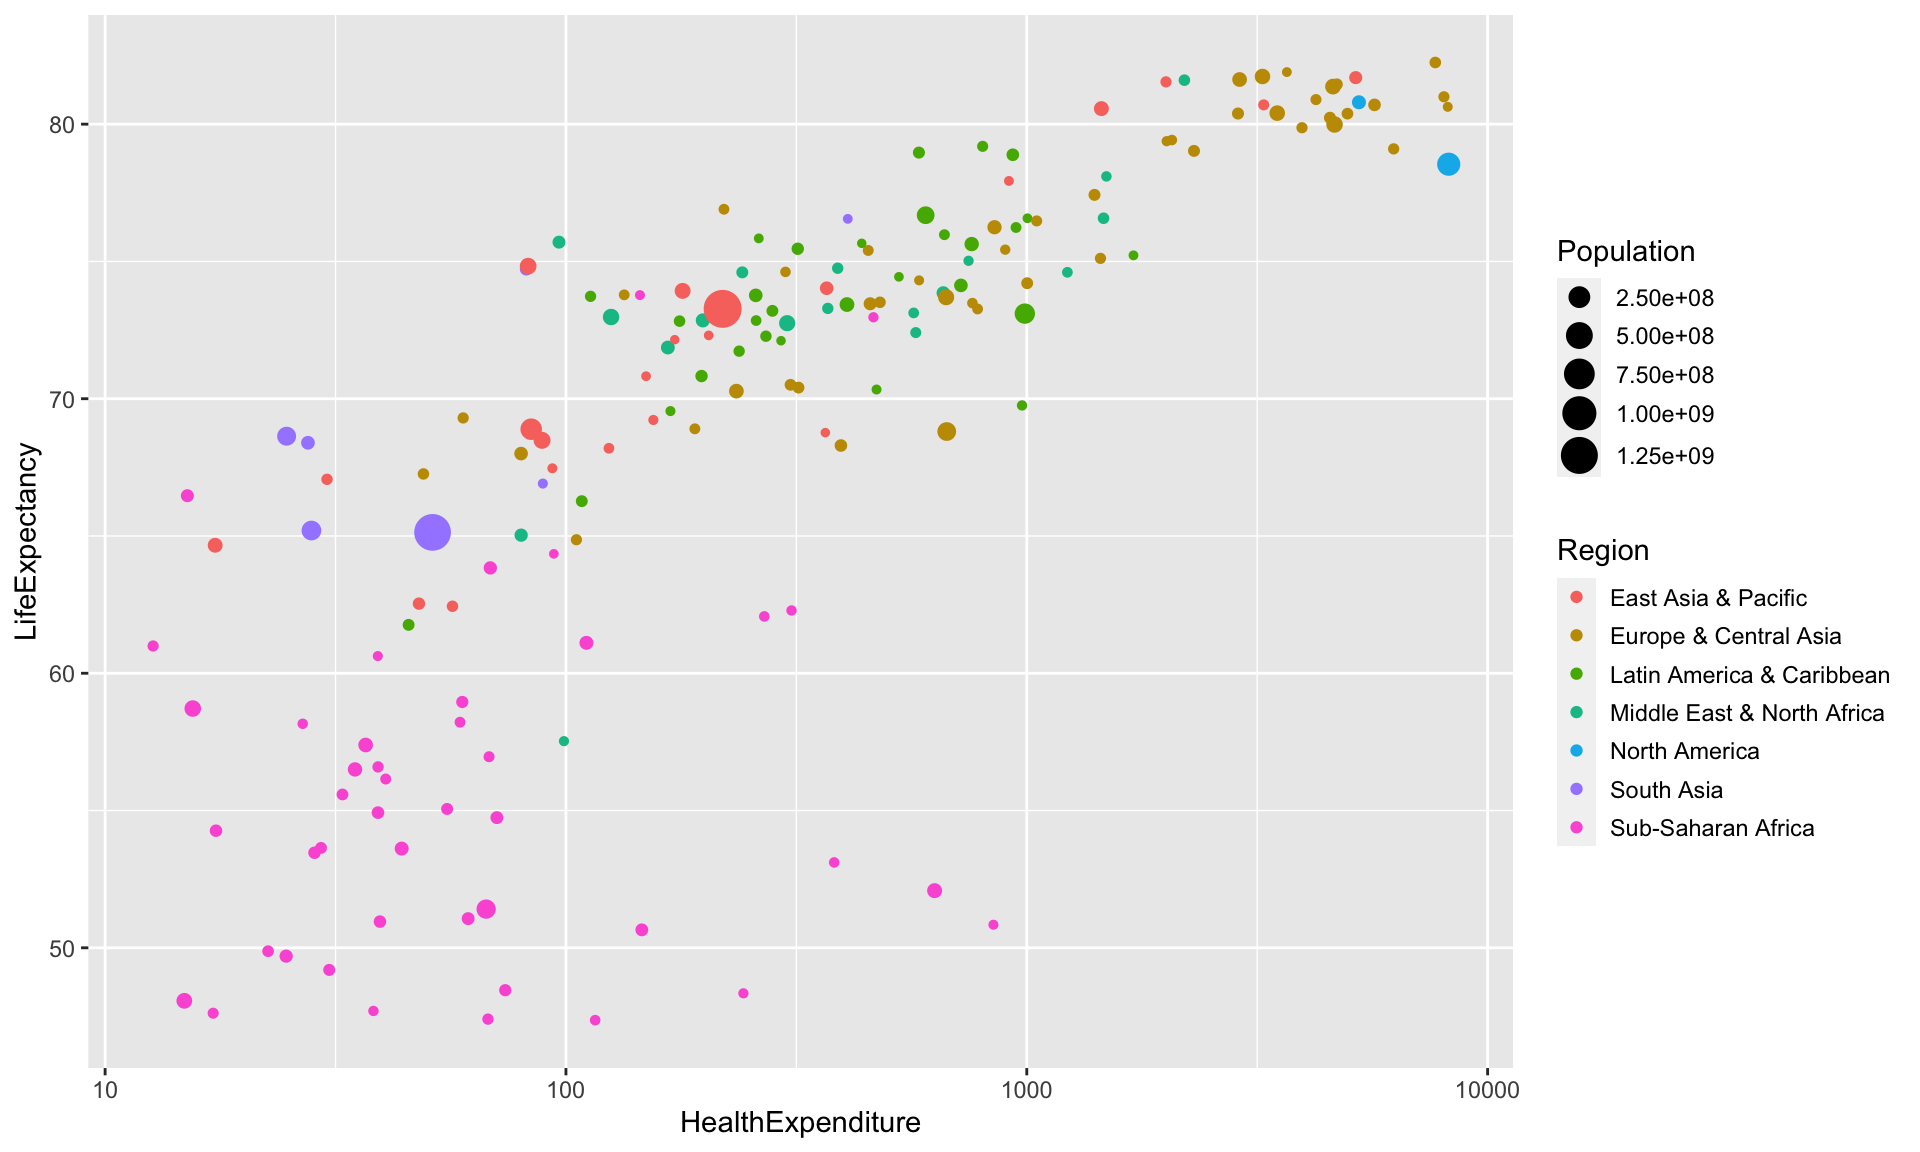
\includegraphics[width=\textwidth]{bookdown-demo_files/figure-latex/unnamed-chunk-53-1}

\hypertarget{adding-additional-layers}{%
\subsection{Adding additional layers}\label{adding-additional-layers}}

Additional layers can simply be added to the plot. For example, we can add an overall regression line with confidence bands using

\begin{Shaded}
\begin{Highlighting}[]
\FunctionTok{ggplot}\NormalTok{(}\AttributeTok{data=}\NormalTok{health) }\SpecialCharTok{+} 
    \FunctionTok{aes}\NormalTok{(}\AttributeTok{x=}\NormalTok{HealthExpenditure,  }\AttributeTok{y=}\NormalTok{LifeExpectancy) }\SpecialCharTok{+}
    \FunctionTok{geom\_point}\NormalTok{(}\FunctionTok{aes}\NormalTok{(}\AttributeTok{colour=}\NormalTok{Region, }\AttributeTok{size=}\NormalTok{Population)) }\SpecialCharTok{+}
    \FunctionTok{geom\_smooth}\NormalTok{(}\AttributeTok{method=}\StringTok{"lm"}\NormalTok{)  }\SpecialCharTok{+}
    \FunctionTok{scale\_x\_log10}\NormalTok{()}
\end{Highlighting}
\end{Shaded}

\begin{verbatim}
## `geom_smooth()` using formula 'y ~ x'
\end{verbatim}

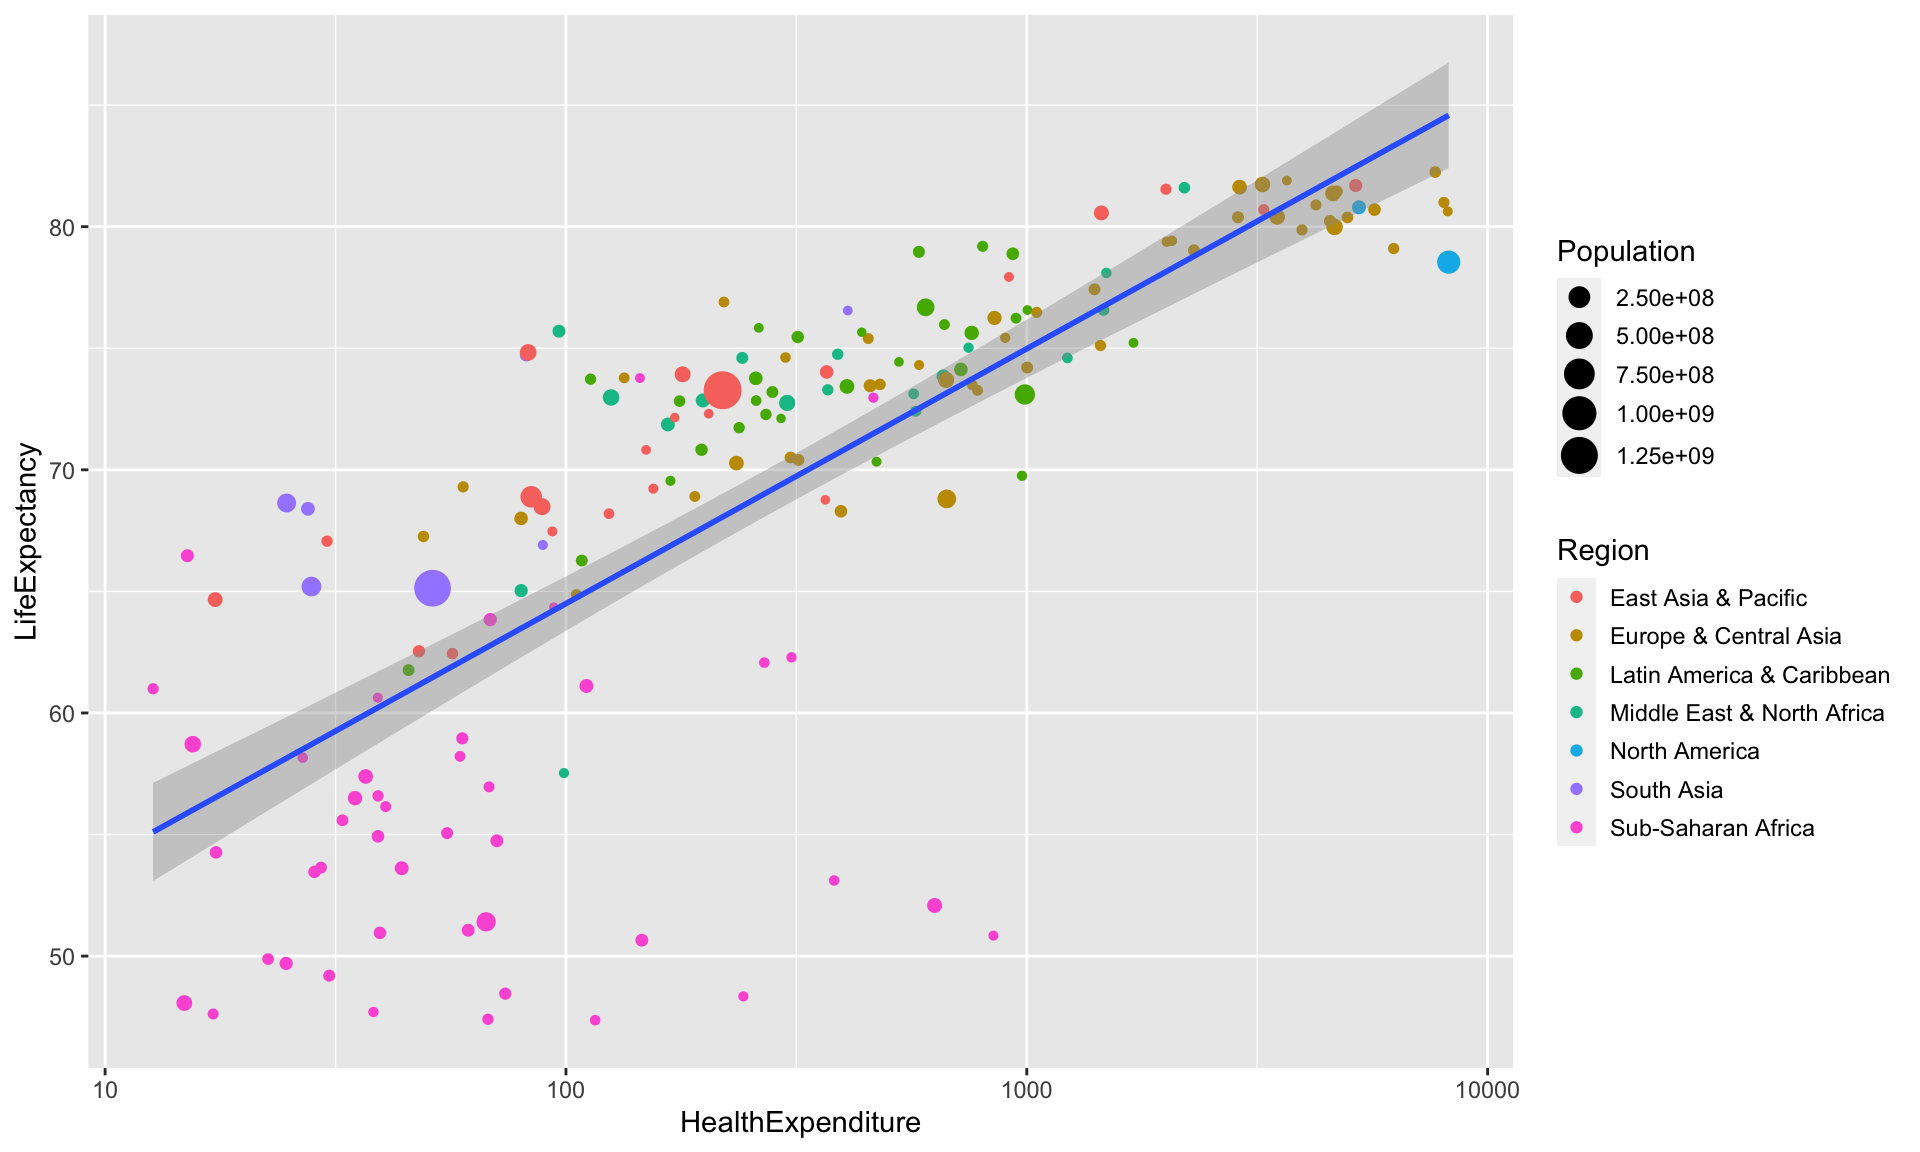
\includegraphics[width=\textwidth]{bookdown-demo_files/figure-latex/unnamed-chunk-54-1}

If we want to add a different regression line for each country we have to make sure that a \texttt{group} or \texttt{colour} aesthetic is passed to \texttt{geom\_smooth}. We could pass \texttt{aes(colour=Region)} to \texttt{geom\_smooth}. Alternatively, we can move \texttt{colour=Region} from the aesthetics specific to \texttt{geom\_point} to the generic aesthetics, so that \texttt{colour=Region} now applies to both \texttt{geom\_point} and \texttt{geom\_smooth}.

\begin{Shaded}
\begin{Highlighting}[]
\FunctionTok{ggplot}\NormalTok{(}\AttributeTok{data=}\NormalTok{health) }\SpecialCharTok{+} 
    \FunctionTok{aes}\NormalTok{(}\AttributeTok{x=}\NormalTok{HealthExpenditure,  }\AttributeTok{y=}\NormalTok{LifeExpectancy, }\AttributeTok{colour=}\NormalTok{Region) }\SpecialCharTok{+}
    \FunctionTok{geom\_point}\NormalTok{(}\FunctionTok{aes}\NormalTok{(}\AttributeTok{size=}\NormalTok{Population)) }\SpecialCharTok{+}
    \FunctionTok{geom\_smooth}\NormalTok{(}\AttributeTok{method=}\StringTok{"lm"}\NormalTok{)  }\SpecialCharTok{+}
    \FunctionTok{scale\_x\_log10}\NormalTok{()}
\end{Highlighting}
\end{Shaded}

\begin{verbatim}
## `geom_smooth()` using formula 'y ~ x'
\end{verbatim}

\begin{verbatim}
## Warning in qt((1 - level)/2, df): NaNs produced
\end{verbatim}

\begin{verbatim}
## Warning in max(ids, na.rm = TRUE): no non-missing arguments to max; returning
## -Inf
\end{verbatim}

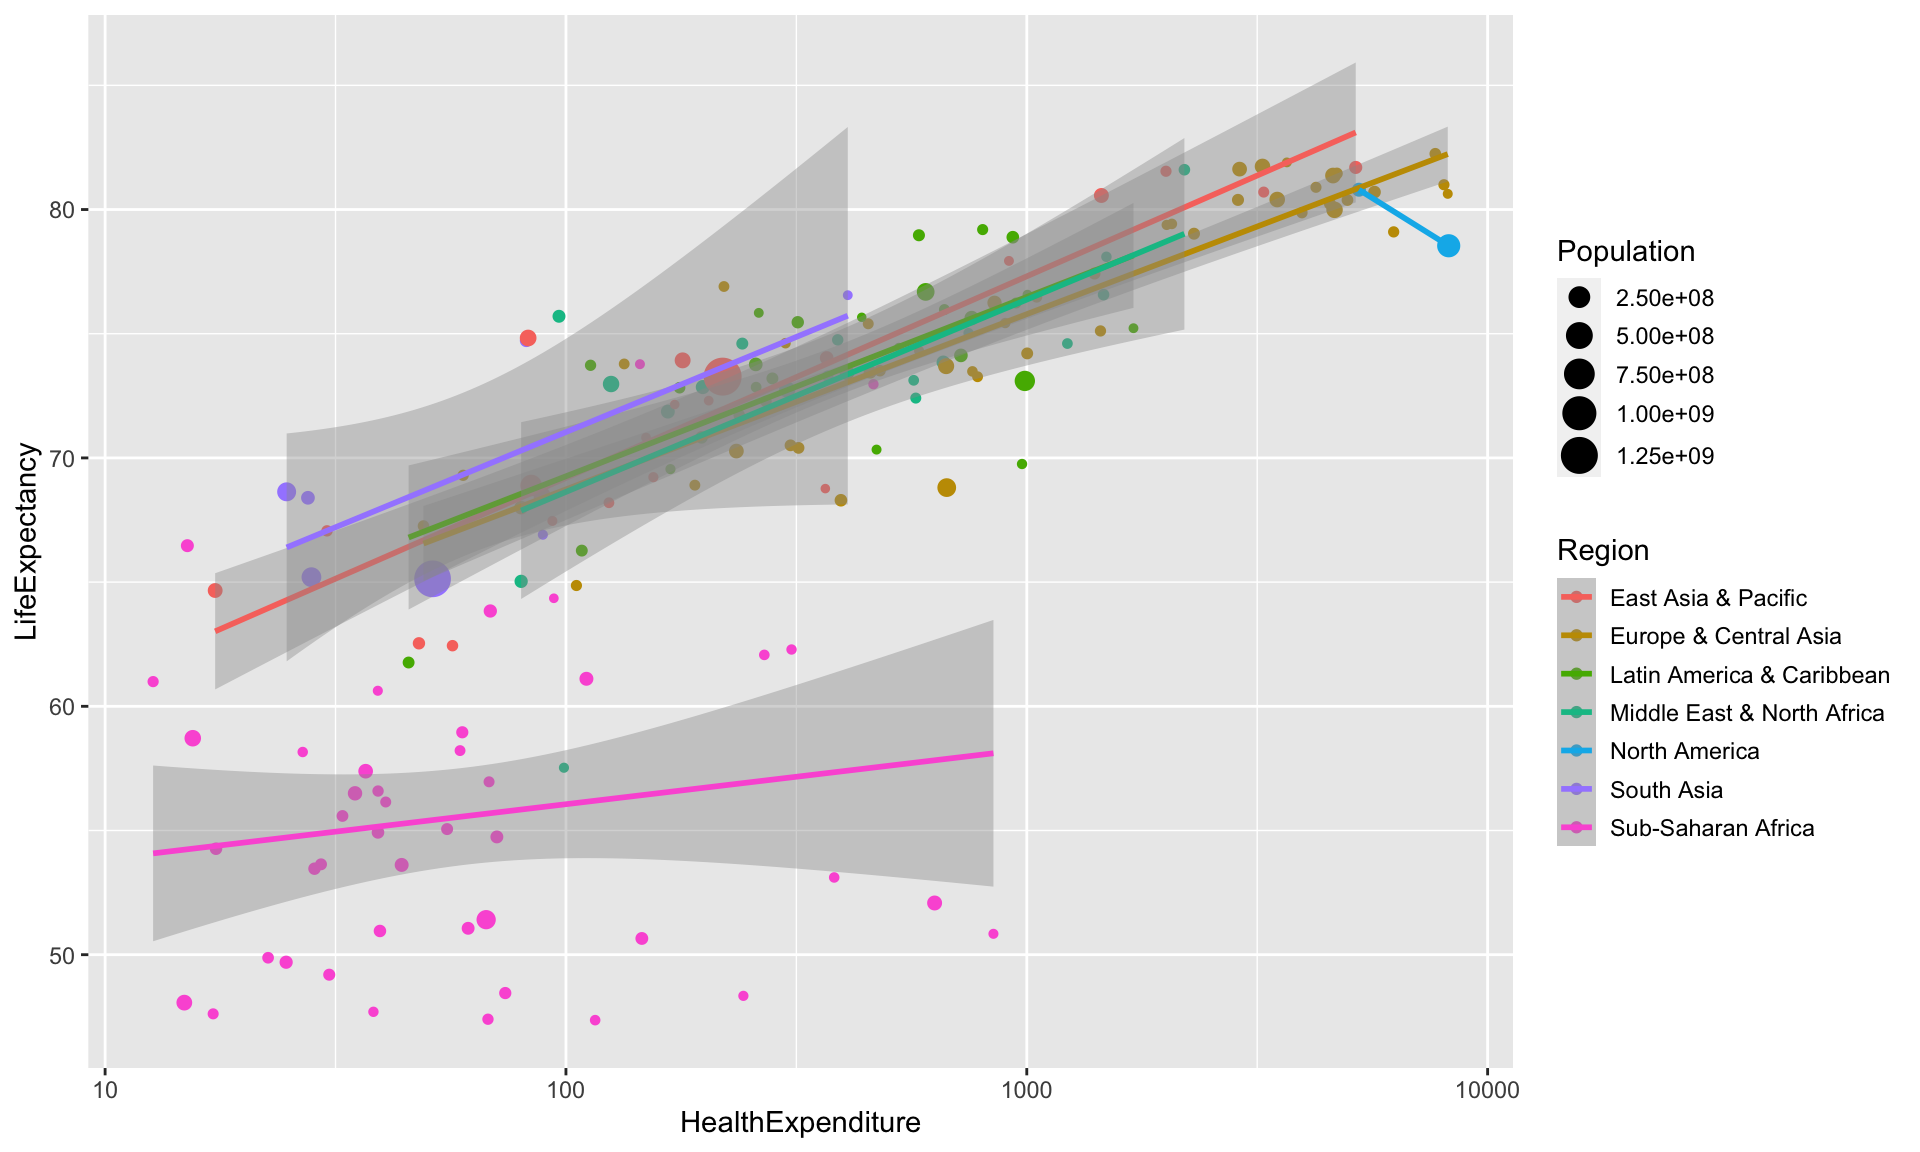
\includegraphics[width=\textwidth]{bookdown-demo_files/figure-latex/unnamed-chunk-55-1}

The warning comes from the fact that there are only two North American countries, so we can fit a line through them with no error, which means we cannot draw confidence bands.

The plot looks slightly messy, we will use \texttt{facet\_wrap} later on to split it into separate panels.

Suppose we want to annotate the observations belonging to Australia, the UK, the US.

\begin{Shaded}
\begin{Highlighting}[]
\NormalTok{health2 }\OtherTok{\textless{}{-}}\NormalTok{ health }\SpecialCharTok{\%\textgreater{}\%}
    \FunctionTok{filter}\NormalTok{(Country }\SpecialCharTok{\%in\%} \FunctionTok{c}\NormalTok{(}\StringTok{"Australia"}\NormalTok{, }\StringTok{"United Kingdom"}\NormalTok{, }\StringTok{"United States"}\NormalTok{))}
\FunctionTok{ggplot}\NormalTok{(}\AttributeTok{data=}\NormalTok{health) }\SpecialCharTok{+} 
    \FunctionTok{aes}\NormalTok{(}\AttributeTok{x=}\NormalTok{HealthExpenditure,  }\AttributeTok{y=}\NormalTok{LifeExpectancy, }\AttributeTok{colour=}\NormalTok{Region) }\SpecialCharTok{+}
    \FunctionTok{geom\_point}\NormalTok{(}\FunctionTok{aes}\NormalTok{(}\AttributeTok{size=}\NormalTok{Population)) }\SpecialCharTok{+}
    \FunctionTok{geom\_label}\NormalTok{(}\AttributeTok{data=}\NormalTok{health2, }
               \FunctionTok{aes}\NormalTok{(}\AttributeTok{x=}\NormalTok{HealthExpenditure,  }\AttributeTok{y=}\NormalTok{LifeExpectancy, }\AttributeTok{label=}\NormalTok{Country),}
               \AttributeTok{show.legend=}\ConstantTok{FALSE}\NormalTok{)}
\end{Highlighting}
\end{Shaded}

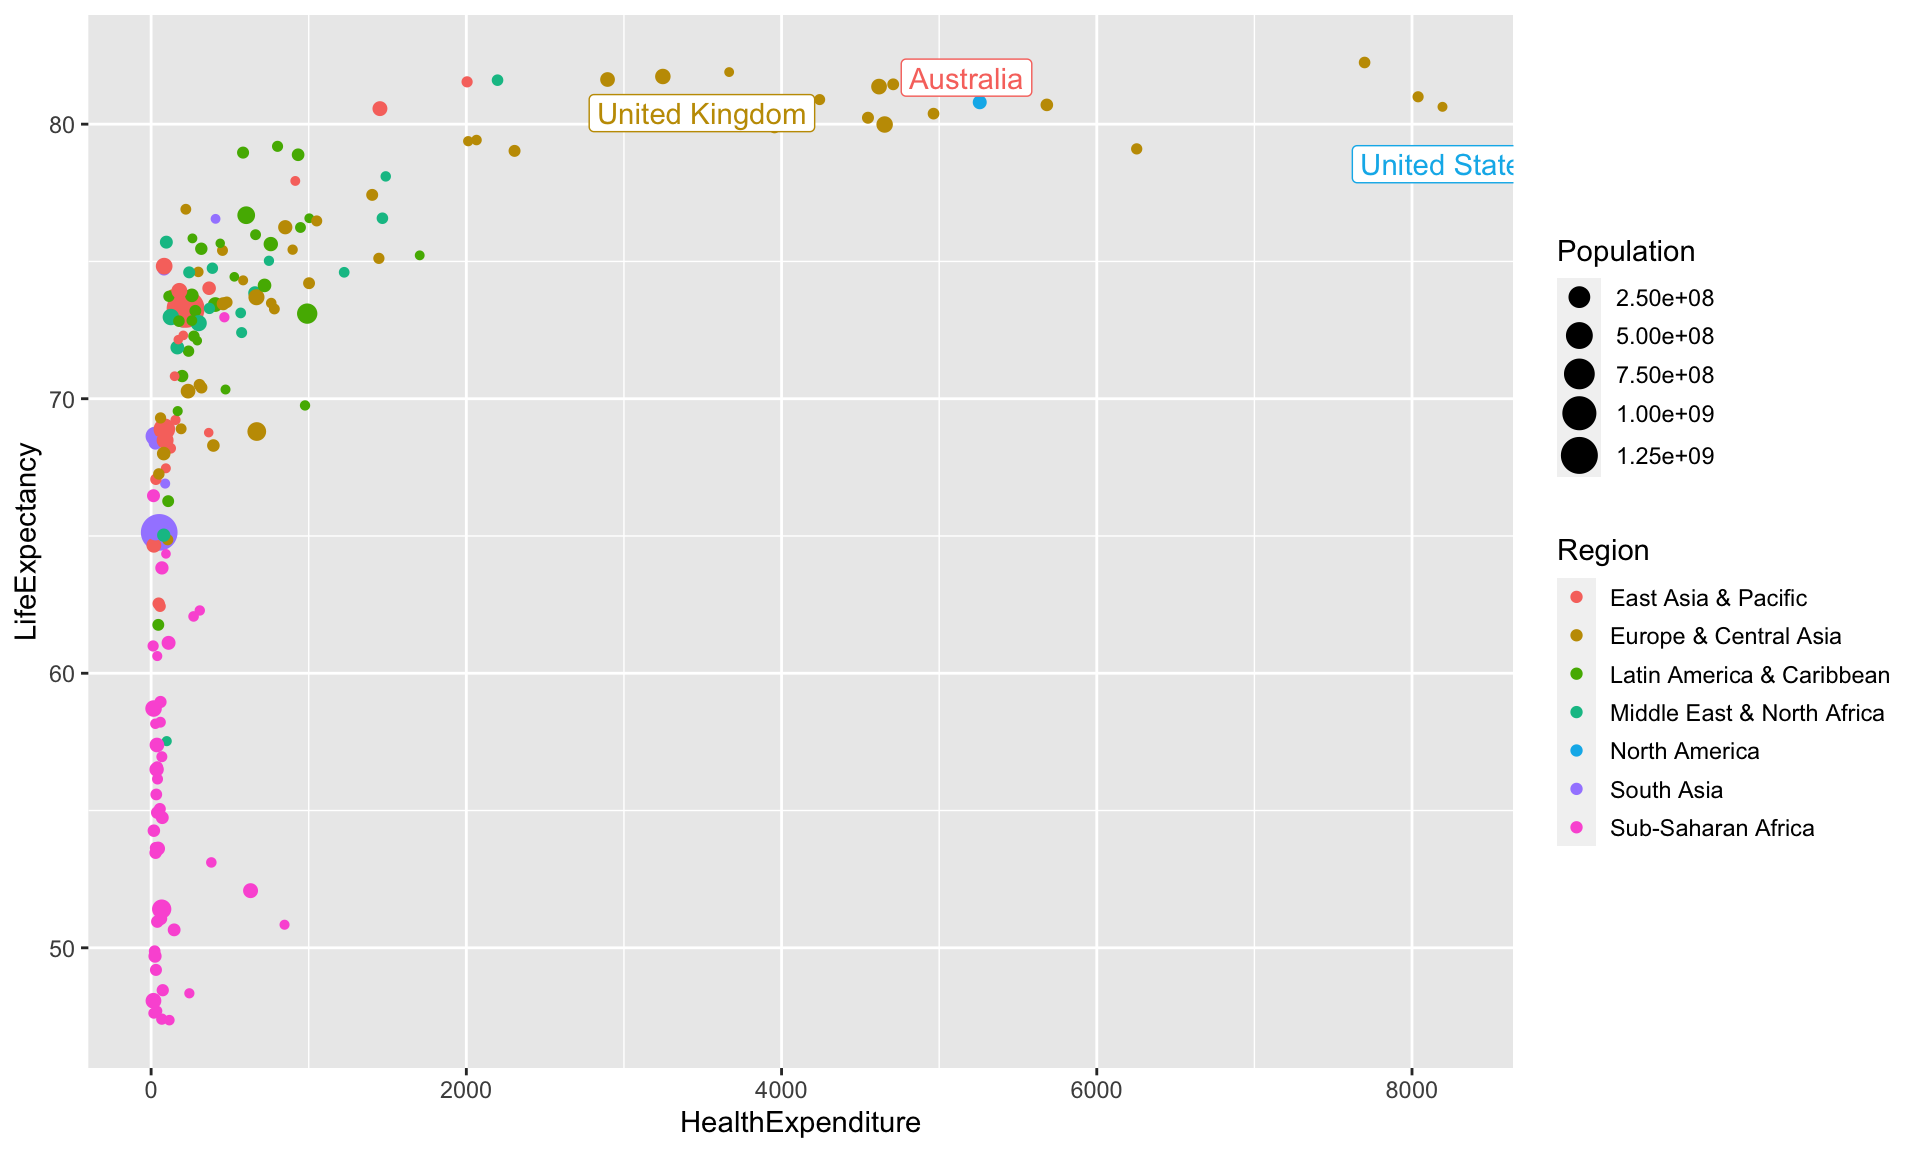
\includegraphics[width=\textwidth]{bookdown-demo_files/figure-latex/unnamed-chunk-56-1}

The labels however cover the observations and might not be fully visible. This can be avoided by using the function \texttt{geom\_label\_repel} from \href{https://cran.r-project.org/web/packages/ggrepel}{ggrepel}.

\begin{Shaded}
\begin{Highlighting}[]
\NormalTok{health }\OtherTok{\textless{}{-}}\NormalTok{ health }\SpecialCharTok{\%\textgreater{}\%}
    \FunctionTok{mutate}\NormalTok{(}\AttributeTok{CountryLabel=}\FunctionTok{ifelse}\NormalTok{(Country}\SpecialCharTok{\%in\%}\FunctionTok{c}\NormalTok{(}\StringTok{"Australia"}\NormalTok{, }\StringTok{"United Kingdom"}\NormalTok{, }\StringTok{"United States"}\NormalTok{),}
                               \FunctionTok{as.character}\NormalTok{(Country),}\StringTok{""}\NormalTok{))}

\FunctionTok{library}\NormalTok{(ggrepel)}
\FunctionTok{ggplot}\NormalTok{(}\AttributeTok{data=}\NormalTok{health) }\SpecialCharTok{+} 
    \FunctionTok{aes}\NormalTok{(}\AttributeTok{x=}\NormalTok{HealthExpenditure,  }\AttributeTok{y=}\NormalTok{LifeExpectancy, }\AttributeTok{colour=}\NormalTok{Region) }\SpecialCharTok{+}
    \FunctionTok{geom\_point}\NormalTok{(}\FunctionTok{aes}\NormalTok{(}\AttributeTok{size=}\NormalTok{Population)) }\SpecialCharTok{+}
    \FunctionTok{geom\_label\_repel}\NormalTok{(}\FunctionTok{aes}\NormalTok{(}\AttributeTok{label=}\NormalTok{CountryLabel), }\AttributeTok{show.legend=}\ConstantTok{FALSE}\NormalTok{)}
\end{Highlighting}
\end{Shaded}

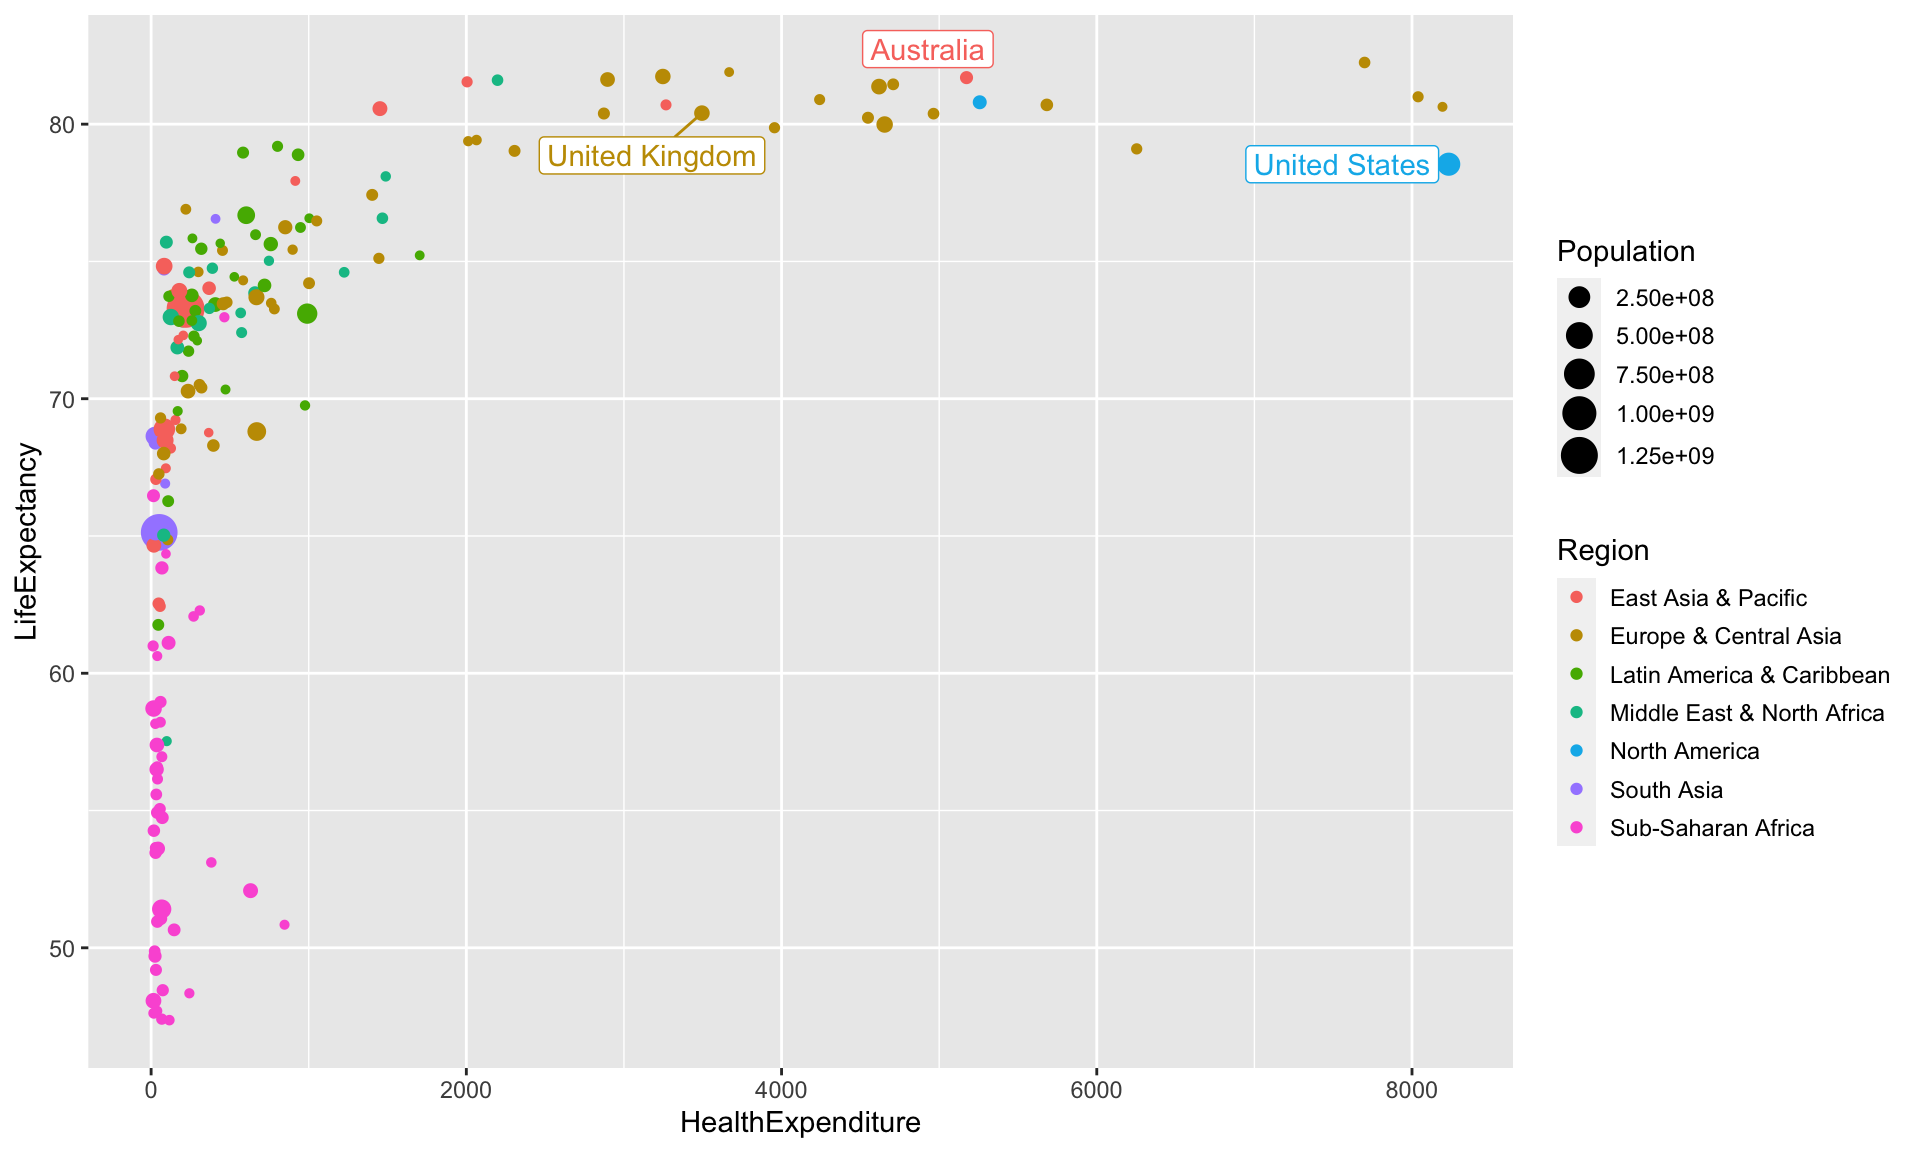
\includegraphics[width=\textwidth]{bookdown-demo_files/figure-latex/unnamed-chunk-57-1}

This time, we have used a different approach. Rather than subsetting the data and creating a separate data frame only containing the data for the three countries, we have created a new column in the data frame \texttt{health}, which is blank except for the three countries. This is required because \texttt{ggrepel} layers are only aware of data drawn in their own layer: this way we can avoid the labels covering observations we have not labelled.

\hypertarget{explicit-drawing}{%
\subsection{Explicit drawing}\label{explicit-drawing}}

The standard R plotting functions draw a plot as soon as the plot function is invoked.

Plotting commands in \texttt{ggplot2} (including \texttt{qplot}) return objects (otherwise the \texttt{+} notation would not work) and only draw the plot when their \texttt{print} or \texttt{plot} methods are invoked. In the console this is the case when they are used without an assignment.

\begin{Shaded}
\begin{Highlighting}[]
\NormalTok{a }\OtherTok{\textless{}{-}} \FunctionTok{ggplot}\NormalTok{(}\AttributeTok{data=}\NormalTok{health) }\SpecialCharTok{+}            \CommentTok{\# Does not draw anything}
         \FunctionTok{aes}\NormalTok{(}\AttributeTok{x=}\NormalTok{HealthExpenditure, }\AttributeTok{y=}\NormalTok{LifeExpectancy) }\SpecialCharTok{+}
         \FunctionTok{geom\_point}\NormalTok{()}

\NormalTok{b }\OtherTok{\textless{}{-}}\NormalTok{ a }\SpecialCharTok{+} \FunctionTok{scale\_x\_log10}\NormalTok{()              }\CommentTok{\# Does not draw anything either}

\NormalTok{a                                     }\CommentTok{\# Now the plot stored in a gets drawn}
\FunctionTok{print}\NormalTok{(a)                              }\CommentTok{\# Draw a again (explicit invocation)}

\NormalTok{b                                     }\CommentTok{\# Now the plot stored in b gets drawn}
\end{Highlighting}
\end{Shaded}

Inside loops and functions the \texttt{print} or \texttt{plot} methods need to be invoked explicitly by using the methods \texttt{print} or \texttt{plot}.

\hypertarget{task-7}{%
\subsection{Task}\label{task-7}}

Consider two vectors \texttt{x} and \texttt{y} created using

\begin{Shaded}
\begin{Highlighting}[]
\NormalTok{n }\OtherTok{\textless{}{-}} \FloatTok{1e3}
\NormalTok{x }\OtherTok{\textless{}{-}} \FunctionTok{runif}\NormalTok{(n, }\DecValTok{0}\NormalTok{, }\DecValTok{2}\SpecialCharTok{*}\NormalTok{pi)                   }\CommentTok{\# x is random uniform from (0,2*pi)}
\CommentTok{\# x \textless{}{-} sort(x)                           \# Sorting of x \_not\_ needed for ggplot}
\NormalTok{y }\OtherTok{\textless{}{-}} \FunctionTok{sin}\NormalTok{(x)                              }\CommentTok{\# Set y to the sine of x}
\NormalTok{y.noisy }\OtherTok{\textless{}{-}}\NormalTok{ y }\SpecialCharTok{+}\NormalTok{ .}\DecValTok{25} \SpecialCharTok{*} \FunctionTok{rnorm}\NormalTok{(n)            }\CommentTok{\# Create noisy version of y}
\end{Highlighting}
\end{Shaded}

Use \texttt{ggplot2} to create a scatterplot of \texttt{y.noisy} against \texttt{x}, which also shows the noise-free sine curve in \texttt{y}.

\hypertarget{answer-6}{%
\subsection{Answer}\label{answer-6}}

We can use the following R code:

\begin{Shaded}
\begin{Highlighting}[]
\FunctionTok{ggplot}\NormalTok{() }\SpecialCharTok{+}                               \CommentTok{\# No need to use data=... as x, y and y.noisy}
                                         \CommentTok{\# are variables in the workspace and not columns}
                                         \CommentTok{\# in a dataset}
    \FunctionTok{geom\_point}\NormalTok{(}\FunctionTok{aes}\NormalTok{(x, y.noisy)) }\SpecialCharTok{+}
    \FunctionTok{geom\_line}\NormalTok{(}\FunctionTok{aes}\NormalTok{(x, y))}
\end{Highlighting}
\end{Shaded}

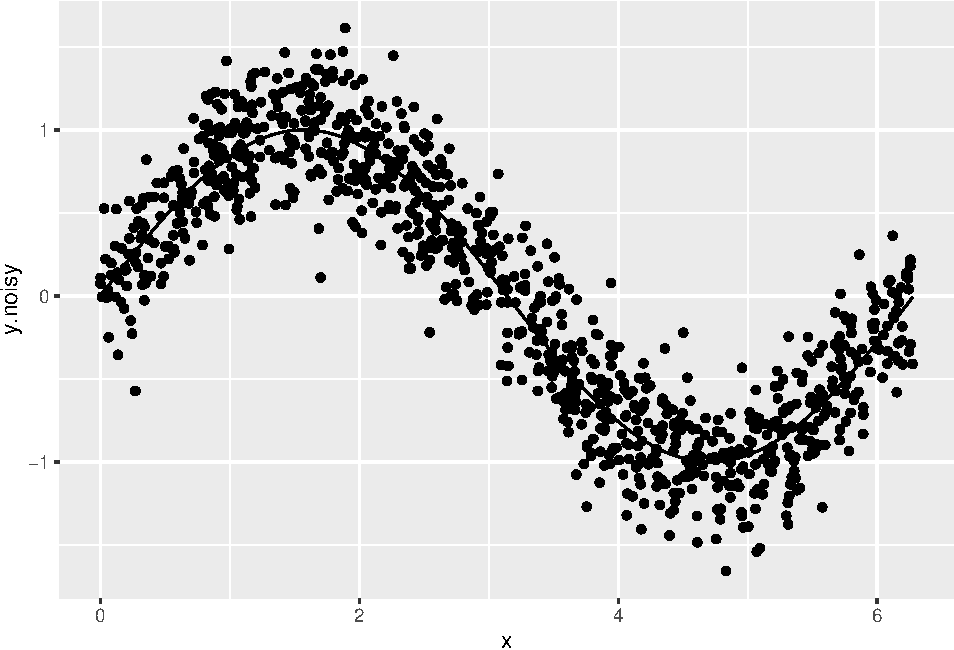
\includegraphics{bookdown-demo_files/figure-latex/unnamed-chunk-59-1.pdf}

It does not matter whether \texttt{geom\_point} or \texttt{geom\_line} comes first. \texttt{ggplot2} adapts the axes so that all objects drawn fit (and not just the first one as is the case when using standard R plotting functions \texttt{plot} and \texttt{points}).

\hypertarget{modifying-plots}{%
\section{Modifying Plots}\label{modifying-plots}}

\hypertarget{labels-and-titles}{%
\subsection{Labels and titles}\label{labels-and-titles}}

We can set the plot title using \texttt{ggtitle(title)} and the axis labels using \texttt{xlab(label)} and \texttt{ylab(label)}.

\begin{Shaded}
\begin{Highlighting}[]
\FunctionTok{ggplot}\NormalTok{(}\AttributeTok{data=}\NormalTok{health) }\SpecialCharTok{+} 
    \FunctionTok{aes}\NormalTok{(}\AttributeTok{x=}\NormalTok{HealthExpenditure,  }\AttributeTok{y=}\NormalTok{LifeExpectancy, }\AttributeTok{colour=}\NormalTok{Region) }\SpecialCharTok{+}
    \FunctionTok{geom\_point}\NormalTok{(}\FunctionTok{aes}\NormalTok{(}\AttributeTok{size=}\NormalTok{Population)) }\SpecialCharTok{+}
    \FunctionTok{geom\_smooth}\NormalTok{(}\AttributeTok{method=}\StringTok{"lm"}\NormalTok{)  }\SpecialCharTok{+}
    \FunctionTok{scale\_x\_log10}\NormalTok{() }\SpecialCharTok{+}
    \FunctionTok{ggtitle}\NormalTok{(}\StringTok{"Relationship between Health Expenditure and Life Expectancy"}\NormalTok{) }\SpecialCharTok{+}
    \FunctionTok{xlab}\NormalTok{(}\StringTok{"Health Expenditure"}\NormalTok{) }\SpecialCharTok{+}
    \FunctionTok{ylab}\NormalTok{(}\StringTok{"Life Expectancy"}\NormalTok{)    }
\end{Highlighting}
\end{Shaded}

\begin{verbatim}
## `geom_smooth()` using formula 'y ~ x'
\end{verbatim}

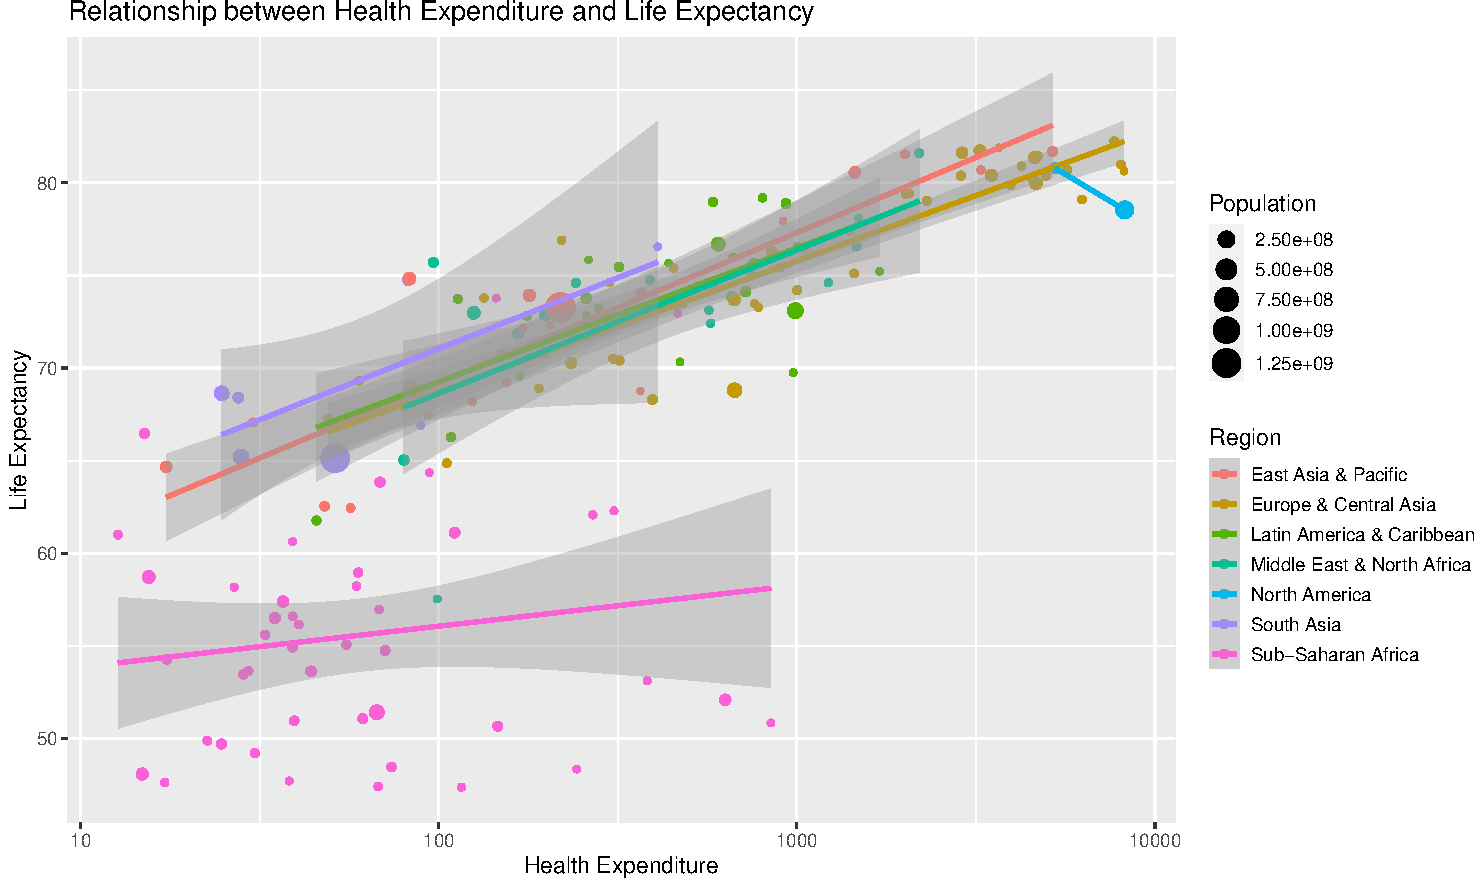
\includegraphics[width=\textwidth]{bookdown-demo_files/figure-latex/unnamed-chunk-60-1}

Changing the text shown in legends (like in our case the names of the regions) is more complicated. It is almost always easier to simply change the levels of the categorical variable in the dataset itself before invoking \texttt{ggplot2} commands.

\hypertarget{scales}{%
\subsection{Scales}\label{scales}}

Aesthetics control \emph{which} variables are mapped to \emph{which} property of the geometric object. However, aesthetics do not specify \emph{how} this mapping is performed. This is where scales come into play. Scales control \emph{how} any value from the variable is translated into a property of a geometric object: scales control for example how a variable is translated into coordinates (say through a log transform) or into colours (say though a discrete colour palette).

\texttt{ggplot2} automatically chooses (what it thinks is) a suitable scale. This is usually reasonable, but on occasions it might be necessary to override this.

There is a family of scale functions for each aesthetic. The template for the function name for scales is \texttt{scale\_\textless{}aesthetic\textgreater{}\_\textless{}type\textgreater{}}.

\hypertarget{scales-for-continuous-data}{%
\subsubsection{Scales for continuous data}\label{scales-for-continuous-data}}

We have already seen that we can log-transform the axes using \texttt{scale\_x\_log10} and \texttt{scale\_x\_log10}. The more general functions for coordinate transforms are \texttt{scale\_\textless{}x\ or\ y\textgreater{}\_continous(...)}. We can. amongst others, set the axis label (argument \texttt{name}, the ticks and tickmarks (arguments \texttt{breaks} and \texttt{labels}) the limits (argument \texttt{limit}) and the transform to be used (argument \texttt{trans}).

The axes might use scientific notation (e.g.~``4e5''). If you want to avoid using scientific notation and use fixed notation, change the \texttt{scipen} option in R, which controls when scientific notation is used (for example run \texttt{options(scipen=1e3)}).

There are functions for mapping continuous data to other aesthetics, too. For example, \texttt{scale\_colour\_gradient} converts a continuous variable to a colour using a gradient of colours. The arguments \texttt{low} and \texttt{high} specify the colours used at the two ends. \texttt{scale\_colour\_gradient2} allows for also specifying a mid-point colour (argument \texttt{mid}). \texttt{scale\_colour\_gradientn} is the most general function it allows specifying a vector of colours and corresponding vector of colours. The function \texttt{scale\_colour\_distiller} uses the colour brewer available at \href{colorbrewer.org}{http://colorbrewer2.org/} and allows for constructing colours scales which are photocopier-safe and/or work for colour-blind readers.

\begin{Shaded}
\begin{Highlighting}[]
\NormalTok{a }\OtherTok{\textless{}{-}} \FunctionTok{ggplot}\NormalTok{(}\AttributeTok{data=}\NormalTok{health) }\SpecialCharTok{+}
         \FunctionTok{aes}\NormalTok{(}\AttributeTok{x=}\NormalTok{HealthExpenditure, }\AttributeTok{y=}\NormalTok{LifeExpectancy) }\SpecialCharTok{+}
         \FunctionTok{geom\_point}\NormalTok{(}\FunctionTok{aes}\NormalTok{(}\AttributeTok{colour=}\NormalTok{Population)) }\SpecialCharTok{+}
         \FunctionTok{scale\_colour\_distiller}\NormalTok{(}\AttributeTok{palette=}\StringTok{"YlOrRd"}\NormalTok{ , }\AttributeTok{trans=}\StringTok{"log"}\NormalTok{)}
\NormalTok{a}
\end{Highlighting}
\end{Shaded}

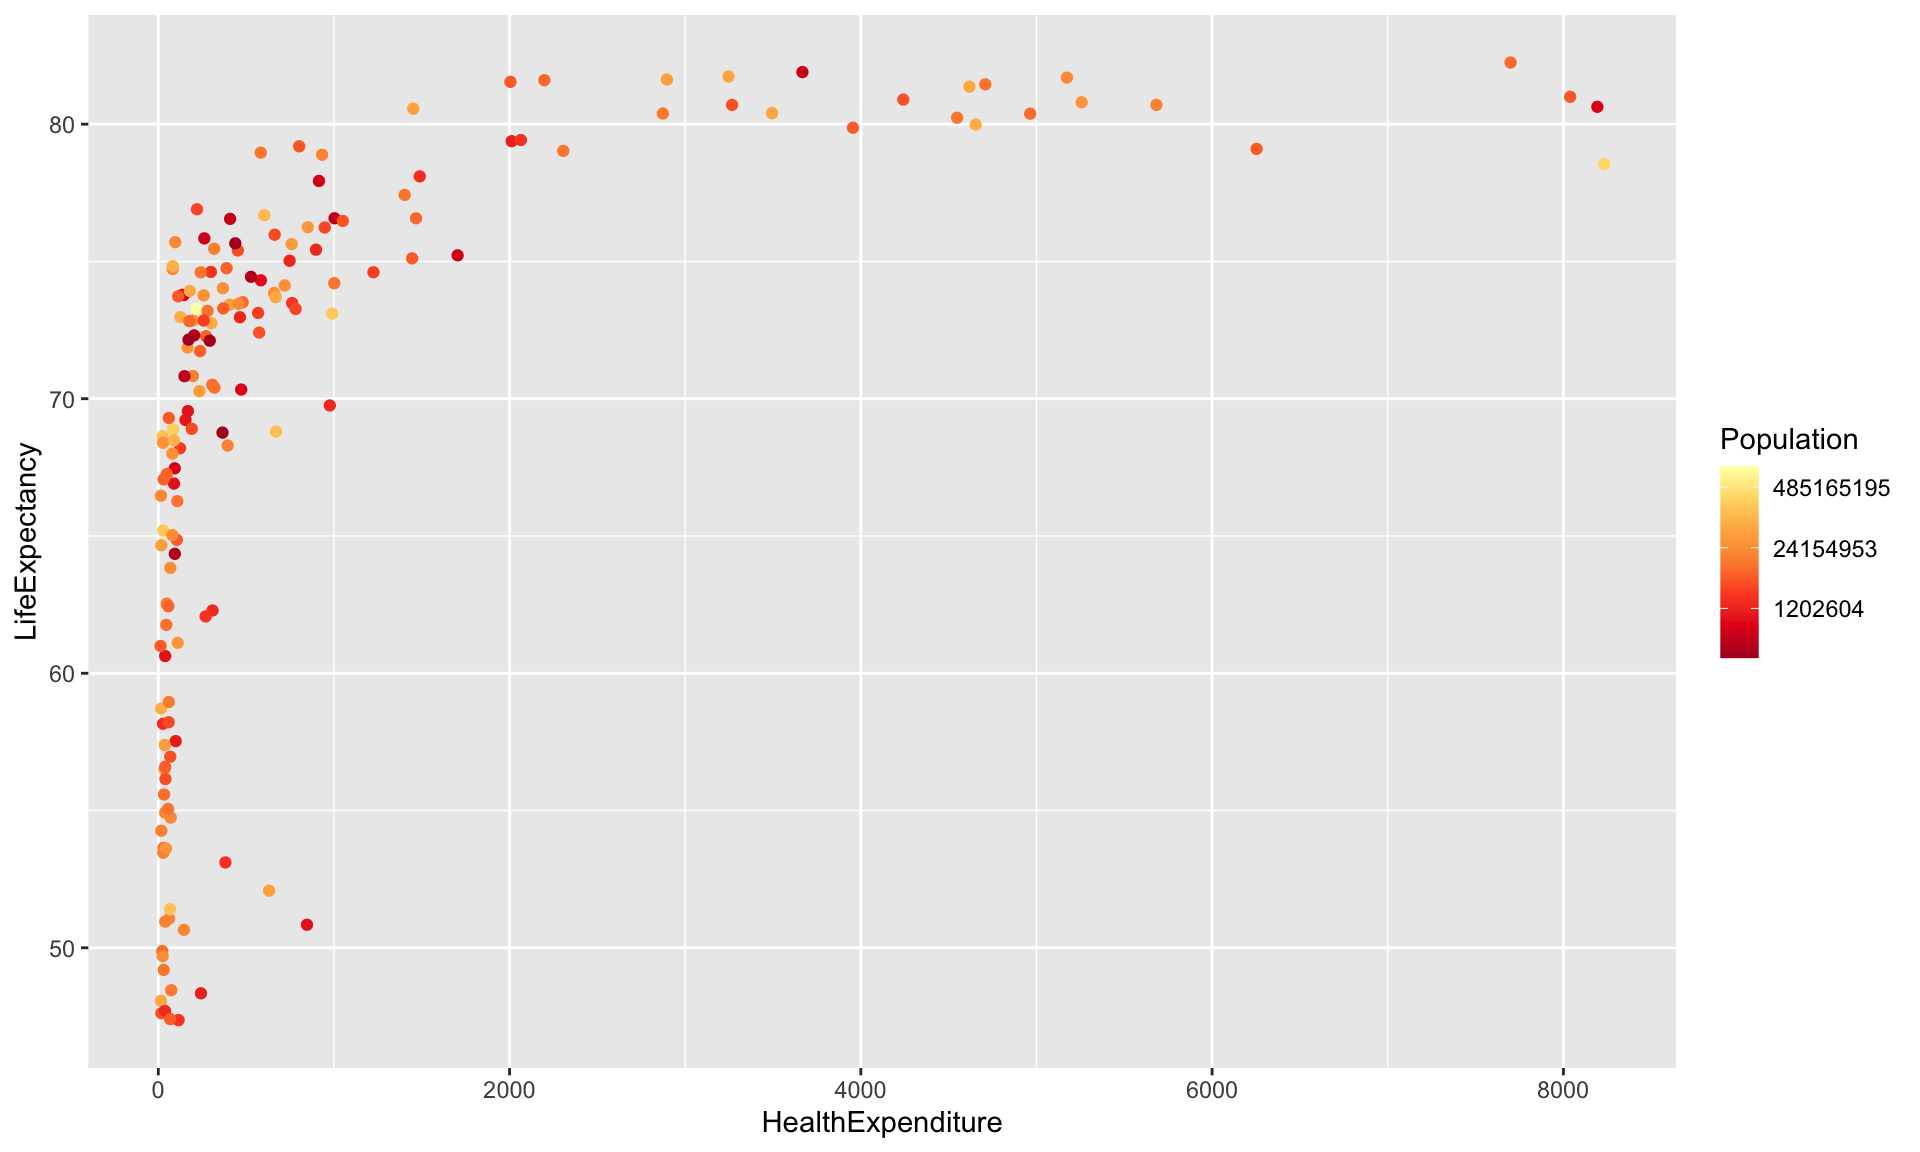
\includegraphics[width=\textwidth]{bookdown-demo_files/figure-latex/unnamed-chunk-61-1}

We have used \texttt{trans="log"} to use the log-transformed values of the population sizes (due to its skewness). The values given in the legend seem slightly odd choices: this is due to the log-transform (they are roughly \(\exp(14)\), \(\exp(17)\) and \(\exp(20)\), so ``nice'' numbers on the log scale).

We have stored the plot in a variable \texttt{a} so that we can redraw it later on with different themes.

\hypertarget{scales-for-discrete-data}{%
\subsubsection{Scales for discrete data}\label{scales-for-discrete-data}}

There are also various scaling functions for discrete data, such as \texttt{scale\_colour\_brewer}.

Note that there are separate scales for colour (outline colour -- example: \texttt{scale\_colour\_brewer}) and fill (fill colour -- example: \texttt{scale\_fill\_brewer}).

\hypertarget{statistics}{%
\subsection{Statistics}\label{statistics}}

Sometimes data has to be aggregated before it can be used in a plot. For example, when creating a bar plot illustrating the distribution of a categorical variable we have to count how many observations there are in each category. This will then determine the height of the bars. \texttt{ggplot2} automatically chooses (what it thinks is) a suitable statistic.

For example, when we draw a bar plot using \texttt{geom\_bar}, it uses by default the statistic \texttt{count}, which first produces a tally. We don't need to worry about this, \texttt{ggplot2} does all the work for us.

\begin{Shaded}
\begin{Highlighting}[]
\FunctionTok{ggplot}\NormalTok{(}\AttributeTok{data=}\NormalTok{health) }\SpecialCharTok{+}
    \FunctionTok{geom\_bar}\NormalTok{(}\FunctionTok{aes}\NormalTok{(}\AttributeTok{x=}\NormalTok{Region)) }\SpecialCharTok{+}
    \FunctionTok{theme}\NormalTok{(}\AttributeTok{axis.text.x =} \FunctionTok{element\_text}\NormalTok{(}\AttributeTok{angle =} \DecValTok{90}\NormalTok{, }\AttributeTok{hjust =} \DecValTok{1}\NormalTok{)) }\CommentTok{\# Rotate x axis labels}
\end{Highlighting}
\end{Shaded}

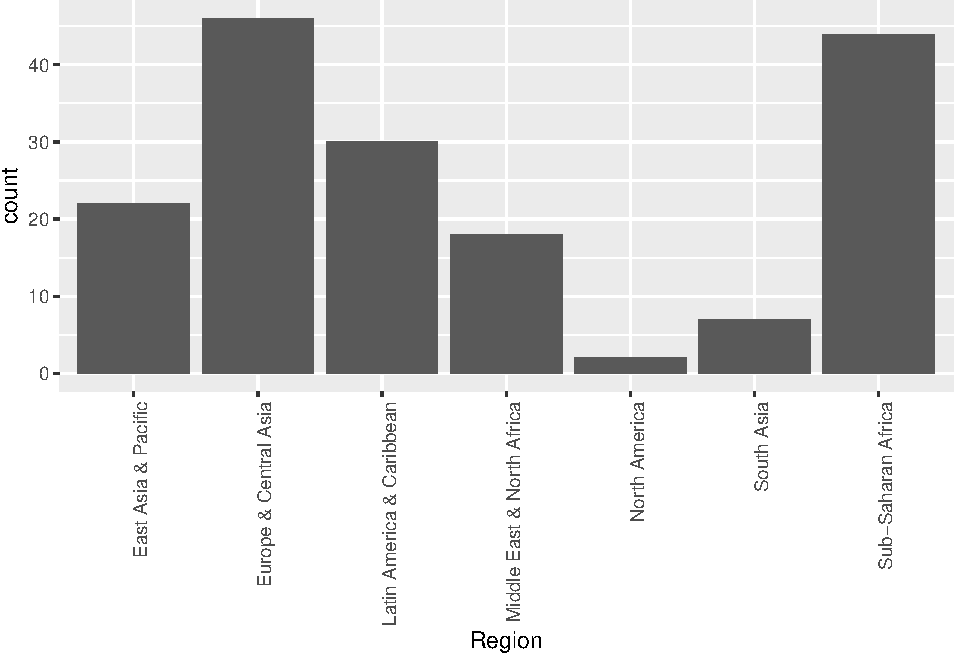
\includegraphics{bookdown-demo_files/figure-latex/unnamed-chunk-62-1.pdf}

Suppose we now want to a draw bar chart visualising the mean health expenditure in each region. Now we don't want \texttt{ggplot2} to produce a tally of how often which value occurs, we want it to simply draw the bars to the heights specified in the data. Because we now want no aggregation, we have to use the statistic \texttt{identity}.

\begin{Shaded}
\begin{Highlighting}[]
\FunctionTok{library}\NormalTok{(dplyr)}
\NormalTok{HESummary }\OtherTok{\textless{}{-}}\NormalTok{ health }\SpecialCharTok{\%\textgreater{}\%}                                      \CommentTok{\# Get avg health exp}
                 \FunctionTok{group\_by}\NormalTok{(Region) }\SpecialCharTok{\%\textgreater{}\%} 
                 \FunctionTok{summarise}\NormalTok{(}\AttributeTok{HealthExpenditure=}\FunctionTok{mean}\NormalTok{(HealthExpenditure))}
\FunctionTok{ggplot}\NormalTok{(}\AttributeTok{data=}\NormalTok{HESummary) }\SpecialCharTok{+}
    \FunctionTok{geom\_bar}\NormalTok{(}\FunctionTok{aes}\NormalTok{(}\AttributeTok{x=}\NormalTok{Region, }\AttributeTok{y=}\NormalTok{HealthExpenditure), }\AttributeTok{stat=}\StringTok{"identity"}\NormalTok{) }\SpecialCharTok{+}
    \FunctionTok{theme}\NormalTok{(}\AttributeTok{axis.text.x =} \FunctionTok{element\_text}\NormalTok{(}\AttributeTok{angle =} \DecValTok{90}\NormalTok{, }\AttributeTok{hjust =} \DecValTok{1}\NormalTok{)) }\CommentTok{\# Rotate x axis labels}
\end{Highlighting}
\end{Shaded}

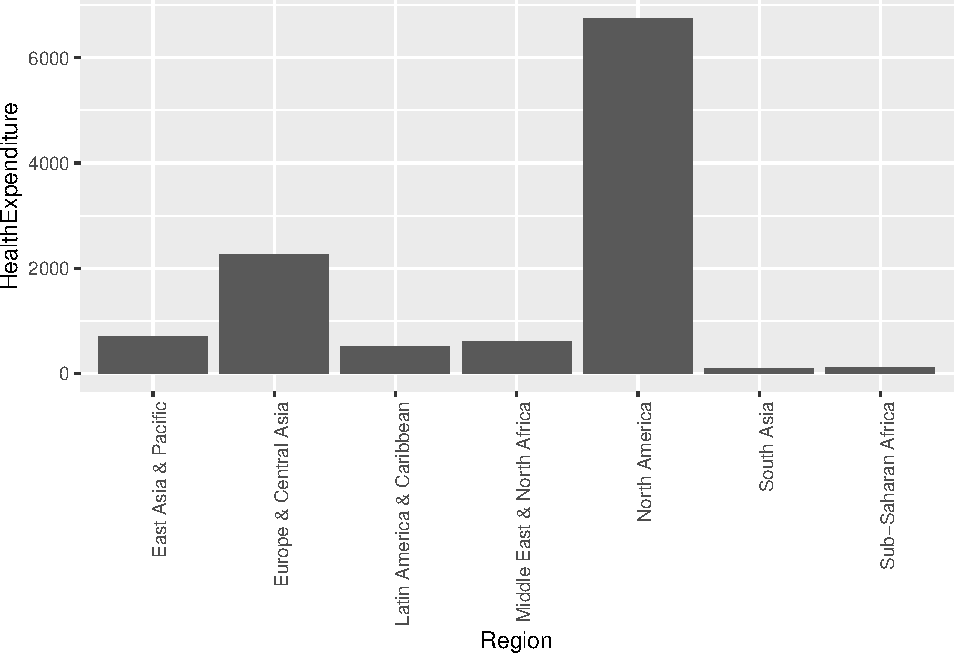
\includegraphics{bookdown-demo_files/figure-latex/unnamed-chunk-63-1.pdf}

\hypertarget{theming}{%
\subsection{Theming}\label{theming}}

Themes can be used to customise how \texttt{ggplot2} graphics look like. We have already used \texttt{theme} to change how the horizontal axis is typeset.

\texttt{ggplot2} has several themes built-in. The default theme is \texttt{theme\_gray}. Other themes available are \texttt{theme\_bw} (monochrome), \texttt{theme\_light}, \texttt{theme\_lindedraw} and \texttt{theme\_minimal}. Further themes are available in extension packages such \href{https://cran.r-project.org/web/packages/ggthemes}{ggthemes}.

\begin{Shaded}
\begin{Highlighting}[]
\NormalTok{a }\SpecialCharTok{+} \FunctionTok{theme\_minimal}\NormalTok{()}
\end{Highlighting}
\end{Shaded}

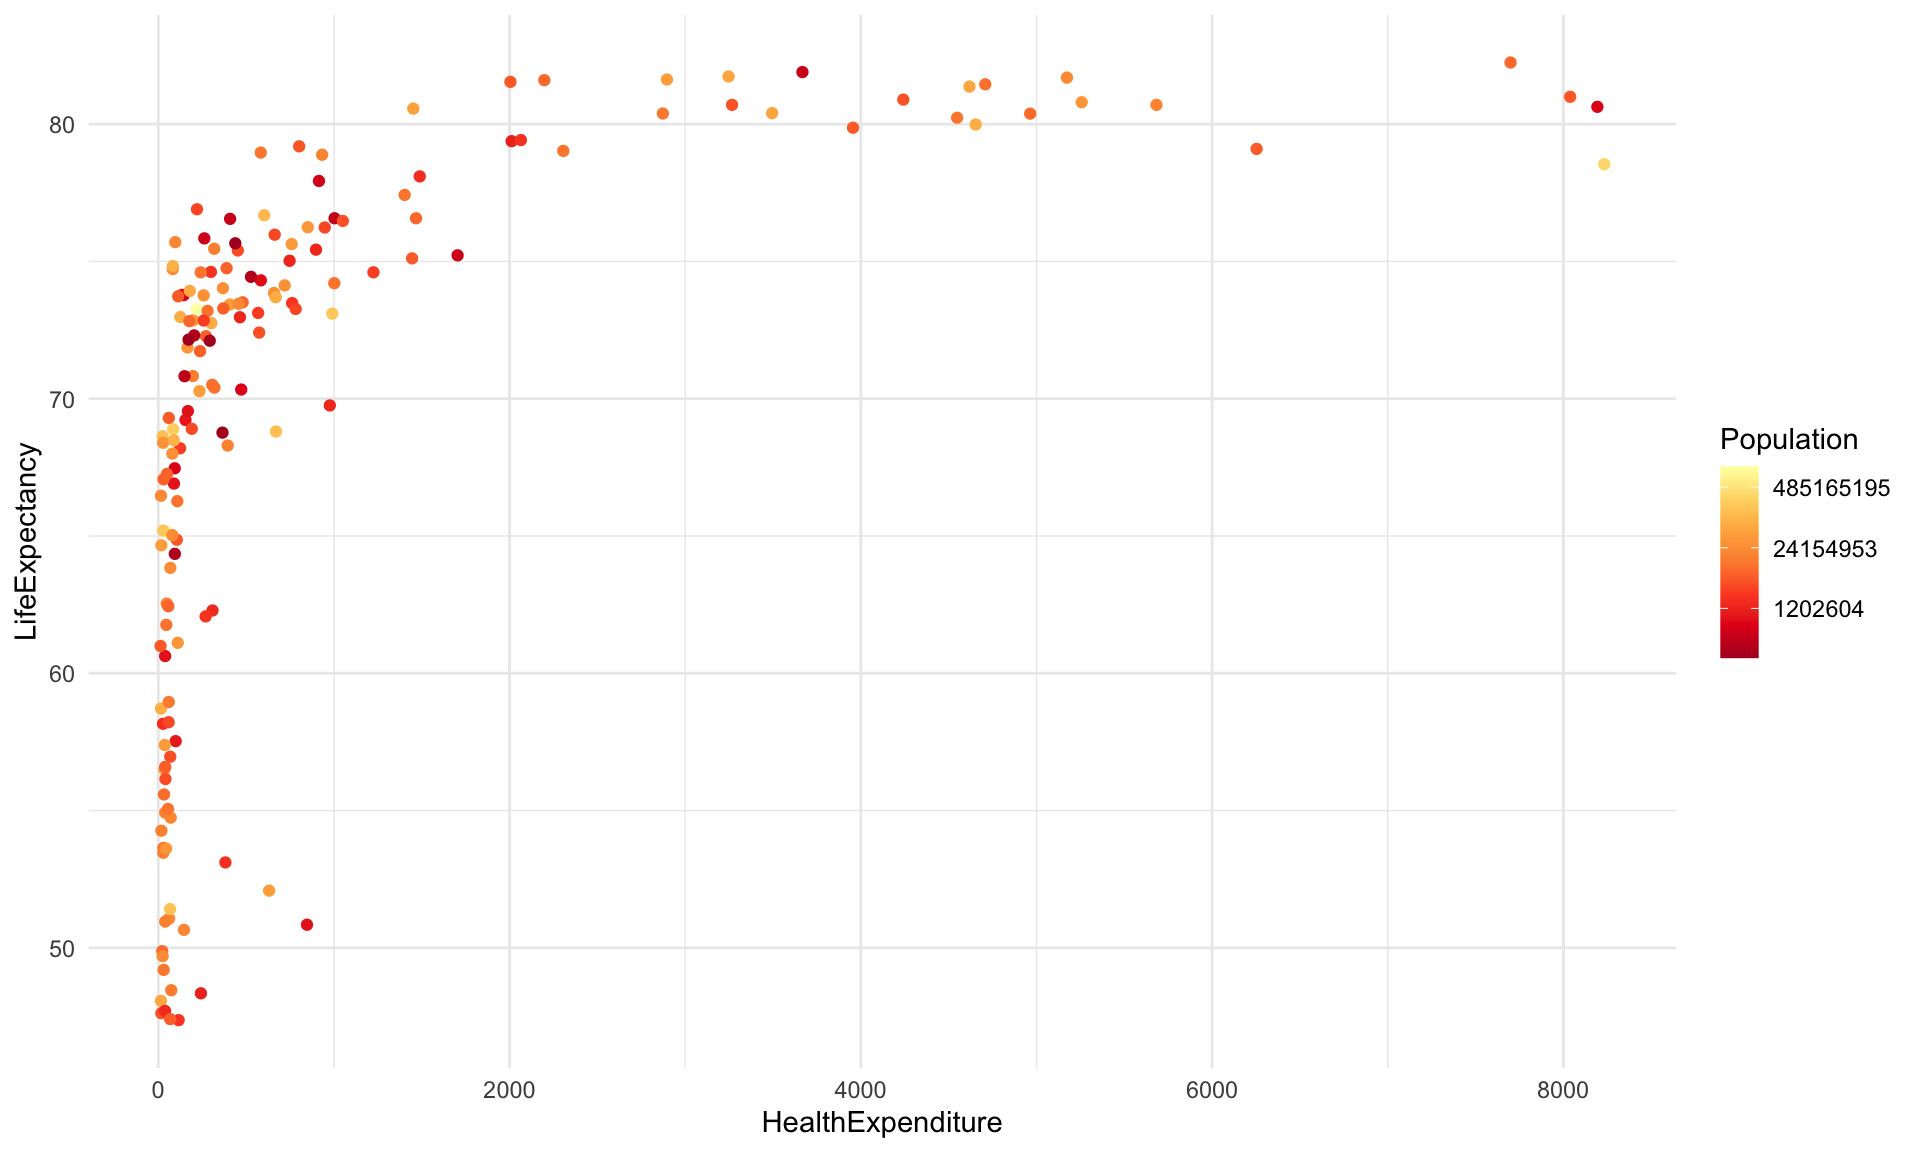
\includegraphics[width=\textwidth]{bookdown-demo_files/figure-latex/unnamed-chunk-64-1}

\begin{Shaded}
\begin{Highlighting}[]
\FunctionTok{library}\NormalTok{(ggthemes)}
\NormalTok{a }\SpecialCharTok{+} \FunctionTok{theme\_economist}\NormalTok{() }\SpecialCharTok{+} \FunctionTok{theme}\NormalTok{(}\AttributeTok{legend.position=}\StringTok{"right"}\NormalTok{)}
\end{Highlighting}
\end{Shaded}

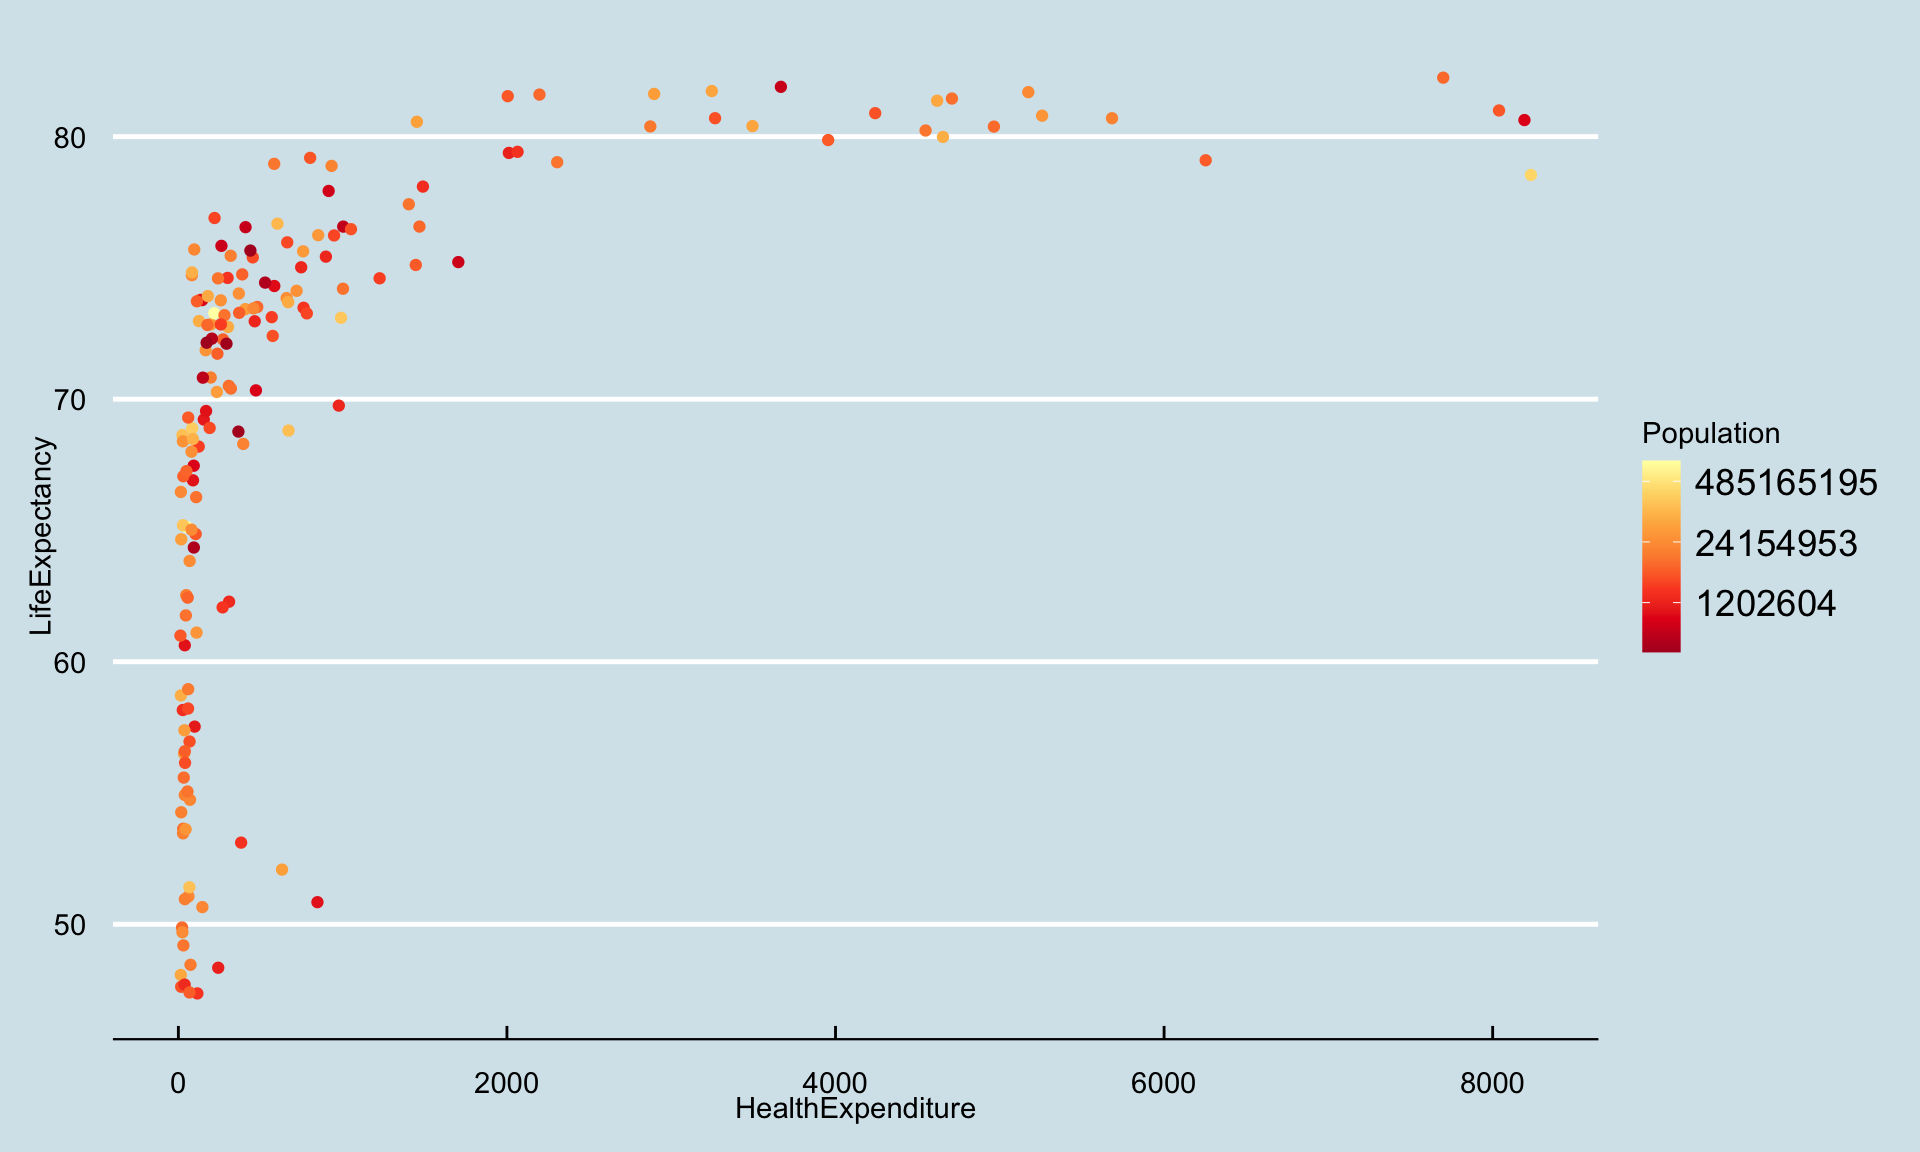
\includegraphics[width=\textwidth]{bookdown-demo_files/figure-latex/unnamed-chunk-64-2}

\hypertarget{arranging-plots-faceting}{%
\subsection{Arranging plots (faceting)}\label{arranging-plots-faceting}}

The function \texttt{facet\_grid(rvar\textasciitilde{}cvar)} creates separate plots based on the values \texttt{rvar} (rows) and \texttt{cvar} (columns) takes. The function \texttt{facet\_wrap(\textasciitilde{}var1+var2)} arranges the plots in several rows and columns without rigidly associating one variable with rows and one with columns. Continuous variables need to be discretised (for example using \texttt{cut}) before they can be used for defining facets.

\begin{Shaded}
\begin{Highlighting}[]
\FunctionTok{ggplot}\NormalTok{(}\AttributeTok{data=}\NormalTok{health) }\SpecialCharTok{+} 
    \FunctionTok{aes}\NormalTok{(}\AttributeTok{x=}\NormalTok{HealthExpenditure,  }\AttributeTok{y=}\NormalTok{LifeExpectancy, }\AttributeTok{colour=}\NormalTok{Region) }\SpecialCharTok{+}
    \FunctionTok{geom\_point}\NormalTok{(}\FunctionTok{aes}\NormalTok{(}\AttributeTok{size=}\NormalTok{Population)) }\SpecialCharTok{+}
    \FunctionTok{geom\_smooth}\NormalTok{(}\AttributeTok{method=}\StringTok{"lm"}\NormalTok{)  }\SpecialCharTok{+}
    \FunctionTok{scale\_x\_log10}\NormalTok{() }\SpecialCharTok{+}
    \FunctionTok{facet\_wrap}\NormalTok{(}\SpecialCharTok{\textasciitilde{}}\NormalTok{Region)}
\end{Highlighting}
\end{Shaded}

\begin{verbatim}
## `geom_smooth()` using formula 'y ~ x'
\end{verbatim}

\begin{verbatim}
## Warning in qt((1 - level)/2, df): NaNs produced
\end{verbatim}

\begin{verbatim}
## Warning in max(ids, na.rm = TRUE): no non-missing arguments to max; returning
## -Inf
\end{verbatim}

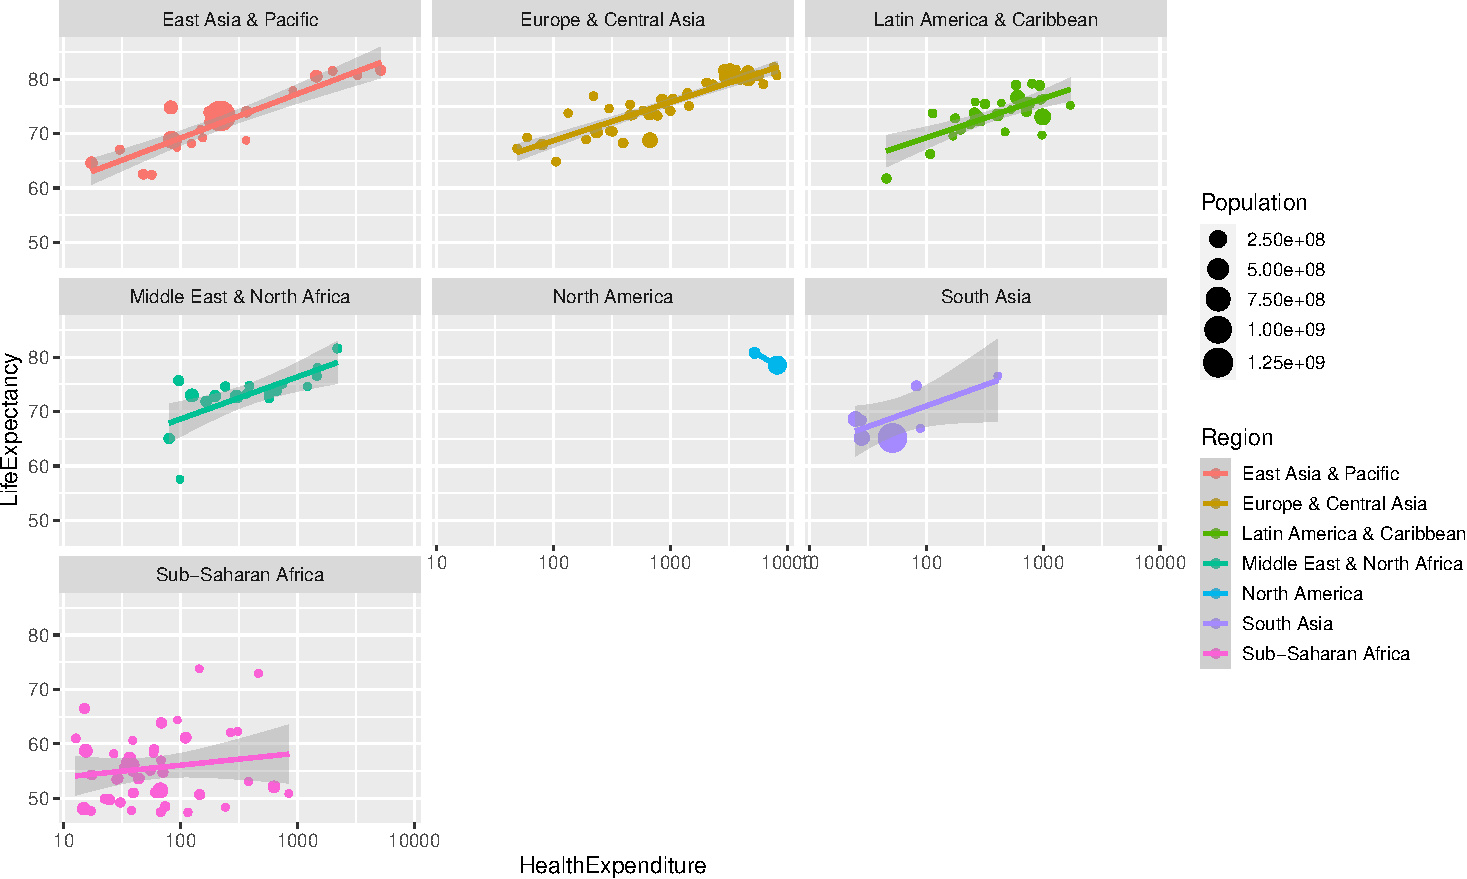
\includegraphics[width=\textwidth]{bookdown-demo_files/figure-latex/unnamed-chunk-65-1}

Arranging plots in more general ways (like in \texttt{par(mfrow=c(...))} or \texttt{layout}) is not directly possible with \texttt{ggplot2}. The package \href{https://cran.r-project.org/web/packages/gridExtra}{gridExtra} however provides a function \texttt{grid.arrange}, which allows for arranging \texttt{ggplot2} plots side by side.

\hypertarget{handling-date-time-data-with-lubridate}{%
\chapter{\texorpdfstring{Handling date-time data with \texttt{lubridate}}{Handling date-time data with lubridate}}\label{handling-date-time-data-with-lubridate}}

Date-time data can be complex to handle in R. Classic R commands for date-times are generally unintuitive and vary depending on the date-time object being used. the \texttt{lubridate} package makes it easier to handle date-times in R and handle many tasks classic R functions cannot handle.

We will cover some useful commands within the package but do consult the \texttt{lubridate} cheat sheet below for a series of useful commands.

\href{\%22https://rawgit.com/rstudio/cheatsheets/main/lubridate.pdf\%22}{Lubridate cheat sheet}

\hypertarget{creating-datetimes}{%
\section{Creating date/times}\label{creating-datetimes}}

There are three types of date/time data that refer to an instant in time:

\begin{itemize}
\tightlist
\item
  A \emph{date}. Tibbles print this as \texttt{\textless{}date\textgreater{}}
\item
  A \emph{time} within a day. Tibbles print this as \texttt{\textless{}time\textgreater{}}
\item
  A \emph{date-time} is a date plus a time: it uniquely identifies an instant in time. Tibbles print this as \texttt{\textless{}dttm\textgreater{}}.
\end{itemize}

You should always use the simplest possible data type for what you need.

There are three ways you are likely to create a date/time:

\begin{itemize}
\tightlist
\item
  From a string
\item
  From date/time components
\item
  From an existing date/time object
\end{itemize}

These can be created as follows.

\hypertarget{from-strings}{%
\subsection{From strings}\label{from-strings}}

We can convert a string to a date/time object using functions within \texttt{lubridate}. These functions automatically work out the format once you specify the order of the component. To use them, identify the order in which year, month and day appear in your dates, then arrange ``y'', ``m'', and ``d'' in the same order. This gives you the name of the function you need to call. For example:

\begin{Shaded}
\begin{Highlighting}[]
\FunctionTok{ymd}\NormalTok{(}\StringTok{"2022{-}08{-}02"}\NormalTok{)}
\end{Highlighting}
\end{Shaded}

\begin{verbatim}
## [1] "2022-08-02"
\end{verbatim}

\begin{Shaded}
\begin{Highlighting}[]
\FunctionTok{mdy}\NormalTok{(}\StringTok{"August 2nd, 2022"}\NormalTok{)}
\end{Highlighting}
\end{Shaded}

\begin{verbatim}
## [1] "2022-08-02"
\end{verbatim}

\begin{Shaded}
\begin{Highlighting}[]
\FunctionTok{dmy}\NormalTok{(}\StringTok{"02{-}Aug{-}2022"}\NormalTok{)}
\end{Highlighting}
\end{Shaded}

\begin{verbatim}
## [1] "2022-08-02"
\end{verbatim}

These functions also take unquoted numbers. This is the most concise way to create a single date/time object.

\begin{Shaded}
\begin{Highlighting}[]
\FunctionTok{ymd}\NormalTok{(}\DecValTok{20220802}\NormalTok{)}
\end{Highlighting}
\end{Shaded}

\begin{verbatim}
## [1] "2022-08-02"
\end{verbatim}

To create a date-time, add an underscore to the previous functions and one or more of ``h'', ``m'' and ``s'' to the name of the function

\begin{Shaded}
\begin{Highlighting}[]
\FunctionTok{ymd\_hms}\NormalTok{(}\StringTok{"2022{-}08{-}02 13:05:02"}\NormalTok{)}
\end{Highlighting}
\end{Shaded}

\begin{verbatim}
## [1] "2022-08-02 13:05:02 UTC"
\end{verbatim}

\begin{Shaded}
\begin{Highlighting}[]
\FunctionTok{mdy\_hm}\NormalTok{(}\StringTok{"08/02/2022 13:05"}\NormalTok{)}
\end{Highlighting}
\end{Shaded}

\begin{verbatim}
## [1] "2022-08-02 13:05:00 UTC"
\end{verbatim}

You can also force the creation of a date-time from a date by supplying a timezone

\begin{Shaded}
\begin{Highlighting}[]
\FunctionTok{ymd}\NormalTok{(}\DecValTok{20220802}\NormalTok{,}\AttributeTok{tz=}\StringTok{"UTC"}\NormalTok{)}
\end{Highlighting}
\end{Shaded}

\begin{verbatim}
## [1] "2022-08-02 UTC"
\end{verbatim}

\hypertarget{from-individual-components}{%
\subsection{From individual components}\label{from-individual-components}}

Instead of a string, you sometimes may have individual components of the date-time spread across multiple columns. Looking at data provided within the \texttt{nycflights13} library, we see

\begin{Shaded}
\begin{Highlighting}[]
\FunctionTok{library}\NormalTok{(nycflights13)}
\FunctionTok{library}\NormalTok{(tidyverse)}

\NormalTok{flights }\SpecialCharTok{\%\textgreater{}\%}
  \FunctionTok{select}\NormalTok{(year,month,day,hour,minute)}
\end{Highlighting}
\end{Shaded}

\begin{verbatim}
## # A tibble: 336,776 x 5
##     year month   day  hour minute
##    <int> <int> <int> <dbl>  <dbl>
##  1  2013     1     1     5     15
##  2  2013     1     1     5     29
##  3  2013     1     1     5     40
##  4  2013     1     1     5     45
##  5  2013     1     1     6      0
##  6  2013     1     1     5     58
##  7  2013     1     1     6      0
##  8  2013     1     1     6      0
##  9  2013     1     1     6      0
## 10  2013     1     1     6      0
## # ... with 336,766 more rows
\end{verbatim}

To create a date/time for this data, we can use \texttt{make\_date()} for dates, or \texttt{make\_datetime()} for date-times:

\begin{Shaded}
\begin{Highlighting}[]
\NormalTok{flights }\OtherTok{\textless{}{-}}\NormalTok{ flights }\SpecialCharTok{\%\textgreater{}\%}
  \FunctionTok{select}\NormalTok{(year,month,day,hour,minute) }\SpecialCharTok{\%\textgreater{}\%}
  \FunctionTok{mutate}\NormalTok{(}\AttributeTok{departure\_time=}\FunctionTok{make\_datetime}\NormalTok{(year,month,day,hour,minute))}
\end{Highlighting}
\end{Shaded}

\hypertarget{from-existing-types}{%
\subsection{From existing types}\label{from-existing-types}}

You may wish to switch between a date-time and a date. This can be done using \texttt{as\_datetime()} and \texttt{as\_date()}

\begin{Shaded}
\begin{Highlighting}[]
\FunctionTok{as\_datetime}\NormalTok{(}\FunctionTok{today}\NormalTok{())}
\end{Highlighting}
\end{Shaded}

\begin{verbatim}
## [1] "2022-08-15 UTC"
\end{verbatim}

\begin{Shaded}
\begin{Highlighting}[]
\FunctionTok{as\_date}\NormalTok{(}\FunctionTok{now}\NormalTok{())}
\end{Highlighting}
\end{Shaded}

\begin{verbatim}
## [1] "2022-08-15"
\end{verbatim}

\hypertarget{date-time-components}{%
\section{Date-time Components}\label{date-time-components}}

Here, we will look at functions which can let us access certain components of a date-time object.

You can obtain certain parts of a date with functions like \texttt{year()}, \texttt{month()}, \texttt{mday()} (day of month), \texttt{yday()} (day of year), \texttt{hour()}, \texttt{minute()} and \texttt{second()}.

\begin{Shaded}
\begin{Highlighting}[]
\NormalTok{date\_time }\OtherTok{\textless{}{-}} \FunctionTok{ymd\_hms}\NormalTok{(}\StringTok{"2021{-}12{-}25,09:10:25"}\NormalTok{)}

\FunctionTok{year}\NormalTok{(date\_time)}
\end{Highlighting}
\end{Shaded}

\begin{verbatim}
## [1] 2021
\end{verbatim}

\begin{Shaded}
\begin{Highlighting}[]
\FunctionTok{month}\NormalTok{(date\_time)}
\end{Highlighting}
\end{Shaded}

\begin{verbatim}
## [1] 12
\end{verbatim}

\begin{Shaded}
\begin{Highlighting}[]
\FunctionTok{mday}\NormalTok{(date\_time)}
\end{Highlighting}
\end{Shaded}

\begin{verbatim}
## [1] 25
\end{verbatim}

\begin{Shaded}
\begin{Highlighting}[]
\FunctionTok{yday}\NormalTok{(date\_time)}
\end{Highlighting}
\end{Shaded}

\begin{verbatim}
## [1] 359
\end{verbatim}

For \texttt{month()} and \texttt{wday()}, you can set \texttt{label=TRUE} to return the abbreviated name of the month or day of the week. Set \texttt{abbr=FALSE} to return the full name.

\begin{Shaded}
\begin{Highlighting}[]
\FunctionTok{month}\NormalTok{(date\_time,}\AttributeTok{label=}\ConstantTok{TRUE}\NormalTok{)}
\end{Highlighting}
\end{Shaded}

\begin{verbatim}
## [1] Dec
## 12 Levels: Jan < Feb < Mar < Apr < May < Jun < Jul < Aug < Sep < ... < Dec
\end{verbatim}

\begin{Shaded}
\begin{Highlighting}[]
\FunctionTok{wday}\NormalTok{(date\_time,}\AttributeTok{label=}\ConstantTok{TRUE}\NormalTok{,}\AttributeTok{abbr=}\ConstantTok{FALSE}\NormalTok{)}
\end{Highlighting}
\end{Shaded}

\begin{verbatim}
## [1] Saturday
## 7 Levels: Sunday < Monday < Tuesday < Wednesday < Thursday < ... < Saturday
\end{verbatim}

We can use \texttt{wday()} to see that more flights depart during the week than on the weekend

\begin{Shaded}
\begin{Highlighting}[]
\NormalTok{flights }\SpecialCharTok{\%\textgreater{}\%} 
  \FunctionTok{mutate}\NormalTok{(}\AttributeTok{wday =} \FunctionTok{wday}\NormalTok{(departure\_time, }\AttributeTok{label =} \ConstantTok{TRUE}\NormalTok{)) }\SpecialCharTok{\%\textgreater{}\%} 
  \FunctionTok{ggplot}\NormalTok{(}\FunctionTok{aes}\NormalTok{(}\AttributeTok{x =}\NormalTok{ wday)) }\SpecialCharTok{+}
    \FunctionTok{geom\_bar}\NormalTok{()}
\end{Highlighting}
\end{Shaded}

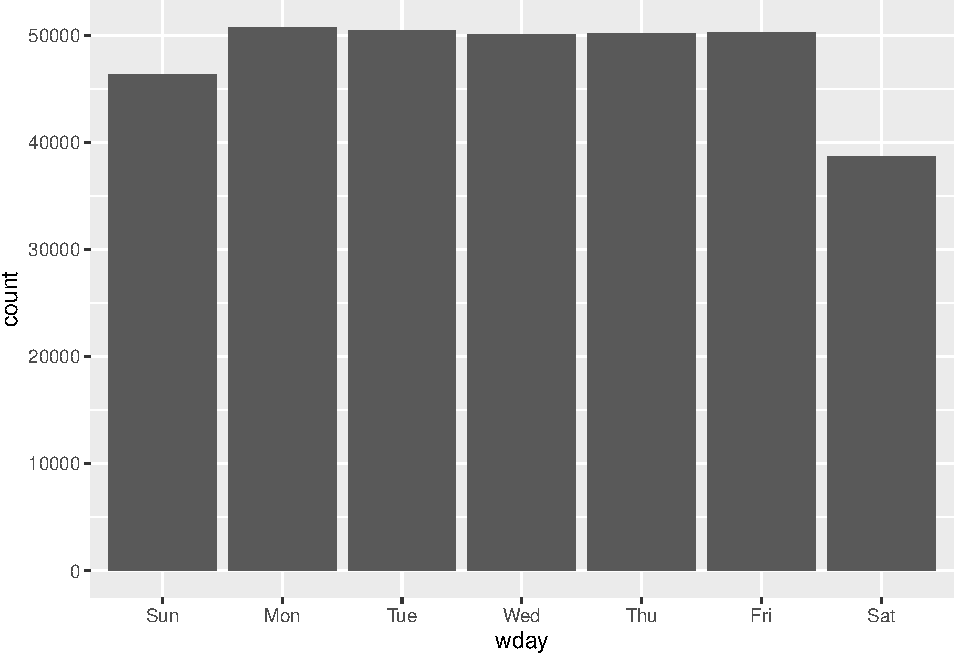
\includegraphics{bookdown-demo_files/figure-latex/unnamed-chunk-76-1.pdf}

\hypertarget{time-spans}{%
\subsection{Time Spans}\label{time-spans}}

Now we will look at how arithmetic with dates works, including subtraction, addition and division. We will explore the following three classes:

\begin{itemize}
\tightlist
\item
  \emph{durations}, which represent an exact number of seconds
\item
  \emph{periods}, which represent units like weeks and months
\item
  \emph{intervals}, which represent a start and end point
\end{itemize}

\hypertarget{durations}{%
\subsection{Durations}\label{durations}}

We can find out the duration (given in seconds) using the \texttt{as.duration()} function as shown below

\begin{Shaded}
\begin{Highlighting}[]
\CommentTok{\# How old is Craig?}
\NormalTok{c\_age }\OtherTok{\textless{}{-}} \FunctionTok{today}\NormalTok{() }\SpecialCharTok{{-}} \FunctionTok{ymd}\NormalTok{(}\DecValTok{19910502}\NormalTok{)}
\FunctionTok{as.duration}\NormalTok{(c\_age)}
\end{Highlighting}
\end{Shaded}

\begin{verbatim}
## [1] "987379200s (~31.29 years)"
\end{verbatim}

Durations also come with some useful additional functions shown below

\begin{Shaded}
\begin{Highlighting}[]
\FunctionTok{dseconds}\NormalTok{(}\DecValTok{10}\NormalTok{)}
\end{Highlighting}
\end{Shaded}

\begin{verbatim}
## [1] "10s"
\end{verbatim}

\begin{Shaded}
\begin{Highlighting}[]
\FunctionTok{dminutes}\NormalTok{(}\DecValTok{60}\NormalTok{)}
\end{Highlighting}
\end{Shaded}

\begin{verbatim}
## [1] "3600s (~1 hours)"
\end{verbatim}

\begin{Shaded}
\begin{Highlighting}[]
\FunctionTok{dhours}\NormalTok{(}\DecValTok{30}\NormalTok{)}
\end{Highlighting}
\end{Shaded}

\begin{verbatim}
## [1] "108000s (~1.25 days)"
\end{verbatim}

\begin{Shaded}
\begin{Highlighting}[]
\FunctionTok{ddays}\NormalTok{(}\FunctionTok{c}\NormalTok{(}\DecValTok{4}\NormalTok{,}\DecValTok{15}\NormalTok{))}
\end{Highlighting}
\end{Shaded}

\begin{verbatim}
## [1] "345600s (~4 days)"      "1296000s (~2.14 weeks)"
\end{verbatim}

\begin{Shaded}
\begin{Highlighting}[]
\FunctionTok{dweeks}\NormalTok{(}\DecValTok{1}\SpecialCharTok{:}\DecValTok{4}\NormalTok{)}
\end{Highlighting}
\end{Shaded}

\begin{verbatim}
## [1] "604800s (~1 weeks)"  "1209600s (~2 weeks)" "1814400s (~3 weeks)"
## [4] "2419200s (~4 weeks)"
\end{verbatim}

\begin{Shaded}
\begin{Highlighting}[]
\FunctionTok{dyears}\NormalTok{(}\DecValTok{2}\NormalTok{)}
\end{Highlighting}
\end{Shaded}

\begin{verbatim}
## [1] "63115200s (~2 years)"
\end{verbatim}

We can also add and multiply durations

\begin{Shaded}
\begin{Highlighting}[]
\DecValTok{3}\SpecialCharTok{*}\FunctionTok{dmonths}\NormalTok{(}\DecValTok{5}\NormalTok{)}
\end{Highlighting}
\end{Shaded}

\begin{verbatim}
## [1] "39447000s (~1.25 years)"
\end{verbatim}

\begin{Shaded}
\begin{Highlighting}[]
\FunctionTok{dyears}\NormalTok{(}\DecValTok{3}\NormalTok{) }\SpecialCharTok{+} \FunctionTok{dweeks}\NormalTok{(}\DecValTok{14}\NormalTok{) }\SpecialCharTok{+}\FunctionTok{dhours}\NormalTok{(}\DecValTok{6}\NormalTok{)}
\end{Highlighting}
\end{Shaded}

\begin{verbatim}
## [1] "103161600s (~3.27 years)"
\end{verbatim}

\hypertarget{periods}{%
\subsection{Periods}\label{periods}}

Periods are time spans, but don't have a fixed length in seconds, and work more as ``human'' times, like days and weeks.

\begin{Shaded}
\begin{Highlighting}[]
\FunctionTok{today}\NormalTok{() }\SpecialCharTok{+} \FunctionTok{days}\NormalTok{(}\DecValTok{1}\NormalTok{)}
\end{Highlighting}
\end{Shaded}

\begin{verbatim}
## [1] "2022-08-16"
\end{verbatim}

Like durations, periods can be constructed using well named constructor functions.

\begin{Shaded}
\begin{Highlighting}[]
\FunctionTok{seconds}\NormalTok{(}\DecValTok{15}\NormalTok{)}
\end{Highlighting}
\end{Shaded}

\begin{verbatim}
## [1] "15S"
\end{verbatim}

\begin{Shaded}
\begin{Highlighting}[]
\FunctionTok{minutes}\NormalTok{(}\DecValTok{10}\NormalTok{)}
\end{Highlighting}
\end{Shaded}

\begin{verbatim}
## [1] "10M 0S"
\end{verbatim}

\begin{Shaded}
\begin{Highlighting}[]
\FunctionTok{hours}\NormalTok{(}\DecValTok{30}\NormalTok{)}
\end{Highlighting}
\end{Shaded}

\begin{verbatim}
## [1] "30H 0M 0S"
\end{verbatim}

\begin{Shaded}
\begin{Highlighting}[]
\FunctionTok{days}\NormalTok{(}\FunctionTok{c}\NormalTok{(}\DecValTok{2}\NormalTok{,}\DecValTok{5}\NormalTok{))}
\end{Highlighting}
\end{Shaded}

\begin{verbatim}
## [1] "2d 0H 0M 0S" "5d 0H 0M 0S"
\end{verbatim}

\begin{Shaded}
\begin{Highlighting}[]
\FunctionTok{months}\NormalTok{(}\DecValTok{2}\SpecialCharTok{:}\DecValTok{5}\NormalTok{)}
\end{Highlighting}
\end{Shaded}

\begin{verbatim}
## [1] "2m 0d 0H 0M 0S" "3m 0d 0H 0M 0S" "4m 0d 0H 0M 0S" "5m 0d 0H 0M 0S"
\end{verbatim}

\begin{Shaded}
\begin{Highlighting}[]
\FunctionTok{weeks}\NormalTok{(}\DecValTok{3}\NormalTok{)}
\end{Highlighting}
\end{Shaded}

\begin{verbatim}
## [1] "21d 0H 0M 0S"
\end{verbatim}

\begin{Shaded}
\begin{Highlighting}[]
\FunctionTok{years}\NormalTok{(}\DecValTok{1}\NormalTok{)}
\end{Highlighting}
\end{Shaded}

\begin{verbatim}
## [1] "1y 0m 0d 0H 0M 0S"
\end{verbatim}

Like durations, we can add and multiply periods

\begin{Shaded}
\begin{Highlighting}[]
\DecValTok{3}\SpecialCharTok{*}\NormalTok{(}\FunctionTok{months}\NormalTok{(}\DecValTok{4}\NormalTok{) }\SpecialCharTok{+} \FunctionTok{days}\NormalTok{(}\DecValTok{12}\NormalTok{))}
\end{Highlighting}
\end{Shaded}

\begin{verbatim}
## [1] "12m 36d 0H 0M 0S"
\end{verbatim}

\begin{Shaded}
\begin{Highlighting}[]
\FunctionTok{days}\NormalTok{(}\DecValTok{25}\NormalTok{) }\SpecialCharTok{+} \FunctionTok{hours}\NormalTok{(}\DecValTok{16}\NormalTok{) }\SpecialCharTok{+} \FunctionTok{minutes}\NormalTok{(}\DecValTok{12}\NormalTok{)}
\end{Highlighting}
\end{Shaded}

\begin{verbatim}
## [1] "25d 16H 12M 0S"
\end{verbatim}

\hypertarget{intervals}{%
\subsection{Intervals}\label{intervals}}

An interval is a duration with a starting point, this makes it precise so you can determine exactly how long it is:

\begin{Shaded}
\begin{Highlighting}[]
\NormalTok{next\_year }\OtherTok{\textless{}{-}} \FunctionTok{today}\NormalTok{() }\SpecialCharTok{+} \FunctionTok{years}\NormalTok{(}\DecValTok{1}\NormalTok{)}
\NormalTok{(}\FunctionTok{today}\NormalTok{() }\SpecialCharTok{\%{-}{-}\%}\NormalTok{ next\_year)}\SpecialCharTok{/}\FunctionTok{ddays}\NormalTok{(}\DecValTok{1}\NormalTok{)}
\end{Highlighting}
\end{Shaded}

\begin{verbatim}
## [1] 365
\end{verbatim}

To find out how many periods fall into an interval, you need to use integer division \texttt{\%/\%}

\hypertarget{producing-maps-for-plotting}{%
\chapter{Producing maps for plotting}\label{producing-maps-for-plotting}}

\hypertarget{producing-maps-using-ggmap}{%
\section{Producing maps using ggmap}\label{producing-maps-using-ggmap}}

The R package \texttt{ggmap} can download maps from Google maps (or OpenStreetMap) which can then be used as a background layer in a \texttt{ggplot2} plot.

The function \texttt{get\_map(location,\ zoom)} downloads a map. \texttt{location} can be a pair of longitude and latitude, a character string describing the location, or a bounding box. \texttt{zoom} controls the zoom level (from 3 (continent) to 21 (highest resolution)). The optional argument \texttt{maptype} can be used to select the type of map downloaded (for example \texttt{"roadmap"}, \texttt{"hybrid"} or \texttt{"satellite"} when using Google maps)

Note that access to the Google API (for Google map tiles and for geolocation (translation of location description to GPS coordinates) requires a Google API key. When using a bounding box and \texttt{"stamen"} as \texttt{source}, no API key is required.

\begin{Shaded}
\begin{Highlighting}[]
\FunctionTok{library}\NormalTok{(ggmap)}
\NormalTok{boundingbox }\OtherTok{\textless{}{-}} \FunctionTok{c}\NormalTok{(}\AttributeTok{left =} \FloatTok{5.855}\NormalTok{, }\AttributeTok{bottom =} \FloatTok{51.817}\NormalTok{, }\AttributeTok{right =} \FloatTok{5.871}\NormalTok{, }\AttributeTok{top =} \FloatTok{51.826}\NormalTok{)}
\NormalTok{map }\OtherTok{\textless{}{-}} \FunctionTok{get\_map}\NormalTok{(boundingbox, }\AttributeTok{zoom=}\DecValTok{16}\NormalTok{, }\AttributeTok{source=}\StringTok{"stamen"}\NormalTok{)}
\end{Highlighting}
\end{Shaded}

The map can the be plotted using \texttt{ggmap(map)}. Layers can be added to the map using the usual \texttt{ggplot2} commands.

\begin{Shaded}
\begin{Highlighting}[]
\FunctionTok{ggmap}\NormalTok{(map) }\SpecialCharTok{+} 
    \FunctionTok{geom\_label}\NormalTok{(}\AttributeTok{x=}\FloatTok{5.862}\NormalTok{, }\AttributeTok{y=}\FloatTok{51.823}\NormalTok{, }\AttributeTok{label=}\StringTok{"Radboud University"}\NormalTok{) }
\end{Highlighting}
\end{Shaded}

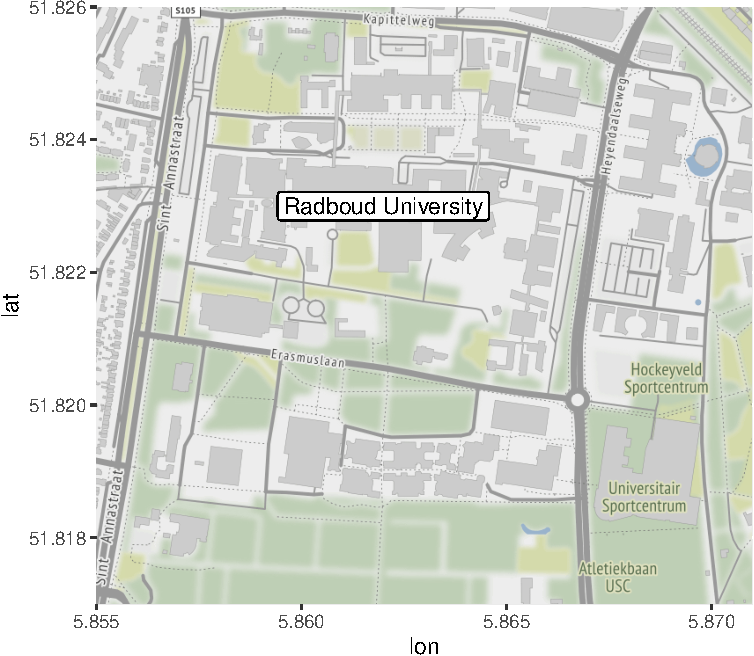
\includegraphics{bookdown-demo_files/figure-latex/unnamed-chunk-85-1.pdf}

\hypertarget{task-8}{%
\subsection{Task}\label{task-8}}

In this task, we will use data from two tibbles, \texttt{stations} and \texttt{trips}. These contain information on the list of bike stations of the Bay Area Bike Share system in the San Francisco Bay Area.

You can download the data using the following command

\begin{Shaded}
\begin{Highlighting}[]
\FunctionTok{load}\NormalTok{(}\FunctionTok{url}\NormalTok{(}\StringTok{"https://github.com/UofGAnalyticsData/R/raw/main/Week\%206/t3.RData"}\NormalTok{))}
\end{Highlighting}
\end{Shaded}

It has the following columns.

\begin{longtable}[]{@{}ll@{}}
\toprule()
Column name & Description \\
\midrule()
\endhead
\texttt{station\_id} & Numeric identifier of the station \\
\texttt{name} & Name of the station \\
\texttt{lat} & Latitude of the station \\
\texttt{long} & Longitude of the station \\
\texttt{dockcount} & Number of docks at the station \\
\texttt{city} & City in which the station is located \\
\bottomrule()
\end{longtable}

The tibble \texttt{trips} contains all trips made during August 2015. It has the following columns.

\begin{longtable}[]{@{}
  >{\raggedright\arraybackslash}p{(\columnwidth - 2\tabcolsep) * \real{0.2889}}
  >{\raggedright\arraybackslash}p{(\columnwidth - 2\tabcolsep) * \real{0.7111}}@{}}
\toprule()
\begin{minipage}[b]{\linewidth}\raggedright
Column name
\end{minipage} & \begin{minipage}[b]{\linewidth}\raggedright
Description
\end{minipage} \\
\midrule()
\endhead
\texttt{trip\_id} & Numeric identifier of the trip \\
\texttt{trip\_duration} & Duration of the trip in seconds \\
\texttt{day} & Day of the month the trip was started \\
\texttt{hour} & Decimal hour when the strip was started \\
\texttt{start\_station\_id} & Numeric identifier of the station where the trip started \\
\texttt{end\_station\_id} & Numeric identifier of the station where the trip ended \\
\texttt{bike\_id} & Numeric identifier of the bike used \\
\texttt{end\_date} & Date and time the trip ended \\
\texttt{subscriber\_type} & User type (``Subscriber'' or ``Customer'') \\
\bottomrule()
\end{longtable}

\begin{enumerate}
\def\labelenumi{\alph{enumi})}
\tightlist
\item
  Plot the locations of each of the bike stations. You can use the following bounding box below for your map
\end{enumerate}

\begin{Shaded}
\begin{Highlighting}[]
\NormalTok{boundingbox }\OtherTok{\textless{}{-}} \FunctionTok{c}\NormalTok{(}\AttributeTok{left =} \SpecialCharTok{{-}}\FloatTok{122.5}\NormalTok{, }\AttributeTok{bottom =} \FloatTok{37.25}\NormalTok{, }\AttributeTok{right =} \SpecialCharTok{{-}}\FloatTok{121.75}\NormalTok{, }\AttributeTok{top =} \DecValTok{38}\NormalTok{)}
\end{Highlighting}
\end{Shaded}

\begin{enumerate}
\def\labelenumi{\alph{enumi})}
\setcounter{enumi}{1}
\tightlist
\item
  (Harder) For trips within the city of San Francisco, use the code below to create an origin-destination matrix. The \((i,j)\)th entry contains the number of trips from station \(i\) to station \(j\).
\end{enumerate}

Create a plot representing the number of trips between the stations. Use the line thickness or transparency to indicate the number of trips. You can use the following bounding box below for your map

\begin{Shaded}
\begin{Highlighting}[]
\FunctionTok{library}\NormalTok{(tidyverse)}

\NormalTok{sf\_stations }\OtherTok{\textless{}{-}}\NormalTok{ stations }\SpecialCharTok{\%\textgreater{}\%}
    \FunctionTok{filter}\NormalTok{(city}\SpecialCharTok{==}\StringTok{"San Francisco"}\NormalTok{) }

\NormalTok{od }\OtherTok{\textless{}{-}}\NormalTok{ trips }\SpecialCharTok{\%\textgreater{}\%}
         \FunctionTok{filter}\NormalTok{(start\_station\_id}\SpecialCharTok{\%in\%}\NormalTok{sf\_stations}\SpecialCharTok{$}\NormalTok{station\_id,}
\NormalTok{                end\_station\_id}\SpecialCharTok{\%in\%}\NormalTok{sf\_stations}\SpecialCharTok{$}\NormalTok{station\_id) }\SpecialCharTok{\%\textgreater{}\%}
         \FunctionTok{group\_by}\NormalTok{(start\_station\_id, end\_station\_id) }\SpecialCharTok{\%\textgreater{}\%}
         \FunctionTok{summarise}\NormalTok{(}\AttributeTok{ntrips=}\FunctionTok{n}\NormalTok{()) }
\end{Highlighting}
\end{Shaded}

\begin{verbatim}
## `summarise()` has grouped output by 'start_station_id'. You can override using
## the `.groups` argument.
\end{verbatim}

\begin{Shaded}
\begin{Highlighting}[]
\NormalTok{odm }\OtherTok{\textless{}{-}}\NormalTok{ od }\SpecialCharTok{\%\textgreater{}\%}
         \FunctionTok{spread}\NormalTok{(end\_station\_id, ntrips, }\AttributeTok{fill=}\DecValTok{0}\NormalTok{) }

\NormalTok{odm }\OtherTok{\textless{}{-}} \FunctionTok{as.matrix}\NormalTok{(od[,}\SpecialCharTok{{-}}\DecValTok{1}\NormalTok{])}
\FunctionTok{rownames}\NormalTok{(odm) }\OtherTok{\textless{}{-}}\NormalTok{ od}\SpecialCharTok{$}\NormalTok{start\_station\_id}

\NormalTok{od2 }\OtherTok{\textless{}{-}}\NormalTok{ od }\SpecialCharTok{\%\textgreater{}\%} 
    \FunctionTok{full\_join}\NormalTok{(od, }\AttributeTok{by=}\FunctionTok{c}\NormalTok{(}\StringTok{"start\_station\_id"}\OtherTok{=}\StringTok{"end\_station\_id"}\NormalTok{, }\StringTok{"end\_station\_id"}\OtherTok{=}
\StringTok{"start\_station\_id"}\NormalTok{)) }\SpecialCharTok{\%\textgreater{}\%}
    \FunctionTok{replace\_na}\NormalTok{(}\FunctionTok{list}\NormalTok{(}\AttributeTok{ntrips.x=}\DecValTok{0}\NormalTok{, }\AttributeTok{ntrips.y=}\DecValTok{0}\NormalTok{)) }\SpecialCharTok{\%\textgreater{}\%}
    \FunctionTok{mutate}\NormalTok{(}\AttributeTok{ntrips=}\NormalTok{ntrips.x}\SpecialCharTok{+}\NormalTok{ntrips.y) }\SpecialCharTok{\%\textgreater{}\%}
    \FunctionTok{select}\NormalTok{(}\SpecialCharTok{{-}}\NormalTok{ntrips.x, }\SpecialCharTok{{-}}\NormalTok{ntrips.y) }\SpecialCharTok{\%\textgreater{}\%}
    \FunctionTok{filter}\NormalTok{(start\_station\_id}\SpecialCharTok{\textless{}}\NormalTok{end\_station\_id)}

\NormalTok{odall }\OtherTok{\textless{}{-}} 
\NormalTok{    od2 }\SpecialCharTok{\%\textgreater{}\%} 
    \FunctionTok{inner\_join}\NormalTok{(sf\_stations, }\AttributeTok{by=}\FunctionTok{c}\NormalTok{(}\StringTok{"start\_station\_id"}\OtherTok{=}\StringTok{"station\_id"}\NormalTok{)) }\SpecialCharTok{\%\textgreater{}\%}
    \FunctionTok{inner\_join}\NormalTok{(sf\_stations, }\AttributeTok{by=}\FunctionTok{c}\NormalTok{(}\StringTok{"end\_station\_id"}\OtherTok{=}\StringTok{"station\_id"}\NormalTok{), }\AttributeTok{suffix=}\FunctionTok{c}\NormalTok{(}\StringTok{""}\NormalTok{,}\StringTok{"\_end"}\NormalTok{))}


\NormalTok{boundingbox }\OtherTok{\textless{}{-}} \FunctionTok{c}\NormalTok{(}\AttributeTok{left =} \SpecialCharTok{{-}}\FloatTok{122.43}\NormalTok{, }\AttributeTok{bottom =} \FloatTok{37.76}\NormalTok{, }\AttributeTok{right =} \SpecialCharTok{{-}}\FloatTok{122.38}\NormalTok{, }\AttributeTok{top =} \FloatTok{37.81}\NormalTok{)}
\end{Highlighting}
\end{Shaded}

\hypertarget{answer-7}{%
\subsection{Answer}\label{answer-7}}

For part (a) we can use the following code.

\begin{Shaded}
\begin{Highlighting}[]
\NormalTok{boundingbox }\OtherTok{\textless{}{-}} \FunctionTok{c}\NormalTok{(}\AttributeTok{left =} \SpecialCharTok{{-}}\FloatTok{122.5}\NormalTok{, }\AttributeTok{bottom =} \FloatTok{37.25}\NormalTok{, }\AttributeTok{right =} \SpecialCharTok{{-}}\FloatTok{121.75}\NormalTok{, }\AttributeTok{top =} \DecValTok{38}\NormalTok{)}

\NormalTok{map }\OtherTok{\textless{}{-}} \FunctionTok{get\_map}\NormalTok{(boundingbox, }\AttributeTok{zoom=}\DecValTok{9}\NormalTok{, }\AttributeTok{source=}\StringTok{"stamen"}\NormalTok{)}

\FunctionTok{ggmap}\NormalTok{(map) }\SpecialCharTok{+} 
    \FunctionTok{geom\_point}\NormalTok{(}\AttributeTok{data=}\NormalTok{stations, }\FunctionTok{aes}\NormalTok{(}\AttributeTok{x=}\NormalTok{long, }\AttributeTok{y=}\NormalTok{lat,  }\AttributeTok{colour=}\NormalTok{city)) }\SpecialCharTok{+}
    \FunctionTok{xlab}\NormalTok{(}\StringTok{"Longitude"}\NormalTok{) }\SpecialCharTok{+} \FunctionTok{ylab}\NormalTok{(}\StringTok{"Latitude"}\NormalTok{) }\SpecialCharTok{+} 
    \FunctionTok{ggtitle}\NormalTok{(}\StringTok{"Bicycle stations in the San Francisco Bay Area"}\NormalTok{)}
\end{Highlighting}
\end{Shaded}

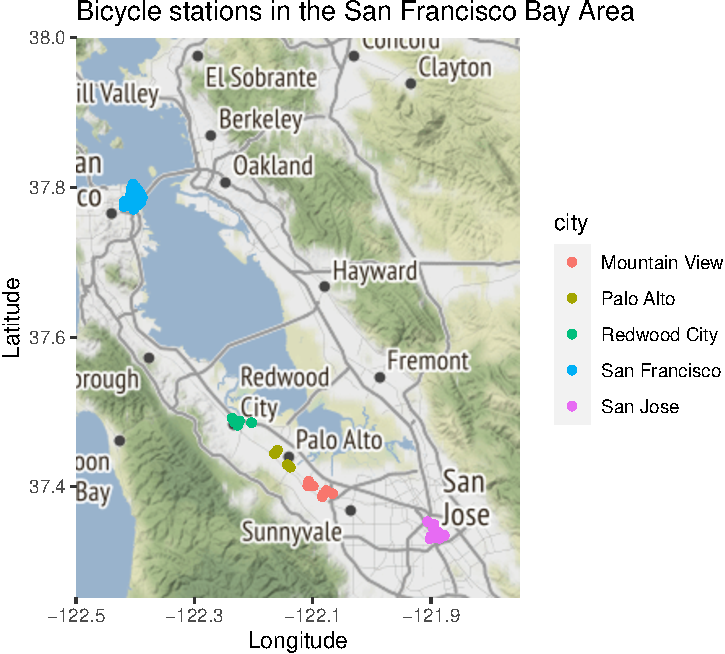
\includegraphics{bookdown-demo_files/figure-latex/unnamed-chunk-89-1.pdf}

For part (b) we can use the following code.

\begin{Shaded}
\begin{Highlighting}[]
\FunctionTok{library}\NormalTok{(magrittr)}
\NormalTok{boundingbox }\OtherTok{\textless{}{-}} \FunctionTok{c}\NormalTok{(}\AttributeTok{left =} \SpecialCharTok{{-}}\FloatTok{122.43}\NormalTok{, }\AttributeTok{bottom =} \FloatTok{37.76}\NormalTok{, }\AttributeTok{right =} \SpecialCharTok{{-}}\FloatTok{122.38}\NormalTok{, }\AttributeTok{top =} \FloatTok{37.81}\NormalTok{)}
\NormalTok{map }\OtherTok{\textless{}{-}} \FunctionTok{get\_map}\NormalTok{(boundingbox, }\AttributeTok{zoom=}\DecValTok{13}\NormalTok{, }\AttributeTok{source=}\StringTok{"stamen"}\NormalTok{)}



\FunctionTok{ggmap}\NormalTok{(map) }\SpecialCharTok{+} 
    \FunctionTok{geom\_point}\NormalTok{(}\AttributeTok{data=}\NormalTok{sf\_stations, }\FunctionTok{aes}\NormalTok{(long, lat, }\AttributeTok{size=}\NormalTok{dockcount), }\AttributeTok{col=}\StringTok{"orange"}\NormalTok{) }\SpecialCharTok{+}
    \FunctionTok{geom\_segment}\NormalTok{(}\AttributeTok{data=}\NormalTok{odall, }\FunctionTok{aes}\NormalTok{(long, lat, }\AttributeTok{xend=}\NormalTok{long\_end, }\AttributeTok{yend=}\NormalTok{lat\_end, }\AttributeTok{alpha=}\NormalTok{ntrips), }\AttributeTok{col=}\StringTok{"orange"}\NormalTok{)}\SpecialCharTok{+}
    \FunctionTok{xlab}\NormalTok{(}\StringTok{"Longitude"}\NormalTok{) }\SpecialCharTok{+} \FunctionTok{ylab}\NormalTok{(}\StringTok{"Latitude"}\NormalTok{) }\SpecialCharTok{+} 
    \FunctionTok{ggtitle}\NormalTok{(}\StringTok{"Bicycle trips in San Francisco"}\NormalTok{)}
\end{Highlighting}
\end{Shaded}

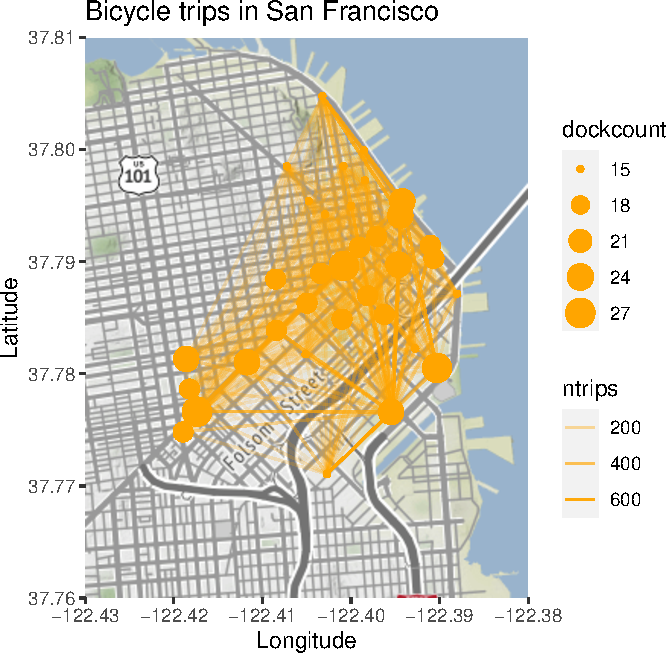
\includegraphics{bookdown-demo_files/figure-latex/unnamed-chunk-90-1.pdf}

\hypertarget{producing-maps-using-leaflet}{%
\subsection{Producing maps using leaflet}\label{producing-maps-using-leaflet}}

Maps plotted using \texttt{ggmap} cannot be panned and zoomed in and out like maps on Google Maps or OpenStreetMap. The package \texttt{leaflet} allows for this. It works somewhat the other way round than \texttt{ggmap}: rather than downloading the map and integrating it into an R plot it overlays the data over the map interface.

The following command puts a marker where Radboud University is located.

\begin{Shaded}
\begin{Highlighting}[]
\FunctionTok{library}\NormalTok{(leaflet)}
\FunctionTok{leaflet}\NormalTok{() }\SpecialCharTok{\%\textgreater{}\%}
   \FunctionTok{addTiles}\NormalTok{(}\AttributeTok{urlTemplate =} \StringTok{"http://\{s\}.tile.openstreetmap.org/\{z\}/\{x\}/\{y\}.png"}\NormalTok{) }\SpecialCharTok{\%\textgreater{}\%} 
   \FunctionTok{addMarkers}\NormalTok{(}\AttributeTok{lng=}\FloatTok{5.862}\NormalTok{, }\AttributeTok{lat=}\FloatTok{51.823}\NormalTok{, }\AttributeTok{popup=}\StringTok{"Radboud University"}\NormalTok{)}
\end{Highlighting}
\end{Shaded}

The argument \texttt{urlTemplate} is only required when opening the file locally.

\begin{figure}
\centering
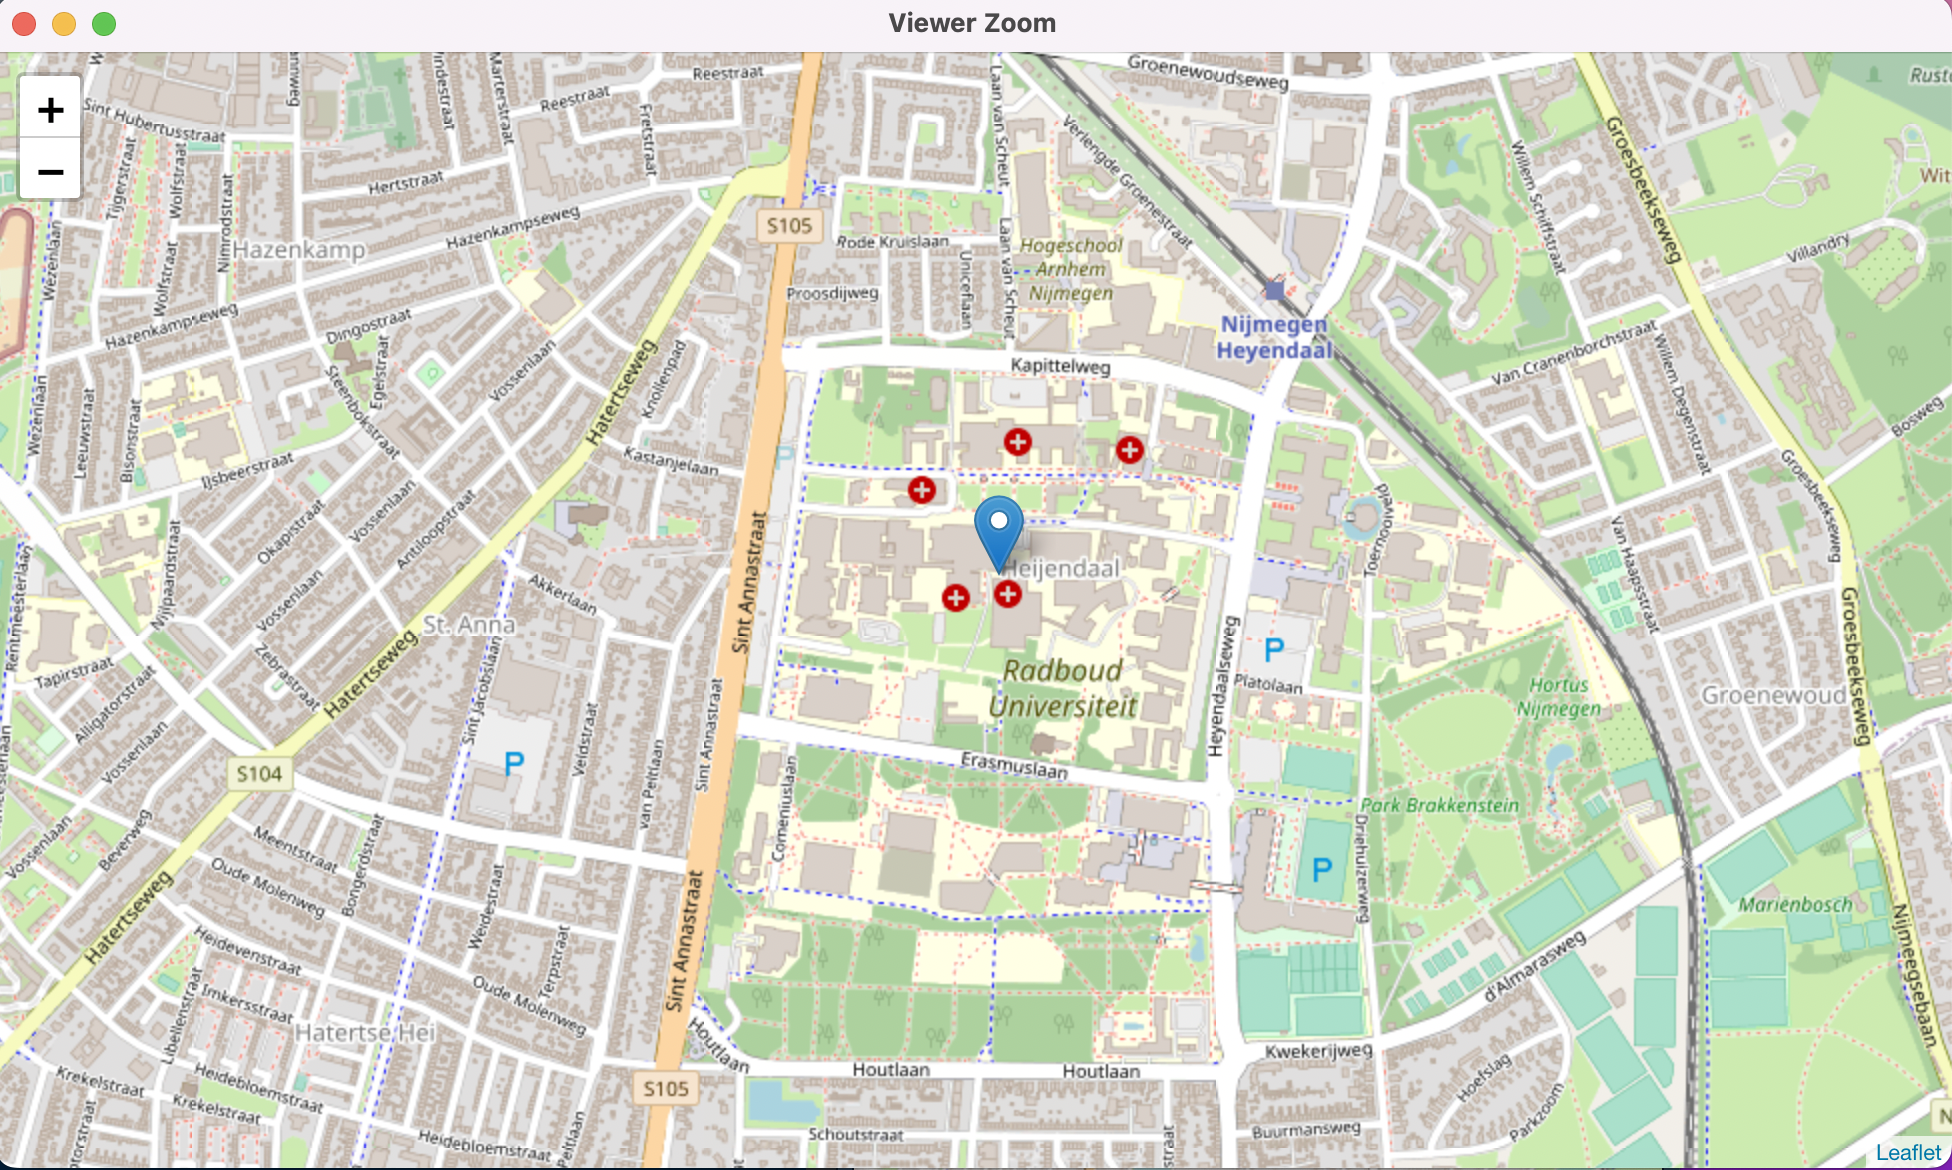
\includegraphics{leaflet1.png}
\caption{Leaflet map showing Radboud University}
\end{figure}

Lines can be added to the map using the function \texttt{addPolylines}.

The data frame \texttt{subway} contains the GPS coordinates of all subway stations in Glasgow. You can produce a map of the Glasgow subway network using the following code. (You should have access to this data frame from the previous download).

\begin{Shaded}
\begin{Highlighting}[]
\NormalTok{subway2 }\OtherTok{\textless{}{-}} \FunctionTok{rbind}\NormalTok{(subway, subway[}\DecValTok{1}\NormalTok{,])     }\CommentTok{\# Make sure line goes back to Hillhead}
\FunctionTok{leaflet}\NormalTok{() }\SpecialCharTok{\%\textgreater{}\%}   
   \FunctionTok{addTiles}\NormalTok{(}\AttributeTok{urlTemplate =} \StringTok{"http://\{s\}.tile.openstreetmap.org/\{z\}/\{x\}/\{y\}.png"}\NormalTok{) }\SpecialCharTok{\%\textgreater{}\%} 
   \FunctionTok{addMarkers}\NormalTok{(}\AttributeTok{lng=}\SpecialCharTok{{-}}\FloatTok{4.2885}\NormalTok{, }\AttributeTok{lat=}\FloatTok{55.8715}\NormalTok{, }\AttributeTok{popup=}\StringTok{"The University of Glasgow"}\NormalTok{) }\SpecialCharTok{\%\textgreater{}\%}
   \FunctionTok{addPolylines}\NormalTok{(subway2}\SpecialCharTok{$}\NormalTok{long, subway2}\SpecialCharTok{$}\NormalTok{lat, }\AttributeTok{color=}\StringTok{"\#ff6200"}\NormalTok{, }\AttributeTok{opacity=}\FloatTok{0.5}\NormalTok{, }\AttributeTok{weight=}\DecValTok{10}\NormalTok{) }\SpecialCharTok{\%\textgreater{}\%} 
   \FunctionTok{addCircleMarkers}\NormalTok{(subway}\SpecialCharTok{$}\NormalTok{long, subway}\SpecialCharTok{$}\NormalTok{lat, }\AttributeTok{popup=}\NormalTok{subway}\SpecialCharTok{$}\NormalTok{station, }\AttributeTok{color=}\StringTok{"\#ff6200"}\NormalTok{, }
                    \AttributeTok{opacity=}\DecValTok{1}\NormalTok{, }\AttributeTok{fillColor=}\StringTok{"\#4d4f53"}\NormalTok{, }\AttributeTok{fillOpacity=}\DecValTok{1}\NormalTok{) }
\end{Highlighting}
\end{Shaded}

\begin{figure}
\centering
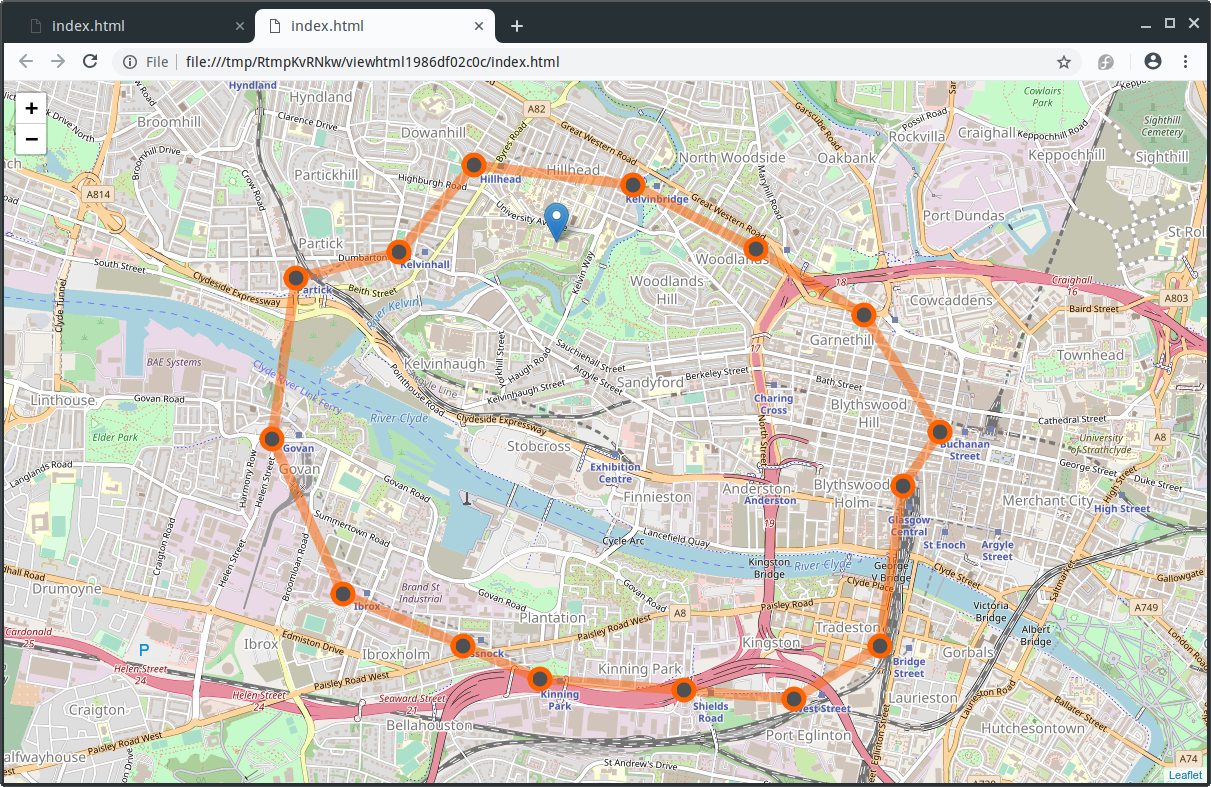
\includegraphics{leaflet2.png}
\caption{Leaflet map showing the Glasgow Subway}
\end{figure}

  \bibliography{book.bib,packages.bib}

\end{document}
